% ******************************************************************************
% A Classic Thesis Style
% An Homage to The Elements of Typographic Style
%
% Copyright (C) 2015 André Miede http://www.miede.de
%
% If you like the style then I would appreciate a postcard. My address
% can be found in the file ClassicThesis.pdf. A collection of the
% postcards I received so far is available online at
% http://postcards.miede.de
%
% License:
% This program is free software; you can redistribute it and/or modify
% it under the terms of the GNU General Public License as published by
% the Free Software Foundation; either version 2 of the License, or
% (at your option) any later version.
%
% This program is distributed in the hope that it will be useful,
% but WITHOUT ANY WARRANTY; without even the implied warranty of
% MERCHANTABILITY or FITNESS FOR A PARTICULAR PURPOSE.  See the
% GNU General Public License for more details.
%
% You should have received a copy of the GNU General Public License
% along with this program; see the file COPYING.  If not, write to
% the Free Software Foundation, Inc., 59 Temple Place - Suite 330,
% Boston, MA 02111-1307, USA.
%
% ******************************************************************************

\RequirePackage{fix-cm} % fix some latex issues see: http://texdoc.net/texmf-dist/doc/latex/base/fixltx2e.pdf

\documentclass[ twoside,openright,titlepage,numbers=noenddot,headinclude,
                footinclude=true,cleardoublepage=empty,abstractoff,
                BCOR=5mm,paper=a4,fontsize=11pt,
                ngerman,american,
                ]{scrreprt}

\usepackage[a-1b]{pdfx}

\usepackage[utf8]{inputenc}
\usepackage{etoolbox}


%% -----------------------------------------------------------------------------

\newcommand{\myTitle}{Collide, Collate, Collect: Recognizing Senders in Wireless Collisions\xspace}
\newcommand{\myDegree}{Bachelor Thesis\xspace}
\newcommand{\myName}{Johannes Tobias Lauinger\xspace}
\newcommand{\myProf}{Prof. Dr.-Ing. Matthias Hollick\xspace}
\newcommand{\mySupervisor}{Robin Klose, M.Sc.\xspace}
\newcommand{\myThesiscode}{SEEMOO-BSC-$0103$\xspace}
\newcommand{\myFaculty}{Department of Computer Science\xspace}
\newcommand{\myDepartment}{Secure Mobile Networking Lab\xspace}
\newcommand{\myUni}{\protect{Technische Universität Darmstadt}\xspace}
\newcommand{\myLocation}{Darmstadt\xspace}
\newcommand{\myTime}{\formatdate{10}{08}{2017}\xspace}
\newcommand{\myVersion}{1.0\xspace}

% Choose if you want the standard template with enough space for margin notes or the tempate with small margins
\newtoggle{adrianstyle}
\toggletrue{adrianstyle}    % uncomment this line to have smaller margins
%\togglefalse{adrianstyle}  % uncomment this line for the standard seemoo template

% ****************************************************************************************************
% classicthesis-config.tex 
% formerly known as loadpackages.sty, classicthesis-ldpkg.sty, and classicthesis-preamble.sty 
% Use it at the beginning of your ClassicThesis.tex, or as a LaTeX Preamble 
% in your ClassicThesis.{tex,lyx} with % ****************************************************************************************************
% classicthesis-config.tex 
% formerly known as loadpackages.sty, classicthesis-ldpkg.sty, and classicthesis-preamble.sty 
% Use it at the beginning of your ClassicThesis.tex, or as a LaTeX Preamble 
% in your ClassicThesis.{tex,lyx} with % ****************************************************************************************************
% classicthesis-config.tex 
% formerly known as loadpackages.sty, classicthesis-ldpkg.sty, and classicthesis-preamble.sty 
% Use it at the beginning of your ClassicThesis.tex, or as a LaTeX Preamble 
% in your ClassicThesis.{tex,lyx} with \input{classicthesis-config}
% ****************************************************************************************************  
% If you like the classicthesis, then I would appreciate a postcard. 
% My address can be found in the file ClassicThesis.pdf. A collection 
% of the postcards I received so far is available online at 
% http://postcards.miede.de
% ****************************************************************************************************

% ****************************************************************************************************
% 1. Configure classicthesis for your needs here, e.g., remove "drafting" below 
% in order to deactivate the time-stamp on the pages
% ****************************************************************************************************
\PassOptionsToPackage{eulerchapternumbers,listings,%
                 %drafting,%
				 pdfspacing,%floatperchapter,%linedheaders,%
				 subfig,beramono,eulermath,parts,dottedtoc,%
				 \iftoggle{adrianstyle}{adrianstyle}{}, % Use this option to increase the text width
				 }{classicthesis}								
% ********************************************************************
% Available options for classicthesis.sty 
% (see ClassicThesis.pdf for more information):
% drafting
% parts nochapters linedheaders
% eulerchapternumbers beramono eulermath pdfspacing minionprospacing
% tocaligned dottedtoc manychapters
% listings floatperchapter subfig
% ********************************************************************


% ****************************************************************************************************
% 2. Loading some handy packages
% ****************************************************************************************************
%\PassOptionsToPackage{spanish,es-lcroman}{babel}

% ********************************************************************
% Setup, finetuning, and useful commands
% ********************************************************************
\newcounter{dummy} % necessary for correct hyperlinks (to index, bib, etc.)
\newlength{\abcd} % for ab..z string length calculation
% ****************************************************************************************************


% ****************************************************************************************************
% 3. Loading some handy packages
% ****************************************************************************************************
% ******************************************************************** 
% Packages with options that might require adjustments
% ******************************************************************** 
%\PassOptionsToPackage{ngerman,american}{babel}   % change this to your language(s)
% Spanish languages need extra options in order to work with this template
%\PassOptionsToPackage{spanish,es-lcroman}{babel}
	\usepackage{babel}                  

\usepackage{csquotes}
\PassOptionsToPackage{%
    %backend=biber, %instead of bibtex
	backend=bibtex8,bibencoding=ascii,%
	language=auto,%
	style=numeric-comp,%
    %style=authoryear-comp, % Author 1999, 2010
    %bibstyle=authoryear,dashed=false, % dashed: substitute rep. author with ---
    sorting=nyt, % name, year, title
    maxbibnames=10, % default: 3, et al.
    %backref=true,%
    natbib=true % natbib compatibility mode (\citep and \citet still work)
}{biblatex}
    \usepackage{biblatex}

\PassOptionsToPackage{fleqn}{amsmath}       % math environments and more by the AMS 
    \usepackage{amsmath}

% ******************************************************************** 
% General useful packages
% ******************************************************************** 
\PassOptionsToPackage{T1}{fontenc} % T2A for cyrillics
    \usepackage{fontenc}     
\usepackage{textcomp} % fix warning with missing font shapes
\usepackage{scrhack} % fix warnings when using KOMA with listings package          
\usepackage{xspace} % to get the spacing after macros right  
\usepackage{mparhack} % get marginpar right
\usepackage{fixltx2e} % fixes some LaTeX stuff --> since 2015 in the LaTeX kernel (see below)
%\usepackage[latest]{latexrelease} % will be used once available in more distributions (ISSUE #107)
\usepackage[nopostdot,acronym,shortcuts,nonumberlist]{glossaries}
\makeglossaries
\renewcommand*{\glossarysection}[2][]{}
\input{acronyms.tex}
% ****************************************************************************************************


% ****************************************************************************************************
% 4. Setup floats: tables, (sub)figures, and captions
% ****************************************************************************************************
\usepackage{tabularx} % better tables
    \setlength{\extrarowheight}{3pt} % increase table row height
\newcommand{\tableheadline}[1]{\multicolumn{1}{c}{\spacedlowsmallcaps{#1}}}
\newcommand{\myfloatalign}{\centering} % to be used with each float for alignment
\usepackage{caption}
% Thanks to cgnieder and Claus Lahiri
% http://tex.stackexchange.com/questions/69349/spacedlowsmallcaps-in-caption-label
% [REMOVED DUE TO OTHER PROBLEMS, SEE ISSUE #82]    
%\DeclareCaptionLabelFormat{smallcaps}{\bothIfFirst{#1}{~}\MakeTextLowercase{\textsc{#2}}}
%\captionsetup{font=small,labelformat=smallcaps} % format=hang,
\captionsetup{font=small} % format=hang,
\usepackage{subfig}  
% ****************************************************************************************************


% ****************************************************************************************************
% 5. Setup code listings
% ****************************************************************************************************
\usepackage{listings} 
%\lstset{emph={trueIndex,root},emphstyle=\color{BlueViolet}}%\underbar} % for special keywords
\lstset{language=[LaTeX]Tex,%C++,
    morekeywords={PassOptionsToPackage,selectlanguage},
    keywordstyle=\color{RoyalBlue},%\bfseries,
    basicstyle=\small\ttfamily,
    %identifierstyle=\color{NavyBlue},
    commentstyle=\color{Green}\ttfamily,
    stringstyle=\rmfamily,
    numbers=none,%left,%
    numberstyle=\scriptsize,%\tiny
    stepnumber=5,
    numbersep=8pt,
    showstringspaces=false,
    breaklines=true,
    %frameround=ftff,
    %frame=single,
    belowcaptionskip=.75\baselineskip
    %frame=L
} 
% ****************************************************************************************************    		   


% ****************************************************************************************************
% 6. PDFLaTeX, hyperreferences and citation backreferences
% ****************************************************************************************************
% ********************************************************************
% Using PDFLaTeX
% ********************************************************************
\PassOptionsToPackage{pdftex,hyperfootnotes=false,pdfpagelabels}{hyperref}
    \usepackage{hyperref}  % backref linktocpage pagebackref
\pdfcompresslevel=9
\pdfadjustspacing=1 
\PassOptionsToPackage{pdftex}{graphicx}
    \usepackage{graphicx} 
 

% ********************************************************************
% Hyperreferences
% ********************************************************************
\hypersetup{%
    %draft,	% = no hyperlinking at all (useful in b/w printouts)
    %colorlinks=true, linktocpage=true, pdfstartpage=3, pdfstartview=FitV,%
    % uncomment the following line if you want to have black links (e.g., for printing)
    colorlinks=false, linktocpage=false, pdfborder={0 0 0}, pdfstartpage=3, pdfstartview=FitV,% 
    breaklinks=true, pdfpagemode=UseNone, pageanchor=true, pdfpagemode=UseOutlines,%
    plainpages=false, bookmarksnumbered, bookmarksopen=true, bookmarksopenlevel=1,%
    hypertexnames=true, pdfhighlight=/O,%nesting=true,%frenchlinks,%
    urlcolor=webbrown, linkcolor=RoyalBlue, citecolor=webgreen, %pagecolor=RoyalBlue,%
    %urlcolor=Black, linkcolor=Black, citecolor=Black, %pagecolor=Black,%
    pdftitle={\myTitle},%
    pdfauthor={\textcopyright\ \myName, \myUni, \myFaculty},%
    pdfsubject={},%
    pdfkeywords={},%
    pdfcreator={pdfLaTeX},%
    pdfproducer={LaTeX with hyperref and classicthesis}%
}

\pdfinfo{
   /CreationDate (D:20130424083342)
   /ModDate (D:20130424083342)
}

% ********************************************************************
% Setup autoreferences
% ********************************************************************
% There are some issues regarding autorefnames
% http://www.ureader.de/msg/136221647.aspx
% http://www.tex.ac.uk/cgi-bin/texfaq2html?label=latexwords
% you have to redefine the makros for the 
% language you use, e.g., american, ngerman
% (as chosen when loading babel/AtBeginDocument)
% ********************************************************************
\makeatletter
\@ifpackageloaded{babel}%
    {%
       \addto\extrasamerican{%
			\renewcommand*{\figureautorefname}{Figure}%
			\renewcommand*{\tableautorefname}{Table}%
			\renewcommand*{\partautorefname}{Part}%
			\renewcommand*{\chapterautorefname}{Chapter}%
			\renewcommand*{\sectionautorefname}{Section}%
			\renewcommand*{\subsectionautorefname}{Section}%
			\renewcommand*{\subsubsectionautorefname}{Section}%     
                }%
       \addto\extrasngerman{% 
			\renewcommand*{\paragraphautorefname}{Absatz}%
			\renewcommand*{\subparagraphautorefname}{Unterabsatz}%
			\renewcommand*{\footnoteautorefname}{Fu\"snote}%
			\renewcommand*{\FancyVerbLineautorefname}{Zeile}%
			\renewcommand*{\theoremautorefname}{Theorem}%
			\renewcommand*{\appendixautorefname}{Anhang}%
			\renewcommand*{\equationautorefname}{Gleichung}%        
			\renewcommand*{\itemautorefname}{Punkt}%
                }%  
            % Fix to getting autorefs for subfigures right (thanks to Belinda Vogt for changing the definition)
            \providecommand{\subfigureautorefname}{\figureautorefname}%             
    }{\relax}
\makeatother


% ****************************************************************************************************
% 7. Last calls before the bar closes
% ****************************************************************************************************
% ********************************************************************
% Development Stuff
% ********************************************************************
\listfiles
%\PassOptionsToPackage{l2tabu,orthodox,abort}{nag}
%   \usepackage{nag}
%\PassOptionsToPackage{warning, all}{onlyamsmath}
%   \usepackage{onlyamsmath}

% ********************************************************************
% Last, but not least...
% ********************************************************************
\usepackage{classicthesis} 
% ****************************************************************************************************


% ****************************************************************************************************
% 8. Further adjustments (experimental)
% ****************************************************************************************************
% ********************************************************************
% Changing the text area
% ********************************************************************
%\linespread{1.05} % a bit more for Palatino
%\areaset[current]{312pt}{761pt} % 686 (factor 2.2) + 33 head + 42 head \the\footskip
%\setlength{\marginparwidth}{7em}%
%\setlength{\marginparsep}{2em}%

% ********************************************************************
% Using different fonts
% ********************************************************************
%\usepackage[oldstylenums]{kpfonts} % oldstyle notextcomp
%\usepackage[osf]{libertine}
%\usepackage[light,condensed,math]{iwona}
%\renewcommand{\sfdefault}{iwona}
%\usepackage{lmodern} % <-- no osf support :-(
%\usepackage{cfr-lm} % 
%\usepackage[urw-garamond]{mathdesign} <-- no osf support :-(
%\usepackage[default,osfigures]{opensans} % scale=0.95 
%\usepackage[sfdefault]{FiraSans}
% ****************************************************************************************************

% ****************************************************************************************************  
% If you like the classicthesis, then I would appreciate a postcard. 
% My address can be found in the file ClassicThesis.pdf. A collection 
% of the postcards I received so far is available online at 
% http://postcards.miede.de
% ****************************************************************************************************

% ****************************************************************************************************
% 1. Configure classicthesis for your needs here, e.g., remove "drafting" below 
% in order to deactivate the time-stamp on the pages
% ****************************************************************************************************
\PassOptionsToPackage{eulerchapternumbers,listings,%
                 %drafting,%
				 pdfspacing,%floatperchapter,%linedheaders,%
				 subfig,beramono,eulermath,parts,dottedtoc,%
				 \iftoggle{adrianstyle}{adrianstyle}{}, % Use this option to increase the text width
				 }{classicthesis}								
% ********************************************************************
% Available options for classicthesis.sty 
% (see ClassicThesis.pdf for more information):
% drafting
% parts nochapters linedheaders
% eulerchapternumbers beramono eulermath pdfspacing minionprospacing
% tocaligned dottedtoc manychapters
% listings floatperchapter subfig
% ********************************************************************


% ****************************************************************************************************
% 2. Loading some handy packages
% ****************************************************************************************************
%\PassOptionsToPackage{spanish,es-lcroman}{babel}

% ********************************************************************
% Setup, finetuning, and useful commands
% ********************************************************************
\newcounter{dummy} % necessary for correct hyperlinks (to index, bib, etc.)
\newlength{\abcd} % for ab..z string length calculation
% ****************************************************************************************************


% ****************************************************************************************************
% 3. Loading some handy packages
% ****************************************************************************************************
% ******************************************************************** 
% Packages with options that might require adjustments
% ******************************************************************** 
%\PassOptionsToPackage{ngerman,american}{babel}   % change this to your language(s)
% Spanish languages need extra options in order to work with this template
%\PassOptionsToPackage{spanish,es-lcroman}{babel}
	\usepackage{babel}                  

\usepackage{csquotes}
\PassOptionsToPackage{%
    %backend=biber, %instead of bibtex
	backend=bibtex8,bibencoding=ascii,%
	language=auto,%
	style=numeric-comp,%
    %style=authoryear-comp, % Author 1999, 2010
    %bibstyle=authoryear,dashed=false, % dashed: substitute rep. author with ---
    sorting=nyt, % name, year, title
    maxbibnames=10, % default: 3, et al.
    %backref=true,%
    natbib=true % natbib compatibility mode (\citep and \citet still work)
}{biblatex}
    \usepackage{biblatex}

\PassOptionsToPackage{fleqn}{amsmath}       % math environments and more by the AMS 
    \usepackage{amsmath}

% ******************************************************************** 
% General useful packages
% ******************************************************************** 
\PassOptionsToPackage{T1}{fontenc} % T2A for cyrillics
    \usepackage{fontenc}     
\usepackage{textcomp} % fix warning with missing font shapes
\usepackage{scrhack} % fix warnings when using KOMA with listings package          
\usepackage{xspace} % to get the spacing after macros right  
\usepackage{mparhack} % get marginpar right
\usepackage{fixltx2e} % fixes some LaTeX stuff --> since 2015 in the LaTeX kernel (see below)
%\usepackage[latest]{latexrelease} % will be used once available in more distributions (ISSUE #107)
\usepackage[nopostdot,acronym,shortcuts,nonumberlist]{glossaries}
\makeglossaries
\renewcommand*{\glossarysection}[2][]{}
\newacronym{MCS}{MCS}{Modulation and Coding Scheme}
\newacronym{OFDM}{OFDM}{Orthogonal Frequency Division Multiplexing}
\newacronym{WARP}{WARP}{Wireless Open-Access Research Platform}
\newacronym{USRP}{USRP}{Universal Software Radio Peripheral}
\newacronym{SDR}{SDR}{Software-Defined Radio}
\newacronym{SDK}{SDK}{Software Development Kit}
\newacronym{SEEMOO}{SEEMOO}{Secure Mobile Networking}
\newacronym{RMS}{RMS}{Root Mean Square}
\newacronym{STF}{STF}{Short Training Field}
\newacronym{LTF}{LTF}{Long Training Field}
\newacronym{AGC}{AGC}{Automatic Gain Control}
\newacronym{FPGA}{FPGA}{Field Programmable Gate Array}
\newacronym{MIMO}{MIMO}{Multiple In Multiple Out}
\newacronym{DCF}{DCF}{Distributed Coordination Function}
\newacronym{RTS}{RTS}{Request To Send}
\newacronym{CTS}{CTS}{Clear To Send}
\newacronym{NAV}{NAV}{Network Allocation Vector}
\newacronym{CSMA/CA}{CSMA/CA}{Carrier Sense Multiple Access with Collision Avoidance}
\newacronym{RSSI}{RSSI}{Received Signal Strength Indicator}
\newacronym{LQI}{LQI}{Link Quality Indicator}
\newacronym{PLFC}{PLFC}{Packet Level Failure Classification}

% ****************************************************************************************************


% ****************************************************************************************************
% 4. Setup floats: tables, (sub)figures, and captions
% ****************************************************************************************************
\usepackage{tabularx} % better tables
    \setlength{\extrarowheight}{3pt} % increase table row height
\newcommand{\tableheadline}[1]{\multicolumn{1}{c}{\spacedlowsmallcaps{#1}}}
\newcommand{\myfloatalign}{\centering} % to be used with each float for alignment
\usepackage{caption}
% Thanks to cgnieder and Claus Lahiri
% http://tex.stackexchange.com/questions/69349/spacedlowsmallcaps-in-caption-label
% [REMOVED DUE TO OTHER PROBLEMS, SEE ISSUE #82]    
%\DeclareCaptionLabelFormat{smallcaps}{\bothIfFirst{#1}{~}\MakeTextLowercase{\textsc{#2}}}
%\captionsetup{font=small,labelformat=smallcaps} % format=hang,
\captionsetup{font=small} % format=hang,
\usepackage{subfig}  
% ****************************************************************************************************


% ****************************************************************************************************
% 5. Setup code listings
% ****************************************************************************************************
\usepackage{listings} 
%\lstset{emph={trueIndex,root},emphstyle=\color{BlueViolet}}%\underbar} % for special keywords
\lstset{language=[LaTeX]Tex,%C++,
    morekeywords={PassOptionsToPackage,selectlanguage},
    keywordstyle=\color{RoyalBlue},%\bfseries,
    basicstyle=\small\ttfamily,
    %identifierstyle=\color{NavyBlue},
    commentstyle=\color{Green}\ttfamily,
    stringstyle=\rmfamily,
    numbers=none,%left,%
    numberstyle=\scriptsize,%\tiny
    stepnumber=5,
    numbersep=8pt,
    showstringspaces=false,
    breaklines=true,
    %frameround=ftff,
    %frame=single,
    belowcaptionskip=.75\baselineskip
    %frame=L
} 
% ****************************************************************************************************    		   


% ****************************************************************************************************
% 6. PDFLaTeX, hyperreferences and citation backreferences
% ****************************************************************************************************
% ********************************************************************
% Using PDFLaTeX
% ********************************************************************
\PassOptionsToPackage{pdftex,hyperfootnotes=false,pdfpagelabels}{hyperref}
    \usepackage{hyperref}  % backref linktocpage pagebackref
\pdfcompresslevel=9
\pdfadjustspacing=1 
\PassOptionsToPackage{pdftex}{graphicx}
    \usepackage{graphicx} 
 

% ********************************************************************
% Hyperreferences
% ********************************************************************
\hypersetup{%
    %draft,	% = no hyperlinking at all (useful in b/w printouts)
    %colorlinks=true, linktocpage=true, pdfstartpage=3, pdfstartview=FitV,%
    % uncomment the following line if you want to have black links (e.g., for printing)
    colorlinks=false, linktocpage=false, pdfborder={0 0 0}, pdfstartpage=3, pdfstartview=FitV,% 
    breaklinks=true, pdfpagemode=UseNone, pageanchor=true, pdfpagemode=UseOutlines,%
    plainpages=false, bookmarksnumbered, bookmarksopen=true, bookmarksopenlevel=1,%
    hypertexnames=true, pdfhighlight=/O,%nesting=true,%frenchlinks,%
    urlcolor=webbrown, linkcolor=RoyalBlue, citecolor=webgreen, %pagecolor=RoyalBlue,%
    %urlcolor=Black, linkcolor=Black, citecolor=Black, %pagecolor=Black,%
    pdftitle={\myTitle},%
    pdfauthor={\textcopyright\ \myName, \myUni, \myFaculty},%
    pdfsubject={},%
    pdfkeywords={},%
    pdfcreator={pdfLaTeX},%
    pdfproducer={LaTeX with hyperref and classicthesis}%
}

\pdfinfo{
   /CreationDate (D:20130424083342)
   /ModDate (D:20130424083342)
}

% ********************************************************************
% Setup autoreferences
% ********************************************************************
% There are some issues regarding autorefnames
% http://www.ureader.de/msg/136221647.aspx
% http://www.tex.ac.uk/cgi-bin/texfaq2html?label=latexwords
% you have to redefine the makros for the 
% language you use, e.g., american, ngerman
% (as chosen when loading babel/AtBeginDocument)
% ********************************************************************
\makeatletter
\@ifpackageloaded{babel}%
    {%
       \addto\extrasamerican{%
			\renewcommand*{\figureautorefname}{Figure}%
			\renewcommand*{\tableautorefname}{Table}%
			\renewcommand*{\partautorefname}{Part}%
			\renewcommand*{\chapterautorefname}{Chapter}%
			\renewcommand*{\sectionautorefname}{Section}%
			\renewcommand*{\subsectionautorefname}{Section}%
			\renewcommand*{\subsubsectionautorefname}{Section}%     
                }%
       \addto\extrasngerman{% 
			\renewcommand*{\paragraphautorefname}{Absatz}%
			\renewcommand*{\subparagraphautorefname}{Unterabsatz}%
			\renewcommand*{\footnoteautorefname}{Fu\"snote}%
			\renewcommand*{\FancyVerbLineautorefname}{Zeile}%
			\renewcommand*{\theoremautorefname}{Theorem}%
			\renewcommand*{\appendixautorefname}{Anhang}%
			\renewcommand*{\equationautorefname}{Gleichung}%        
			\renewcommand*{\itemautorefname}{Punkt}%
                }%  
            % Fix to getting autorefs for subfigures right (thanks to Belinda Vogt for changing the definition)
            \providecommand{\subfigureautorefname}{\figureautorefname}%             
    }{\relax}
\makeatother


% ****************************************************************************************************
% 7. Last calls before the bar closes
% ****************************************************************************************************
% ********************************************************************
% Development Stuff
% ********************************************************************
\listfiles
%\PassOptionsToPackage{l2tabu,orthodox,abort}{nag}
%   \usepackage{nag}
%\PassOptionsToPackage{warning, all}{onlyamsmath}
%   \usepackage{onlyamsmath}

% ********************************************************************
% Last, but not least...
% ********************************************************************
\usepackage{classicthesis} 
% ****************************************************************************************************


% ****************************************************************************************************
% 8. Further adjustments (experimental)
% ****************************************************************************************************
% ********************************************************************
% Changing the text area
% ********************************************************************
%\linespread{1.05} % a bit more for Palatino
%\areaset[current]{312pt}{761pt} % 686 (factor 2.2) + 33 head + 42 head \the\footskip
%\setlength{\marginparwidth}{7em}%
%\setlength{\marginparsep}{2em}%

% ********************************************************************
% Using different fonts
% ********************************************************************
%\usepackage[oldstylenums]{kpfonts} % oldstyle notextcomp
%\usepackage[osf]{libertine}
%\usepackage[light,condensed,math]{iwona}
%\renewcommand{\sfdefault}{iwona}
%\usepackage{lmodern} % <-- no osf support :-(
%\usepackage{cfr-lm} % 
%\usepackage[urw-garamond]{mathdesign} <-- no osf support :-(
%\usepackage[default,osfigures]{opensans} % scale=0.95 
%\usepackage[sfdefault]{FiraSans}
% ****************************************************************************************************

% ****************************************************************************************************  
% If you like the classicthesis, then I would appreciate a postcard. 
% My address can be found in the file ClassicThesis.pdf. A collection 
% of the postcards I received so far is available online at 
% http://postcards.miede.de
% ****************************************************************************************************

% ****************************************************************************************************
% 1. Configure classicthesis for your needs here, e.g., remove "drafting" below 
% in order to deactivate the time-stamp on the pages
% ****************************************************************************************************
\PassOptionsToPackage{eulerchapternumbers,listings,%
                 %drafting,%
				 pdfspacing,%floatperchapter,%linedheaders,%
				 subfig,beramono,eulermath,parts,dottedtoc,%
				 \iftoggle{adrianstyle}{adrianstyle}{}, % Use this option to increase the text width
				 }{classicthesis}								
% ********************************************************************
% Available options for classicthesis.sty 
% (see ClassicThesis.pdf for more information):
% drafting
% parts nochapters linedheaders
% eulerchapternumbers beramono eulermath pdfspacing minionprospacing
% tocaligned dottedtoc manychapters
% listings floatperchapter subfig
% ********************************************************************


% ****************************************************************************************************
% 2. Loading some handy packages
% ****************************************************************************************************
%\PassOptionsToPackage{spanish,es-lcroman}{babel}

% ********************************************************************
% Setup, finetuning, and useful commands
% ********************************************************************
\newcounter{dummy} % necessary for correct hyperlinks (to index, bib, etc.)
\newlength{\abcd} % for ab..z string length calculation
% ****************************************************************************************************


% ****************************************************************************************************
% 3. Loading some handy packages
% ****************************************************************************************************
% ******************************************************************** 
% Packages with options that might require adjustments
% ******************************************************************** 
%\PassOptionsToPackage{ngerman,american}{babel}   % change this to your language(s)
% Spanish languages need extra options in order to work with this template
%\PassOptionsToPackage{spanish,es-lcroman}{babel}
	\usepackage{babel}                  

\usepackage{csquotes}
\PassOptionsToPackage{%
    %backend=biber, %instead of bibtex
	backend=bibtex8,bibencoding=ascii,%
	language=auto,%
	style=numeric-comp,%
    %style=authoryear-comp, % Author 1999, 2010
    %bibstyle=authoryear,dashed=false, % dashed: substitute rep. author with ---
    sorting=nyt, % name, year, title
    maxbibnames=10, % default: 3, et al.
    %backref=true,%
    natbib=true % natbib compatibility mode (\citep and \citet still work)
}{biblatex}
    \usepackage{biblatex}

\PassOptionsToPackage{fleqn}{amsmath}       % math environments and more by the AMS 
    \usepackage{amsmath}

% ******************************************************************** 
% General useful packages
% ******************************************************************** 
\PassOptionsToPackage{T1}{fontenc} % T2A for cyrillics
    \usepackage{fontenc}     
\usepackage{textcomp} % fix warning with missing font shapes
\usepackage{scrhack} % fix warnings when using KOMA with listings package          
\usepackage{xspace} % to get the spacing after macros right  
\usepackage{mparhack} % get marginpar right
\usepackage{fixltx2e} % fixes some LaTeX stuff --> since 2015 in the LaTeX kernel (see below)
%\usepackage[latest]{latexrelease} % will be used once available in more distributions (ISSUE #107)
\usepackage[nopostdot,acronym,shortcuts,nonumberlist]{glossaries}
\makeglossaries
\renewcommand*{\glossarysection}[2][]{}
\newacronym{MCS}{MCS}{Modulation and Coding Scheme}
\newacronym{OFDM}{OFDM}{Orthogonal Frequency Division Multiplexing}
\newacronym{WARP}{WARP}{Wireless Open-Access Research Platform}
\newacronym{USRP}{USRP}{Universal Software Radio Peripheral}
\newacronym{SDR}{SDR}{Software-Defined Radio}
\newacronym{SDK}{SDK}{Software Development Kit}
\newacronym{SEEMOO}{SEEMOO}{Secure Mobile Networking}
\newacronym{RMS}{RMS}{Root Mean Square}
\newacronym{STF}{STF}{Short Training Field}
\newacronym{LTF}{LTF}{Long Training Field}
\newacronym{AGC}{AGC}{Automatic Gain Control}
\newacronym{FPGA}{FPGA}{Field Programmable Gate Array}
\newacronym{MIMO}{MIMO}{Multiple In Multiple Out}
\newacronym{DCF}{DCF}{Distributed Coordination Function}
\newacronym{RTS}{RTS}{Request To Send}
\newacronym{CTS}{CTS}{Clear To Send}
\newacronym{NAV}{NAV}{Network Allocation Vector}
\newacronym{CSMA/CA}{CSMA/CA}{Carrier Sense Multiple Access with Collision Avoidance}
\newacronym{RSSI}{RSSI}{Received Signal Strength Indicator}
\newacronym{LQI}{LQI}{Link Quality Indicator}
\newacronym{PLFC}{PLFC}{Packet Level Failure Classification}

% ****************************************************************************************************


% ****************************************************************************************************
% 4. Setup floats: tables, (sub)figures, and captions
% ****************************************************************************************************
\usepackage{tabularx} % better tables
    \setlength{\extrarowheight}{3pt} % increase table row height
\newcommand{\tableheadline}[1]{\multicolumn{1}{c}{\spacedlowsmallcaps{#1}}}
\newcommand{\myfloatalign}{\centering} % to be used with each float for alignment
\usepackage{caption}
% Thanks to cgnieder and Claus Lahiri
% http://tex.stackexchange.com/questions/69349/spacedlowsmallcaps-in-caption-label
% [REMOVED DUE TO OTHER PROBLEMS, SEE ISSUE #82]    
%\DeclareCaptionLabelFormat{smallcaps}{\bothIfFirst{#1}{~}\MakeTextLowercase{\textsc{#2}}}
%\captionsetup{font=small,labelformat=smallcaps} % format=hang,
\captionsetup{font=small} % format=hang,
\usepackage{subfig}  
% ****************************************************************************************************


% ****************************************************************************************************
% 5. Setup code listings
% ****************************************************************************************************
\usepackage{listings} 
%\lstset{emph={trueIndex,root},emphstyle=\color{BlueViolet}}%\underbar} % for special keywords
\lstset{language=[LaTeX]Tex,%C++,
    morekeywords={PassOptionsToPackage,selectlanguage},
    keywordstyle=\color{RoyalBlue},%\bfseries,
    basicstyle=\small\ttfamily,
    %identifierstyle=\color{NavyBlue},
    commentstyle=\color{Green}\ttfamily,
    stringstyle=\rmfamily,
    numbers=none,%left,%
    numberstyle=\scriptsize,%\tiny
    stepnumber=5,
    numbersep=8pt,
    showstringspaces=false,
    breaklines=true,
    %frameround=ftff,
    %frame=single,
    belowcaptionskip=.75\baselineskip
    %frame=L
} 
% ****************************************************************************************************    		   


% ****************************************************************************************************
% 6. PDFLaTeX, hyperreferences and citation backreferences
% ****************************************************************************************************
% ********************************************************************
% Using PDFLaTeX
% ********************************************************************
\PassOptionsToPackage{pdftex,hyperfootnotes=false,pdfpagelabels}{hyperref}
    \usepackage{hyperref}  % backref linktocpage pagebackref
\pdfcompresslevel=9
\pdfadjustspacing=1 
\PassOptionsToPackage{pdftex}{graphicx}
    \usepackage{graphicx} 
 

% ********************************************************************
% Hyperreferences
% ********************************************************************
\hypersetup{%
    %draft,	% = no hyperlinking at all (useful in b/w printouts)
    %colorlinks=true, linktocpage=true, pdfstartpage=3, pdfstartview=FitV,%
    % uncomment the following line if you want to have black links (e.g., for printing)
    colorlinks=false, linktocpage=false, pdfborder={0 0 0}, pdfstartpage=3, pdfstartview=FitV,% 
    breaklinks=true, pdfpagemode=UseNone, pageanchor=true, pdfpagemode=UseOutlines,%
    plainpages=false, bookmarksnumbered, bookmarksopen=true, bookmarksopenlevel=1,%
    hypertexnames=true, pdfhighlight=/O,%nesting=true,%frenchlinks,%
    urlcolor=webbrown, linkcolor=RoyalBlue, citecolor=webgreen, %pagecolor=RoyalBlue,%
    %urlcolor=Black, linkcolor=Black, citecolor=Black, %pagecolor=Black,%
    pdftitle={\myTitle},%
    pdfauthor={\textcopyright\ \myName, \myUni, \myFaculty},%
    pdfsubject={},%
    pdfkeywords={},%
    pdfcreator={pdfLaTeX},%
    pdfproducer={LaTeX with hyperref and classicthesis}%
}

\pdfinfo{
   /CreationDate (D:20130424083342)
   /ModDate (D:20130424083342)
}

% ********************************************************************
% Setup autoreferences
% ********************************************************************
% There are some issues regarding autorefnames
% http://www.ureader.de/msg/136221647.aspx
% http://www.tex.ac.uk/cgi-bin/texfaq2html?label=latexwords
% you have to redefine the makros for the 
% language you use, e.g., american, ngerman
% (as chosen when loading babel/AtBeginDocument)
% ********************************************************************
\makeatletter
\@ifpackageloaded{babel}%
    {%
       \addto\extrasamerican{%
			\renewcommand*{\figureautorefname}{Figure}%
			\renewcommand*{\tableautorefname}{Table}%
			\renewcommand*{\partautorefname}{Part}%
			\renewcommand*{\chapterautorefname}{Chapter}%
			\renewcommand*{\sectionautorefname}{Section}%
			\renewcommand*{\subsectionautorefname}{Section}%
			\renewcommand*{\subsubsectionautorefname}{Section}%     
                }%
       \addto\extrasngerman{% 
			\renewcommand*{\paragraphautorefname}{Absatz}%
			\renewcommand*{\subparagraphautorefname}{Unterabsatz}%
			\renewcommand*{\footnoteautorefname}{Fu\"snote}%
			\renewcommand*{\FancyVerbLineautorefname}{Zeile}%
			\renewcommand*{\theoremautorefname}{Theorem}%
			\renewcommand*{\appendixautorefname}{Anhang}%
			\renewcommand*{\equationautorefname}{Gleichung}%        
			\renewcommand*{\itemautorefname}{Punkt}%
                }%  
            % Fix to getting autorefs for subfigures right (thanks to Belinda Vogt for changing the definition)
            \providecommand{\subfigureautorefname}{\figureautorefname}%             
    }{\relax}
\makeatother


% ****************************************************************************************************
% 7. Last calls before the bar closes
% ****************************************************************************************************
% ********************************************************************
% Development Stuff
% ********************************************************************
\listfiles
%\PassOptionsToPackage{l2tabu,orthodox,abort}{nag}
%   \usepackage{nag}
%\PassOptionsToPackage{warning, all}{onlyamsmath}
%   \usepackage{onlyamsmath}

% ********************************************************************
% Last, but not least...
% ********************************************************************
\usepackage{classicthesis} 
% ****************************************************************************************************


% ****************************************************************************************************
% 8. Further adjustments (experimental)
% ****************************************************************************************************
% ********************************************************************
% Changing the text area
% ********************************************************************
%\linespread{1.05} % a bit more for Palatino
%\areaset[current]{312pt}{761pt} % 686 (factor 2.2) + 33 head + 42 head \the\footskip
%\setlength{\marginparwidth}{7em}%
%\setlength{\marginparsep}{2em}%

% ********************************************************************
% Using different fonts
% ********************************************************************
%\usepackage[oldstylenums]{kpfonts} % oldstyle notextcomp
%\usepackage[osf]{libertine}
%\usepackage[light,condensed,math]{iwona}
%\renewcommand{\sfdefault}{iwona}
%\usepackage{lmodern} % <-- no osf support :-(
%\usepackage{cfr-lm} % 
%\usepackage[urw-garamond]{mathdesign} <-- no osf support :-(
%\usepackage[default,osfigures]{opensans} % scale=0.95 
%\usepackage[sfdefault]{FiraSans}
% ****************************************************************************************************

\usepackage{tikz}
\usetikzlibrary{dsp,chains}
\usepackage{pgfplots}
%\pgfplotsset{compat=newest}
\usetikzlibrary{positioning}
\DeclareMathAlphabet{\mathpzc}{OT1}{pzc}{m}{it}
\newcommand{\z}{\mathpzc{z}}
\usepackage{float}
\usepackage{scalefnt}

\usepackage{lipsum}

% To cache tikz pictures you have to run pdflatex with -shell-escape or --enable-write18
\ifnum\pdfshellescape=1
\usepgfplotslibrary{external}
\tikzexternalize[prefix=gfxcompiled/]
%\tikzset{external/remake next}
%\tikzset{external/force remake}
\newcommand{\tikzremakenext}{\tikzset{external/remake next}}
%\tikzexternalize[shell escape=-enable-write18]
\else
\newcommand{\tikzremakenext}{}
\fi

%lengths for matlab2tikz
\newlength\figureheight
\newlength\figurewidth


\usepackage{textpos}
\usepackage{datetime}
\usepackage{changepage}

% move lstlisting captions to the left
%\usepackage{caption}
%\captionsetup[lstlisting]{singlelinecheck=off}

% setup Matlab syntax highlighting
\lstset{language=Matlab,%
    breaklines=true,%
    morekeywords={matlab2tikz},
    keywordstyle=\color{blue},%
    morekeywords=[2]{1}, keywordstyle=[2]{\color{black}},
    identifierstyle=\color{black},%
    stringstyle=\color{lilas},
    commentstyle=\color{green!60!black},%
    showstringspaces=false,%without this there will be a symbol in the places where there is a space
    numbers=left,%
    numberstyle={\tiny \color{black}},% size of the numbers
    numbersep=9pt, % this defines how far the numbers are from the text
    emph=[1]{for,end,break},emphstyle=[1]\color{red}, %some words to emphasise
    %emph=[2]{word1,word2}, emphstyle=[2]{style},
}

\hyphenation{
	Si-mu-link
	OO-WARP-Lab
	WARP-Lab
}

\addbibresource{config/bibliography.bib}


%% -----------------------------------------------------------------------------

\begin{document}

\frenchspacing
\raggedbottom
\selectlanguage{american}
\pagenumbering{roman}
\pagestyle{plain}
\setlength\parindent{0pt}


%% -----------------------------------------------------------------------------

%*******************************************************
% Titlepage
%*******************************************************
\begin{titlepage}

    %\begin{comment}
    %\begin{textblock*}{297mm}(0mm,0mm)
    %    \includegraphics[width=\paperwidth]{gfx/titlePage}
    %\end{textblock*}
    %\phantom{Invisible, but important}
    %\newpage
    %\end{comment}

	% if you want the titlepage to be centered, uncomment and fine-tune the line below (KOMA classes environment)
	\begin{addmargin}[-0.5cm]{\iftoggle{adrianstyle}{-2cm}{-3.5cm}}
    \begin{center}
        \large

        
\includegraphics[width=6cm]{gfx/logos/tud_logo}
        
        \vfill

        \begingroup
            %\color{Maroon}\spacedallcaps{\myTitle} \\ \bigskip
            \color{Maroon}\spacedallcaps{\myTitle} \bigskip
        \endgroup

        \spacedlowsmallcaps{\myName}

        \vfill

        \medskip

        \myDegree \\ \medskip
        \myTime

        \bigskip

        \vfill

        \myDepartment \\
        \myFaculty \\[0.2cm]
        %\myUni \\
        
\includegraphics[width=5cm]{gfx/logos/seemoo_logo} \\

        %\vfill

    \end{center}
    \end{addmargin}
\end{titlepage}   
\thispagestyle{empty}
\begin{adjustwidth}{\iftoggle{adrianstyle}{-1.75cm}{-4cm}}{}
\noindent\myTitle \\
\noindent\myDegree \\
\noindent\myThesiscode

\bigskip

\noindent Submitted by \myName \\
\noindent Date of submission: \myTime

\bigskip

\noindent Advisor: \myProf

\noindent Supervisor: \mySupervisor


\hfill

\vfill

\noindent \myUni \\
\noindent \myFaculty \\
\noindent \myDepartment \\
\end{adjustwidth}
\cleardoublepage%% -----------------------------------------------------------------------------
% Abstract

%% -----------------------------------------------------------------------------
% English version

\pdfbookmark[1]{Abstract}{Abstract}
\begingroup
\let\clearpage\relax
\let\cleardoublepage\relax
\let\cleardoublepage\relax

\chapter*{Abstract}

With wireless mobile IEEE 802.11a/g networks, collisions are currently inevitable despite effective counter measures. This work proposes an approach to detect the MAC addresses of transmitting stations in case of a collision, and measures its practical feasibility. Recognizing senders using cross-correlation in the time domain worked surprisingly well in simulations using Additive White Gaussian Noise (AWGN) and standard Matlab channel models.\\

Real-world experiments using software-defined radios also showed promising results in spite of decreased accuracy due to channel effects. During the experiments, various Modulation and Coding Schemes (MCSs) and scrambler initialization values were compared. Knowledge about which senders were transmitting leading up to a collision could help develop new improvements to the 802.11 MAC coordination function, or serve as a feature for learning-based algorithms.


%% -----------------------------------------------------------------------------
% German version

\vfill
\selectlanguage{ngerman}
\pdfbookmark[1]{Zusammenfassung}{Zusammenfassung}
\chapter*{Zusammenfassung}

In drahtlosen mobilen Netzwerken nach den IEEE 802.11a/g Standards sind Kollisionen trotz wirkungsvoller Gegenmaßnahmen nicht vollständig zu vermeiden. Diese Arbeit stellt einen Ansatz zur Erkennung der MAC-Adressen der beteiligten Sender bei einer Kollision vor und untersucht, inwiefern das Verfahren in der Praxis funktioniert. Über Kreuzkorrelation im Zeitbereich funktionierte die Erkennung in Simulationen unter Additivem Weißen Gaußschen Rauschen (AWGN) und verschiedenen Standard-Kanalmodellen von Matlab erstaunlich gut.\\

Praktische Experimente mit Software-Defined Radios zeigten ebenfalls vielversprechende Ergebnisse, wenn auch die Genauigkeit der Erkennung durch Kanaleffekte beeinträchtigt wurde. Bei den Experimenten wurden verschiedene Modulation and Coding Schemes (MCSs) und Scrambler-Initialisierungen verglichen. Die Kenntnis über die beteiligten Sender bei einer Kollision könnte zur Verbesserung der Koordinierungsfunktion oder als Feature für lernbasierte Verfahren verwendet werden.


\selectlanguage{american}
\endgroup
\vfill


\pagestyle{scrheadings}
\cleardoublepage%% ---------------------------------------------------------------------------------------------------------------------
% Table of Contents


%\phantomsection
\refstepcounter{dummy}
\pdfbookmark[1]{\contentsname}{tableofcontents}
\setcounter{tocdepth}{2} % <-- 2 includes up to subsections in the ToC
\setcounter{secnumdepth}{3} % <-- 3 numbers up to subsubsections
\manualmark
\markboth{\spacedlowsmallcaps{\contentsname}}{\spacedlowsmallcaps{\contentsname}}
%\begin{adjustwidth}[]{}{-4cm}
\tableofcontents 
%\end{adjustwidth}
\automark[section]{chapter}
\renewcommand{\chaptermark}[1]{\markboth{\spacedlowsmallcaps{#1}}{\spacedlowsmallcaps{#1}}}
\renewcommand{\sectionmark}[1]{\markright{\thesection\enspace\spacedlowsmallcaps{#1}}}


%% ---------------------------------------------------------------------------------------------------------------------
% List of Figures and of the Tables

\clearpage

\begingroup 
    \let\clearpage\relax
    \let\cleardoublepage\relax
    \let\cleardoublepage\relax
    
    %*******************************************************
    % List of Figures
    %*******************************************************    
    %\phantomsection 
    \refstepcounter{dummy}
    %\addcontentsline{toc}{chapter}{\listfigurename}
    \pdfbookmark[1]{\listfigurename}{lof}
    \enlargethispage{6em}
    \listoffigures
    \enlargethispage{6em}

%	\newpage

    \vspace{8ex}
    

    %*******************************************************
    % List of Tables
    %*******************************************************
    %\phantomsection 
    \refstepcounter{dummy}
    %\addcontentsline{toc}{chapter}{\listtablename}
    \pdfbookmark[1]{\listtablename}{lot}
    \listoftables
        
    \vspace*{8ex}
%   \newpage
    
    %*******************************************************
    % List of Listings
    %*******************************************************      
	  %\phantomsection 
    \refstepcounter{dummy}
    %\addcontentsline{toc}{chapter}{\lstlistlistingname}
    \pdfbookmark[1]{\lstlistlistingname}{lol}
    \lstlistoflistings 

    \vspace*{8ex}
    \newpage
       
    %*******************************************************
    % Acronyms
    %*******************************************************
    %\phantomsection 
    \refstepcounter{dummy}
    \pdfbookmark[1]{Acronyms}{acronyms}
    \markboth{\spacedlowsmallcaps{Acronyms}}{\spacedlowsmallcaps{Acronyms}}
    \chapter*{Acronyms}
    %\glsaddall
    \printglossary[type=\acronymtype,style=long]

\endgroup

\cleardoublepage

\pagenumbering{arabic}
\setcounter{table}{0}


%% -----------------------------------------------------------------------------

%% ---------------------------------------------------------------------------------------------------------------------
\chapter{Introduction}\label{ch:introduction}

\glsresetall % Resets all acronyms to not used


%% ---------------------------------------------------------------------------------------------------------------------

Start a chapter with text and not with a section header. Open the
\emph{classicthesis-config.tex} file to insert the title of your thesis, the
names of your supervisors and the hand-in date of your thesis.


%% ---------------------------------------------------------------------------------------------------------------------

\section{First Section}
\label{sec:first_section}

After a section there should always be text before the next section. The first
paragraph is always without indentation. Starting from the second paragraph,
there is an indentation.

Here is an equation that you can reference:
\begin{align}
\underbrace{\begin{pmatrix}\mathcal{B}_1\\\mathcal{B}_2\\\vdots\\\mathcal{B}_R\end{pmatrix}}_\mathcal{B} &= \underbrace{\begin{pmatrix}H_{1,1} & H_{1,2} & \hdots & H_{1,T}\\H_{2,1} & H_{2,2} & \hdots & H_{2,T}\\\vdots & \vdots & \ddots & \vdots\\H_{R,1} & H_{R,2} & \hdots & H_{R,T}\end{pmatrix}}_{H_{A\rightarrow B}}\cdot \underbrace{\begin{pmatrix}\mathcal{A}_1\\\mathcal{A}_2\\\vdots\\\mathcal{A}_T\end{pmatrix}}_\mathcal{A}\label{eqn:example}
\end{align}


\subsection{Referencing}

Take a look in the following list to reference sections, figures and equations:
\begin{itemize}
  \item \autoref{sec:first_section}
  \item \autoref{fig:wiretapchannel}
  \item \autoref{eqn:example}
\end{itemize}


\subsection{Acronyms}
For acronyms you should use the \emph{glossaries} package and put your acronyms
in the \emph{FrontBackmatter/acronyms.tex} file. The first acronym is always
written in it's long form, the following occurrences are abbreviated: first
occurrence \gls{SNR}, second occurrence \gls{SNR}, plural \glspl{SNR}.


\subsection{Examples on Figures}

\sloppy
When using figures, use vector graphics whenever possible. In
\autoref{fig:wiretapchannel} and \autoref{fig:example} are some examples to
generate vector graphics directly from \LaTeX code. The second example is based
on the \emph{matlab2tikz} script for matlab. You find an example in the
\mbox{\emph{gfx/matlab/create\_example\_graph.m}} file. TikZ is used to generate
the graphics. As it takes some time and memory to recompile a graphic, pdflatex
caches generated figures when the \lstinline|--enable-write18| switch is set
when calling \lstinline|pdflatex|. Graphics are only recompiled when you
uncomment the \lstinline|\tikzset{external/remake next}| command. Figures should
always appear after the first reference in the text or at the top of the same
page as the reference, but never before the reference. Prefer placing figures on
separate pages. Try to always have figures and text on each page. Or place
enough figures to fill a page only with figures.

\begin{figure}
\centering
\begin{tikzpicture}[node distance=6mm]
\node[dspsquare,minimum height=3.2em, minimum width=5em,text height=1em, fill=white]
		(source) {Source};
\node[dspsquare,minimum height=3.2em, minimum width=5em,text height=1em, fill=white, right=of source]
		(encoder) {Encoder};
\node[dspsquare,minimum height=3.2em, minimum width=7em,text height=2em, fill=white, right=of encoder]
		(mainch) {Main Channel\\$Q_M$};
\node[dspnodefull, right=of mainch] (n1) {};
\node[dspsquare,minimum height=3.2em, minimum width=5em,text height=1em, fill=white, right=of n1]
		(decoder) {Decoder};
\node[coordinate,right=of decoder] (n2) {};
\node[dspsquare,minimum height=3.2em, minimum width=10em,text height=2em, fill=white, below=1cm of n1]
		(wiretapch) {Wiretap Channel\\$Q_W$};
\node[coordinate,below=of wiretapch] (n3) {};

\draw[dspconn] (source) -- node[midway,above] {$S^K$} (encoder);
\draw[dspconn] (encoder) -- node[midway,above] {$X^N$} (mainch);
\draw[dspconn] (mainch) -- node[midway,above] {$Y^N$} (decoder);
\draw[dspconn] (decoder) -- node[midway,above] {$S^K$} (n2);
\draw[dspconn] (n1) -- (wiretapch);
\draw[dspconn] (wiretapch) -- (n3) node[below] {$Z^N$};
\end{tikzpicture}
\caption[The wiretap channel]{The wiretap channel (source: \cite{1975:Wyner})}
\label{fig:wiretapchannel}
\end{figure}


%% ---------------------------------------------------------------------------------------------------------------------

\section{Margin Notes}

Especially in the standard SEEMOO template with wide margins, you are
\marginpar{Here you can add text to the margin. For example, to
summarize the section next to it.} encouraged to insert text into the
margins. If you decide to do so, plan to have at least one margin note
per double page.

%% -----------------------------------------------------------------------------

\chapter{Background}\label{ch:relatedwork}
\glsresetall % Resets all acronyms to not used

This chapter provides an introduction to the overall structure of the IEEE 802.11 standards for wireless networks. It covers the parts that are essential to recognizing sender MAC addresses. Furthermore, background information on cross-correlation is given.


%% -----------------------------------------------------------------------------

\section{IEEE 802.11 MAC and PHY} \label{sec:mac-and-phy}

The IEEE 802.11 standards family describes wireless local area networks as supported by all current major operating platforms. IEEE 802.11 networks inherit the reference structure of their parent standard, IEEE 802. Specifically, they share the 6 byte device addresses used to identify a physical network interface, which is called MAC address.

The standard is devided in the physical (PHY), and the medium access control (MAC) layer specifications. Logical link control (LLC) as described by the IEEE 802.2 standard is shared with euqivalent wired networks.


\subsection{Physical Layer Specification}

There are a number of different physical layer specifications available for use in IEEE 802.11 networks, which define various parameters such as the frequency used for transmissions.

In this work, I restrain usage to the IEEE 802.11 a/g standards. These use orthogonal frequency division multiplexing (ODFM) to distribute bits over a channel spectrum. The maximum achievable data rate is 54 megabits per second (Mbps) \cite{ieee2012}. The most significant difference between the two is that 802.11a uses a carrier frequency of 5 GHz, whereas 802.11g transmits on 2.4 GHz. Around the carrier frequency, multiple channels of 20 MHz bandwidth are available. These PHY standards are extremely widely supported but were superseded by the 802.11n specification some time ago.

With 802.11n, being the first high-throughput standard, channels with more bandwidth and multiple spatial streams (MIMO) were introduced, providing a much higher data rate. 802.11ac and the currently in-development 802.11ax improve even further on that. However, due to their higher complexity, I leave adaption of my sender detection evaluation for future work.\\

The physical layer frame structure comprises several data fields. They are illustrated in figure \ref{fig:phy-format}. The physical service data unit (PSDU) is the payload which is passed down for transmission by the MAC layer. It is encapsulated within the 16 bits service field (SRV) in the beginning, and 6 tail bits and padding in the end. The combination of these is called data field (DATA).

The data field is modulated with the following process: First, the bits are scrambled by applying XOR with a synchronous bit sequence. This scrambling sequence is repeatedly generated by a linear feedback shift register derived by the polynomial $G(D)=D^7+D^4+1$, having a 7 bit state register. When transmitting, the initial scrambler state should be set to a pseudo-random non-zero state for each packet \cite{ieee2012}. Since the service field, as described earlier, is prepended with all bits set to zero, the first seven bits contain the initialization value after scrambling. This is because for any value A, it holds $A \oplus 0 = A$. When receiving a frame in normal operation, the service field is used to synchronize the descrambler to that same initialization.

\begin{figure}[H]
	\centering
	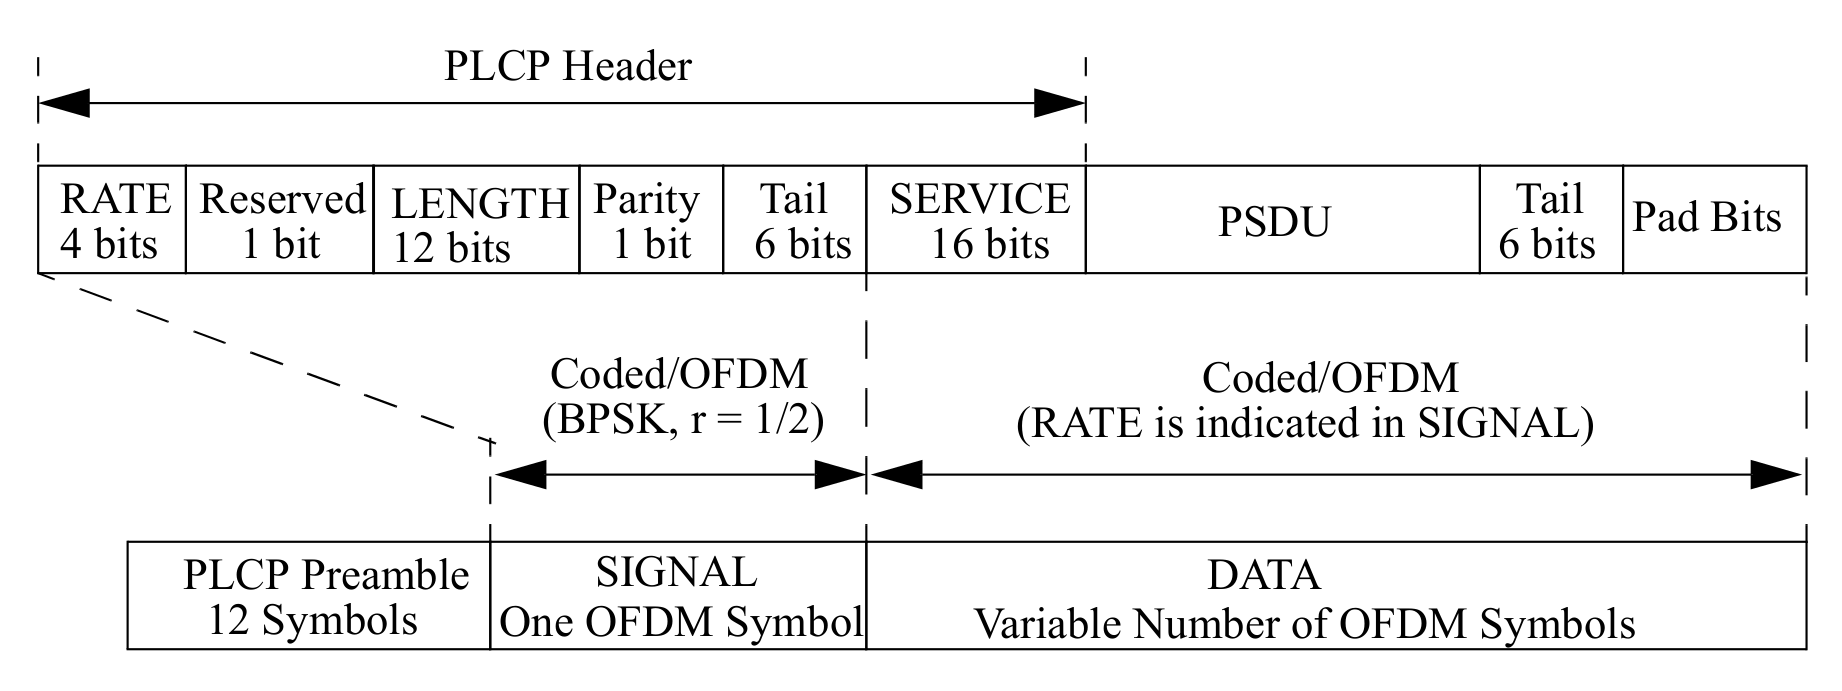
\includegraphics[width=\textwidth]{gfx/images/phy-format}
	\caption[IEEE 802.11 Physical Layer Frame Structure]{IEEE 802.11 Physical Layer Frame Structure \cite{ieee2012}}
	\label{fig:phy-format}
\end{figure}

After that, convolutional encoding is applied to the bits. The standard allows the encoder to use different code rates as specified by the modulation and coding schemes (MCS). The encoder also uses a 7 bit state \cite{park2009}. Next, bits are grouped into symbols and rearranged using a deterministic permutation function \cite{perahia2013}. This is called interleaving. Following this, the symbols are modulated using quadrature amplitude modulation (QAM)	with different possible bit rates.\\

The available constellations are described by the modulation and coding scheme. Table \ref{tbl:mcs} shows all available MCS for IEEE 802.11 a/g. Finally, pilot signals are added, the signal is transformed into the time-domain using the inverse fast fourier transform, a cyclic prefix is added, and the signal is further processed and sent.

\begin{table}[ht]
	\centering
	\begin{tabular}{|p{2.5cm}|p{2.5cm}|p{2.5cm}|p{2.5cm}|p{2.5cm}|}
		\hline
		\textbf{MCS} & \textbf{Modulation} & \textbf{Coding Rate} & \textbf{Coded bits per symbol} & \textbf{Data bits per symbol} \\ \hline
		0 & BPSK & 1/2 & 48 & 24 \\ \hline
		1 & BPSK & 3/4 & 48 & 36 \\ \hline
		2 & QPSK & 1/2 & 96 & 48 \\ \hline
		3 & QPSK & 3/4 & 96 & 72 \\ \hline
		4 & 16QAM & 1/2 & 192 & 96 \\ \hline
		5 & 16QAM & 3/4 & 192 & 144 \\ \hline
		6 & 64QAM & 2/3 & 288 & 192 \\ \hline
		7 & 64QAM & 3/4 & 288 & 216 \\ \hline
	\end{tabular}
	\caption[IEEE 802.11 a/g Modulation and Coding Schemes]{IEEE 802.11 a/g Modulation and Coding Schemes (MCS) \cite{ieee2012} \label{tbl:mcs}}
\end{table}

The signal field (SIG), which is transmitted before the data field, contains the MCS used for the frame, and its length in octets. The signal field is always modulated with binary phase shift keying (BPSK) and rate $\frac{1}{2}$ binary convolution code (BCC). Nearby stations will also decode the SIG to defer their transmissions for an appropriate time. The signal field has a duration of 4 $\mu$s.\\

In order to allow the receiver to calculate path effects of the channel, and to equalize received data, training fields are used in the beginning of the frame. The Short Training Field (STF) is used for start-of-frame detection and automatic gain control (AGC). It includes 10 repetitions of a 0.8 $\mu$s symbol, resulting in a duration of 8 $\mu$s. The sequence is chosen to have good correlation properties and a low peak-to-average power, meaning its properties are preserved after clipping \cite{perahia2013}.

The Long Training Field (LTF) is used for channel estimation, more precise frequency offset estimation, and time synchronization. It comprises 2 repetitions of a 3.2 $\mu$s training symbol, and 1.6 $\mu$s cyclic prefix, therefore the LTF also spans 8 $\mu$s. Both training fields and the signal field form the preamble. Figure \ref{fig:preamble} shows detailed timing information for that.

\begin{figure}[H]
	\centering
	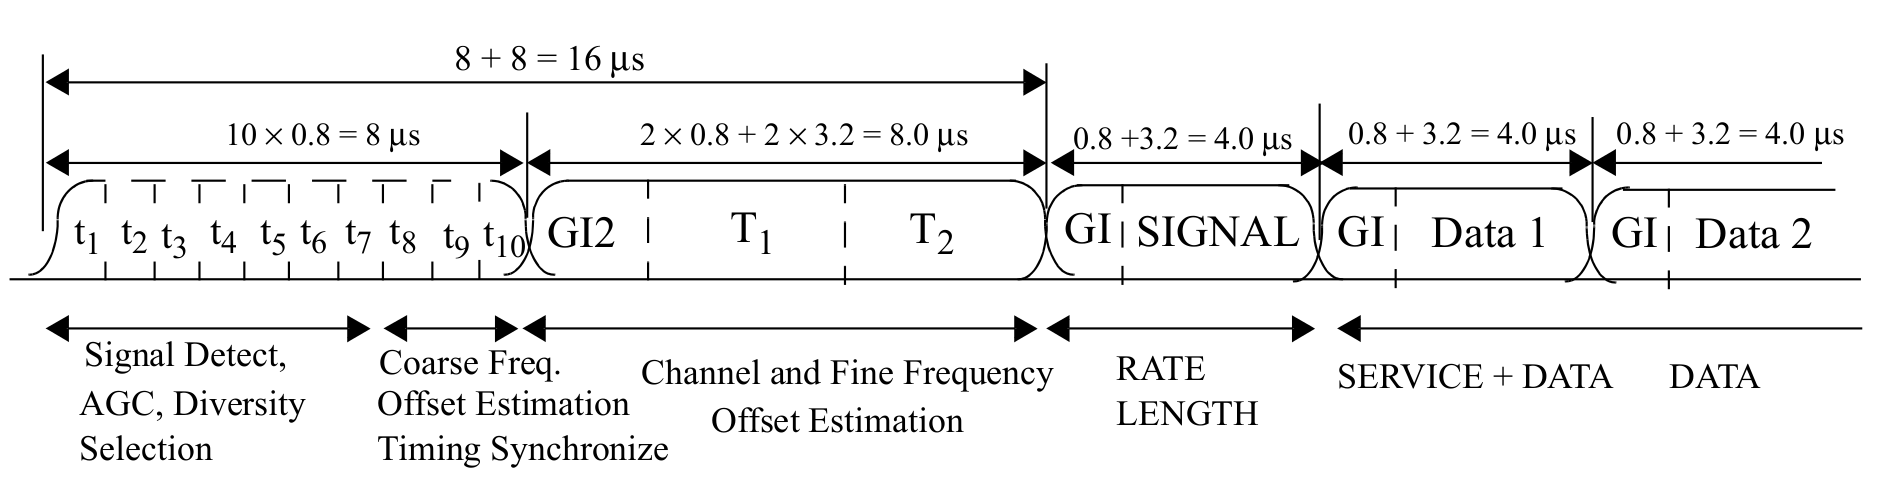
\includegraphics[width=\textwidth]{gfx/images/preamble-format}
	\caption[IEEE 802.11 Preamble Timing]{IEEE 802.11 Preamble Timing \cite{ieee2012}}
	\label{fig:preamble}
\end{figure}


\subsection{Medium Access Control Layer Specification} \label{sec:mac-format}

The medium access control layer (MAC) controls which station may transmit at a given time. The IEEE 802.11 MAC layer uses carrier sense multiple access with collision avoidance (CSMA/CA). With this algorithm, every station listens to the medium before a transmission. Collisions are prevented if possible, and detected through the lack of an acknowledgement packet. In contrast, Ethernet uses CSMA/CD (collision detection), where a transmitting station can directly sense a collision \cite{ieee802-3}.\\

A MAC frame includes a MAC header, a variable-length body, and a frame check sequence (FCS) containing a cyclic redundancy check code (CRC).

The MAC header consists of 2 byte frame control, 2 byte frame duration in microseconds, 18 bytes address 1, 2 and 3, as well some others depending on the frame control field. In a data frame, the address fields contain the receive address (RA), transmit address (TA), and the BSSID. The frame structure is illustrated in figure \ref{fig:mac-format}.

\begin{figure}[H]
	\centering
	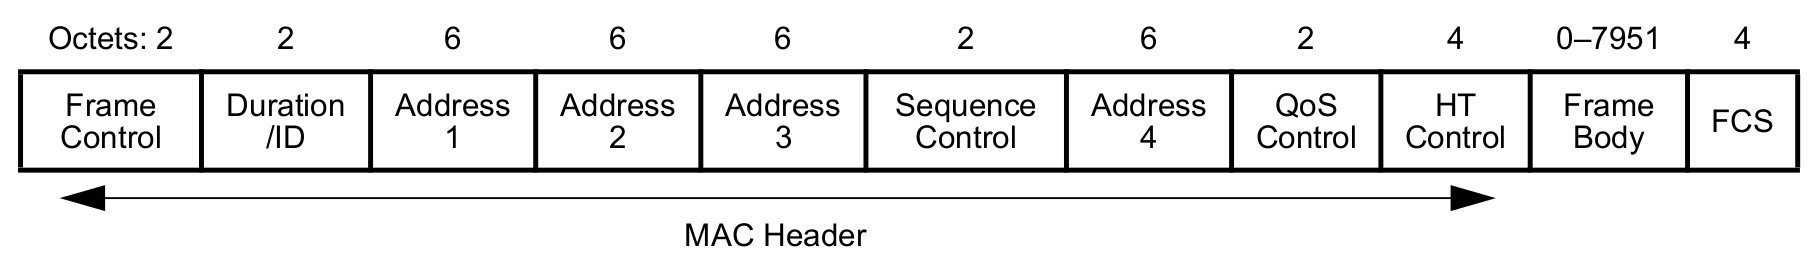
\includegraphics[width=\textwidth]{gfx/images/mac-format}
	\caption[IEEE 802.11 MAC Layer Frame Structure]{IEEE 802.11 MAC Layer Frame Structure \cite{ieee2012}}
	\label{fig:mac-format}
\end{figure}


%% -----------------------------------------------------------------------------

\section{Distributed Coordination Function}\label{sec:dcf}

The Distributed Coordination Function (DCF) describes precisely when sending stations may transmit. It logically belongs to the MAC layer. A station may send after sensing the medium idle for at least one DIFS (DCF inter-frame space) \cite{bianchi2000}. While a sender has access to the medium, it separates frames by a SIFS (short inter-frame space), and other stations will not capture the medium because they must wait for a longer DIFS.

After sensing the medium idle for a DIFS, a station must wait a random backoff time before transmitting. This helps reduce collisions caused by multiple stations waiting to transmit. The backoff time is pseudo-randomly chosen out of the interval $[0..CW]$, where CW is the so-called contention window. On each unsuccessful transmit, CW is doubled. It is reset to its initial value as specified by the standard after a successful transmission.\\

The IEEE 802.11 MAC uses positive frame acknowledgements by layer 2 ACK frames. Without an ACK the sender retransmits the frame. To further reduce collision impact, large payloads are fragmented into multiple PSDUs, which are acknowledged individually. Data frames include a retry bit in the sequence number field to detect duplicate frames \cite{perahia2013}.\\

The hidden node problem can occur when a station sees the access point (AP), but not a third station that is currently transmitting to the AP. The medium is busy, but the first station senses it as idle and begins a transmission. Therefore, the transmission to the AP is subject to a collision. One approach to mitigate this is using an additional handshake mechanism before transmitting:

Before sending the data packet, a station transmits a request to send frame (RTS) containing the desired sending duration. The access point will reply with a clear to send frame (CTS), and third stations update a network allocation vector (NAV) to remember the busy medium. In the hidden node scenario, the offending station would be able to receive the CTS frame from the AP, therefore knowing of the ongoing transmission. On top of that, RTS frames are much shorter than data frames, meaning a collision is less harmful to the medium because less airtime is wasted.


%% -----------------------------------------------------------------------------

\section{Cross-Correlation}

The cross-correlation is a function of two continuous or discrete series that measures their similarity \cite{rabiner1978}. It is often used to compare different functions, or to search for a small feature in a larger stream of data.

With IEEE 802.11, cross-correlation is applied to find the beginning of packets by correlating a known symbol of the short or long training field with a sample stream as captured by a receiver. However, in this thesis I will use it to also correlate the time-domain representation of MAC addresses.\\

Since wireless transmission samples are discrete values, I disregard the continuous form of cross-correlation here. The discrete variant for series of samples f and g is calculated as follows:

$$ (f \star g)(n) = \sum_{m=-\infty}^{\infty} f^{\ast}(m) g(m+n) $$\vspace{0cm}

This formula is related to the convolution of the values, but it features the complex conjugate of the first function for the sum of products. A graphic analogy for cross-correlation would be sliding the functions against each other, where for each point all function values are multiplied individually and then added up.

In general, higher values of cross-correlations mean that the functions are more similar. It is worth noting that periodic functions have periodic cross-correlations, and that the IEEE 802.11 Long Training Field is designed specifically in such a way that correlation is many orders of magnitude higher if the samples of two copies overlap exactly, than it is for any other alignment \cite{perahia2013}.


%% -----------------------------------------------------------------------------

\section{Multi-Path Channel Effects}\label{sec:multipath}

In an ideal scenario, a transmitted signal would travel on a direct line of sight from sender to receiver. However, electromagnetic waves spread in a spherical shape. In a real-world situation, signals can therefore reach the receiver on multiple paths, each affected by different delay, attenuation, reflection, or other effects.

A common multi-path effect are echoes, which are caused by signals being reflected on walls, furniture, or similar obstacles. When an echo occurs, an attenuated copy of the signal with a delay is received.\\

When trying to decode collisions, or detect affected senders, it is therefore important to take multi-path interference into account. Especially devastating is the fact that the signals add up at the receiving antenna. This means that the training fields in the preamble are affected by different paths and can hardly be used to calculate the inverted channel matrix. Chapter 5 provides more details on this problem.

%% -----------------------------------------------------------------------------

\chapter{Related Work}\label{ch:relatedwork}
\glsresetall % Resets all acronyms to not used
\glsunset{IEEE} \glsunset{MAC}

In this chapter I present related research and relevant previous work. The later proposed technique of recognizing senders in a collision by correlating their \gls{MAC} addresses in the time domain has to my best knowledge not been described in the literature yet. However, there have been experiments which point towards that idea. This chapter is organized in sections dealing with the coordination function, hidden terminals, collision handling, and consequences of the capture effect.


%% -----------------------------------------------------------------------------

\section{Improvements To and Alternative DCFs}\label{sec:related-dcf}

As described in section \ref{sec:dcf}, the \gls{DCF} defines the rules of communication in an IEEE 802.11 network. There are measures to reduce the impact of a collision, such as the two-way handshake using \gls{RTS} and \gls{CTS} frames. This procedure allows stations in the network to request transmission for a specific time. Other stations can listen to this \gls{RTS} and update their \gls{NAV} tables accordingly. If a collision occurs, it will happen on the \gls{RTS} frame. Since the \gls{RTS} frame is much shorter than a data frame, the amount of unusable air-time is smaller, as less data has to be discarded.

Giuseppe Bianchi contributed a performance analysis of the \gls{DCF} \cite{bianchi2000}. The maximum load that the system can carry in stable condition is called saturation throughput. The author develops a Markov model to derive throughput estimations and verifies them against simulations. A result is that using the two-way handshake is not effective in practice. The throughput did not increase in experiments which are comparable to a  typical wireless application, mostly due to the overhead introduced by the additional \gls{RTS} and \gls{CTS} frames. Therefore, \gls{RTS} and \gls{CTS} frames are not used in most network configurations nowadays \cite{bianchi2000, gollakota2008, choi2013}.\\

ReCoder \cite{meng2015} is an algorithm for neighbor discovery in 802.11 networks that does not use beacon frames. Instead, a new frame format that only needs to be correlated, not decoded, is introduced. The technique saves energy and is more resilient to collisions, since the otherwise necessary decoding of the frame is not possible in that situation.

These alternative frames start with a fixed, independent training sequence called RCover. This sequence is used to identify a neighbor discovery message, similar to frame detection using the Short Training Field. After that, a two-stage identification pattern is applied. The first stage is a fixed Gold-code signal with low off-peak autocorrelation, shifted by a unique amount of samples. These are chosen randomly by the sending station. In the event that two stations choose the same offset, they are distinguished by the second stage, which is a hash of the \gls{MAC} address. This stage is less distinguishable and therefore only acts as a tie-beaker for identical first stages.\\

Receivers are triggered by the RCover sequence and correlate the first identity stage to the list of known stations. If a match is found, the second stage is checked to eliminate possible duplicate shift-amounts. If however no match is found, the reference table is adjusted in a way that the new identity is now included.\\

As Zhu et al. pointed out, real-world packet loss can be caused by both a weak link, and collisions. These conditions can change very fast \cite{zhu2015}. Reasons for this include humans being in the signal path, external interference, and unpredictable transmissions by other stations. Distinguishing failure conditions must thus be done at the frame level to provide useful information. Both naive assumptions of only collisions, or only weak links, cause a waste of resources, i.e. air-time or transmission power.

The authors present a new algorithm, \gls{PLFC}, which collects a byte-level \gls{RSSI} and a packet-level \gls{LQI}. Using this information, the receiver provides the sender with an elaborated retransmission request. This includes whether there was a weak link or a collision. The sender can then for example increase transmission power to mitigate a weak link, or just retransmit if a collision occurred \cite{zhu2015}.\\

For continuous and fairly regular data streams from multiple clients, such as in an environment with several VoIP transmissions, the 802.11 \gls{MAC} exponential backoff can lead to some clients experiencing lower throughput \cite{lin2009}. Lin et al. presented Lock Step, an algorithm introducing proactive backoff times after successful transmissions. This allows other clients to step in and transmit their data. With Lock Step, clients extend the carrier sense mechanism by measuring the percentage of free air-time within eight continuous slots, and adjusting their transmission behavior based on that fraction. After some collisions have occurred, all clients will eventually be transmitting one eighth of the time, thus providing a fairer distribution to all stations in the network \cite{lin2009}.\\

While the ReCoder algorithm provides sender detection, it requires a change to the standard IEEE 802.11 \gls{MAC} layer, adding new frame types. This is a shared trait with \gls{PLFC}. Therefore, the technique must be implemented in all devices in order to benefit from it. This is a huge disadvantage since it requires high timing precision, which may not be available for custom modifications on off-the-shelf transceiver hardware. One approach to handle such modifications is a split-layer architecture as proposed by \cite{nychis2009}, which uses the host's CPU for some tasks and therefore provides flexibility while maintaining timing constraints. This thesis however tries to detect senders in a collision without any changes to the \gls{MAC} layer and is therefore different.\\

Similar to a possible usage scenario of this thesis, previous work has suggested assigning a priority list for retransmissions after a collision. \gls{CSMA/CR} \cite{choi2013} grants one station priority access to retransmit, so that there will not be a follow-up collision. \cite{zhao2015} proposed an algorithm that allows the receiver to reschedule all collided frames: Each sender picks a random sequence of samples. If a collision is detected by the receiver, it broadcasts a request for the missing sequences. These sequences are transmitted in parallel, deliberately causing a collision. The receiver then decodes them using cross-correlation and broadcasts a scheduling frame to all identified senders at once. The senders are assigned a slot in which they resend their frame in a well-defined queue, not losing any air-time by unused slots, as would occur with the binary exponential backoff algorithm of \gls{CSMA/CA}. Parallelism is possible by choosing sample sequences with low self-correlation properties.


%% -----------------------------------------------------------------------------

\section{Hidden Terminals}

Hidden Terminals occur in situations where \gls{CSMA/CA} as employed by the IEEE 802.11 \gls{MAC} layer can not correctly detect an ongoing transmission. This can happen when a receiver is in range of two stations, but these stations are not able to reach each other \cite{perahia2013}.

In this case, it is possible that one sender does not recognize a transmission of the other sender. It therefore starts sending and disturbs communications between the other sender and the receiver. This effectively renders both transmissions lost as the frames can not be decoded by the receiver any more.\\

\gls{CSMA/CA} is often over-protective, meaning there is some air-time that is not used for transmissions. This is due to the fact that carrier sensing is done by the sender. A better approach could be to look at current conditions at the receiver \cite{halperin2007}. These determine whether or not the receiver will be able to decode the frame. If two stations are hidden from each other, even multiple transmissions could be conducted at the same time for the right sender and receiver pairs, providing improved spatial efficiency.\\

A different approach is to use full-duplex transmissions to continuously provide feedback whether the receiver is able to decode the frame. This technique is proposed by Vermeulen et al. \cite{vermeulen2016}. While receiving a frame, a station keeps transmitting an acknowledgment. If at some point a collision occurs, the receiver stops sending this acknowledgment. The sender then detects this and cancels the transmission. The simultaneously transmitted acknowledgment frame thus acts like a continuous CTS frame, letting other stations know of the transmission and partially solving the hidden node problem. Other research has concluded that coordination time can be eliminated using to some extent full-duplex communication. The authors call their approach \gls{AFD} \cite{lv2014}. With \gls{AFD}, carrier sensing and contention for upcoming air-time is done while data is being transmitted.

Cao et al. presented different scenarios regarding exposed terminals, and proposed an algorithm to maximize throughput while minimizing collisions in the case of some exposed terminal situations. The authors apply behavioral learning based on incoming traffic patterns \cite{cao2009}. While exposed terminals are a rather specific scenario, behavioral learning could be an interesting topic for further research. Based on the detected frequency of a specific sender in collisions, improvements to the coordination function may be possible.


%% -----------------------------------------------------------------------------

\section{Collision Detection and Decoding}

When \gls{CSMA/CA} fails, such as with hidden terminals, it is possible that senders repeatedly collide, or one completely captures the medium. The \gls{RTS} / \gls{CTS} handshake mechanism is commonly not used as a counter measure due to its negative effects on throughput \cite{bianchi2000, gollakota2008, choi2013}. Gollakota et al. observed that senders tend to collide again on the exact same frames, and due to jitter collisions start with a random interval of delay. The authors proposed a new technique called ZigZag. With ZigZag, a station finds a part of the collided frame that is collision-free in one instance, and subtracts that from the collision in a second instance. This allows the receiver to decode a small part of the frame. This chunk can then again be subtracted from the first collision, yielding more decoded parts. After a number of repetitions, the entire frame is decoded.

Using ZigZag, senders do not need to make a trade-off between resilience to collisions and throughput, instead they transmit at the network's saturation rate. When no collisions occur, the frame demodulation process remains unchanged. However, in the presence of a collision ZigZag can manage to decode it and therefore maintains a high information rate in the network. ZigZag is independent from the used \gls{MCS}, backwards-compatible to the standard IEEE 802.11 \gls{MAC} layer, and even generalizable to a collision with more than two frames.\\

Detecting the start of frames in the collision is done by correlating the signal with the known 802.11 preamble. This correlation is done on a shifting start sample, such that the highest correlation value will indicate the sample at which the preamble starts. Correlation is almost zero except when the preamble is perfectly aligned \cite{ieee2012}. More than one spike in the correlation shows the presence of a collision, and also allows the receiver to detect the offset between the collided frames. I will use the same technique to detect collision within the proof-of-concept implementation for this thesis.\\

Stripping decoder (Strider) \cite{gudipati2011} is a rate-less code that can be used in the IEEE 802.11 \gls{MAC}. Strider strives to be collision-resilient, meaning that senders do not need to care for collision as receivers will be able to decode frames even after suffering from a collision. For this, a minimum distance transformation (MDT) is used \cite{gudipati2011}. Modulated symbols are mapped to a larger symbol space, such that the minimum distance between symbols is larger than normally required. Hence, Strider automatically achieves the best code rate for a given channel.

AutoMAC \cite{gudipati2012} is a modified \gls{MAC} layer. It uses the Strider code, although other rate-less codes would be possible, and embraces collisions. As avoiding them is no longer necessary, simpler \gls{MAC} implementations are possible. A similar proposed change to the \gls{MAC} layer is Mozart \cite{bansal2013}, which also encourages collisions and queues retransmissions in an intelligent way so that the receiver will then be able to decode all frames.

This work is interesting, but not directly applicable to this thesis. Strider would probably allow to decode colliding \gls{MAC} addresses, but only if the senders are a-priori using the code. This thesis tries to achieve its goal without requiring any changes to the standard \gls{MAC} layer.\\

A different scenario where collisions can happen is when broadcast frames get relayed by intermediate stations \cite{hejazi2010}. Decoding  such broadcast collisions would provide much better throughput. However, previously described collision recovery techniques can not be used here. ZigZag \cite{gollakota2008}, for example, requires that frames must be retransmitted at least once. This is not the case with non-acknowledged, only relayed, broadcast transmissions. \gls{SIC} \cite{patel1994} demands that one frame is known to the receiver, which is also not possible here.

Onion Decoding \cite{wang2010} and Chorus \cite{zhang2010} use an iterative approach comparable to ZigZag, where collisions are detected by correlating the preambles. The Onion Decoder needs an offset between the colliding frames, and the first (collision-free) chunk is subtracted from the collision to obtain a new collision-free chunk. However, Onion Decoding does not require a second collision of the same frame, because it is specifically designed for broadcast collisions, where multiple stations are forwarding the broadcast frame. Hence, both frames in the collision are the same.

\gls{ACR} \cite{wu2010} tries to make collisions occur in a so-called Long Short (LS) form, meaning a long frame is colliding with a short frame. This comes with some advantages. For example, receivers can still decode many chunks from the long frame, and \gls{ACR} can then employ \gls{FEC} to decode the entire frame. Collisions are detected by calculating a \gls{CRC}. When the checksum is wrong, a collision is assumed.

On the \gls{MAC} layer, payload data from the network layer is actively shaped in long and short frames which are passed to the \gls{PHY} for transmission. The \gls{MAC} layer decides randomly whether to first send the short or the long frame. Furthermore, the \gls{CSMA} algorithm is modified to increase the likelihood of collisions to be in LS form. This is achieved by a non-uniform distribution of contention slots and a transmission delay for short frames \cite{wu2010}.\\

Keene et al. \cite{keene2010} presented an algorithm to locate the part of a frame that is not decodable due to a collision. The algorithm uses a likelihood ratio test to determine whether a symbol suffered from an error. It then determines the frame chunk with the largest number of errors using a sliding window approach. In some cases, the frame can be fully decoded by correcting the bit errors using an error resolving code.


%% -----------------------------------------------------------------------------

\section{Capture Effect}\label{sec:related-capture}

The capture appears when due to differences in signal power, a receiver physically focuses on one specific transmission. Other incoming signals are treated as noise \cite{kim1999}. In the case of a collision, this means that the signals do not simply add up together, but it is possible that one transmission is received, while the other one is barely noticed.\\

Park et al. suggested a mechanism that detects a frame with high power interrupting an ongoing reception of a frame with lower power. This is then counted as a collision. The amount of these collisions is shared using a new frame type, informing neighboring stations about the situation. These stations then calculate the sum of nearby collisions and adjust the code rate to use \cite{park2009}.\\

Similar to \cite{zhu2015}, \cite{chua2016} tries to decide whether a frame decoding error was due to a collision or weak link by examining the power level at the receiver. The authors observe that when a collision occurs, the power level is not simply the sum of the two transmissions, but rather includes some form of jitter due to oscillations in \gls{AGC} and other hardware with feedback loops.\\

Jibukumar et al. proposed a protocol called Receiver-Initiated Fast Sequential Collision Resolution (RFSR) \cite{jibukumar2015}. It is somewhat similar to CSMA/CR \cite{choi2013} in that when a station detects a collision, it sends out a jamming signal to inform all transmitters that they need to stop transmitting. After a collision, the collided frame is assigned priority access for retransmission.\\

As described in section \ref{sec:related-dcf}, these techniques have the disadvantage of requiring a change to the standard IEEE 802.11 \gls{MAC} layer. In contrast, this thesis tries to recognize colliding senders exclusively by changes to receiver implementations, not the coordination function itself.

%% -----------------------------------------------------------------------------

\chapter{Design and Implementation}\label{ch:design}
\glsresetall % Resets all acronyms to not used
\glsunset{IEEE} \glsunset{MAC}

This chapter proposes a method of detecting \gls{MAC} addresses through sample correlation. The algorithm is implemented in Matlab as a proof-of-concept.


%% -----------------------------------------------------------------------------

\section{High-Level Sender Detector Design}

The high-level design of a sender detector based on \gls{MAC} addresses is illustrated in Figure \ref{fig:blockdesign}. From the beginning of my work until the final version, multiple design choices changed. These and their reasons are depicted in detail in Chapter 5. The overall concept has however remained unmodified.

\begin{figure}[H]
	\centering
	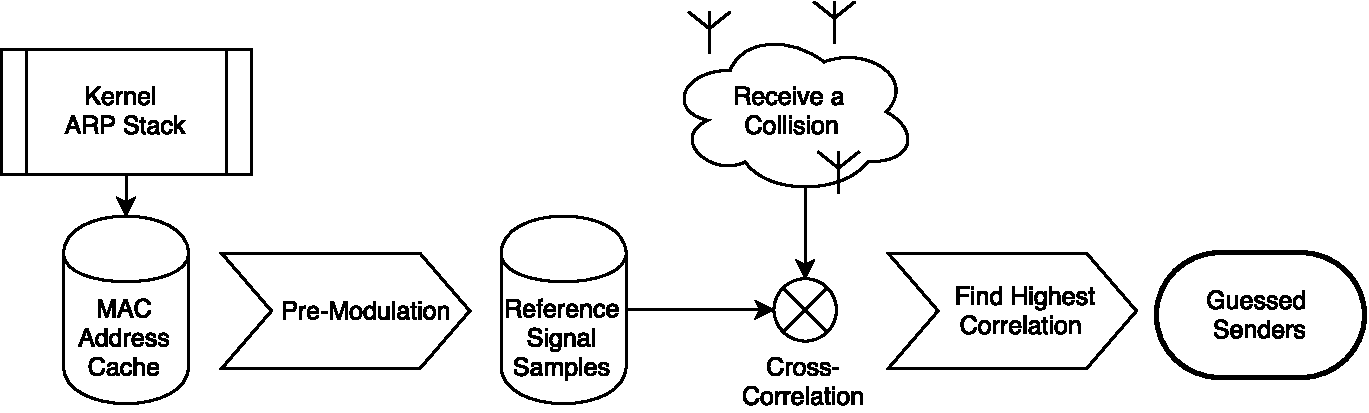
\includegraphics[width=\textwidth]{gfx/images/detector-block-design}
	\caption[High-Level Detector Design Schema]{High-Level Detector Design Schema}
	\label{fig:blockdesign}
\end{figure}

First of all, it is important to decide which \gls{MAC} addresses should be tested when processing a received collision. Since \gls{MAC} addresses are six byte values, there are $2^{48} \approx 3 \cdot 10^{14}$ possible instances. Although some \gls{MAC} addresses are invalid because the first three bytes denote the network interface vendor, and not all values have been issued\footnote{http://standards-oui.ieee.org/oui.txt}, there are still by far too many to try out all of them for every collision.

Instead, I make use of the operating system's \gls{ARP} stack. During normal network operation, the kernel already keeps a cache of \gls{MAC} addresses that have been observed. This list is perfectly suited for detecting senders, as it is quite likely that a collision occurs between senders that are already in the network for some time.\\

Next, I modulate IEEE 802.11 data frames for every cached \gls{MAC} address. These are used as reference signals for correlation with incoming collisions. Only a small chunk of the reference frames contains the \gls{MAC} address bits and is thus important for sender detection. I describe this region in detail in section \ref{sec:mac-periods}.

As mentioned in section \ref{sec:mac-and-phy}, there are different possibilities for frame encoding, namely the \gls{MCS}, the scrambler initialization, and the error-correcting convolutional encoding. Since the convolutional encoder uses a seven bit state, only the \gls{MAC} header field directly preceding the sender \gls{MAC} address is relevant here. That field is the destination \gls{MAC} address. In theory, all possible combinations could be modulated for the reference signals cache, however this would mean a total amount of  more than 130 thousand candidates for every \gls{MAC} address in the ARP pool. I evaluate the impact of these factors in chapter \ref{ch:evaluation}.

The amount of 130 thousand candidates, as mentioned above, is the product of three values: $ N_{\text{MCS}} $ denotes the possible Modulation and Coding Schemes, which are eight. $ N_{\text{Scrambler}} $ describes the available scrambler initialization values. For a seven bit state where the value zero is invalid \cite{ieee2012}, these are $ 2^7 - 1 = 127 $. $ N_{\text{Dest}} $ is the amount of possible states of the convolutional encoder, which are $ 2^7 = 128 $.

$$ N_{\text{MCS}} \cdot N_{\text{Scrambler}} \cdot N_{\text{Dest}} = 8 \cdot 127 \cdot 128 = 130 048 $$\vspace{0cm}

The modulation process comprises the following steps:

\begin{enumerate}
	\item Generate a \gls{MAC} header with appropriate sender and destination \gls{MAC} addresses
	\item Apply the scrambler with specific initialization value
	\item Run the convolutional encoder, which is deterministic
	\item Group bits and interleave symbols
	\item For a time-domain signal, apply \gls{IFFT} and add a cyclic prefix
\end{enumerate}

For correlation in the frequency domain, I omit step five. The \gls{FFT} has to be applied to the received collision signal in this case. I have done experiments with frequency-domain detection and show the results of these in section \ref{sec:freqd-correlation}.\\

When the receiver senses a transmission, I determine whether it is a collision using the IEEE 802.11 \gls{LTF}. Section \ref{sec:preamble-corr} gives details about this process. This also measures a possible delay between the two frames.

Upon noticing a collision, all reference samples are correlated with the signal under test. The correlations are then sorted in descending order by correlation magnitude. The highest correlations make up for the best guess which senders are subject to the collision.\\

It is worth noting that the output of this algorithm is always a probabilistic result. The technique will never detect senders with full confidence, but rather return a distribution of likelihood over the cache of reasonable \gls{MAC} addresses.


%% -----------------------------------------------------------------------------

\section{Detecting Frames and Collisions}\label{sec:preamble-corr}

A receiver captures a continuous stream of samples, generated by its \gls{ADC}. It is necessary to employ some mechanism to detect the start of a transmission. In regular operation, IEEE 802.11 receivers use the known preamble for this by correlating the \gls{LTF} to the incoming data in a sliding window approach \cite{perahia2013}.

This can be extended to recognizing collisions. Since the \gls{LTF} is designed in a way that it has low off-peak autocorrelation \cite{ieee2012}, there will be twice as many correlation peaks in a collision of two frames. The distance between the two \gls{LTF} pattern can even be used to calculate a possible delay between the two transmissions. An example of such correlation peaks in case of a collision is shown in Figure \ref{fig:preamble-corr}. Each frame causes two large spikes, and one spike with smaller magnitude. This is caused by the composition of the \gls{LTF} with two repetitions of a symbol, and a cyclic prefix of half the symbol size.\\

Knowing when the frames start is important for sender detection. Since the \gls{MAC} address is represented by only a small number of time-domain samples (see section \ref{sec:mac-periods}), it is vital to correlate the correct chunk of the signal.

\begin{figure}[H]
	\centering
	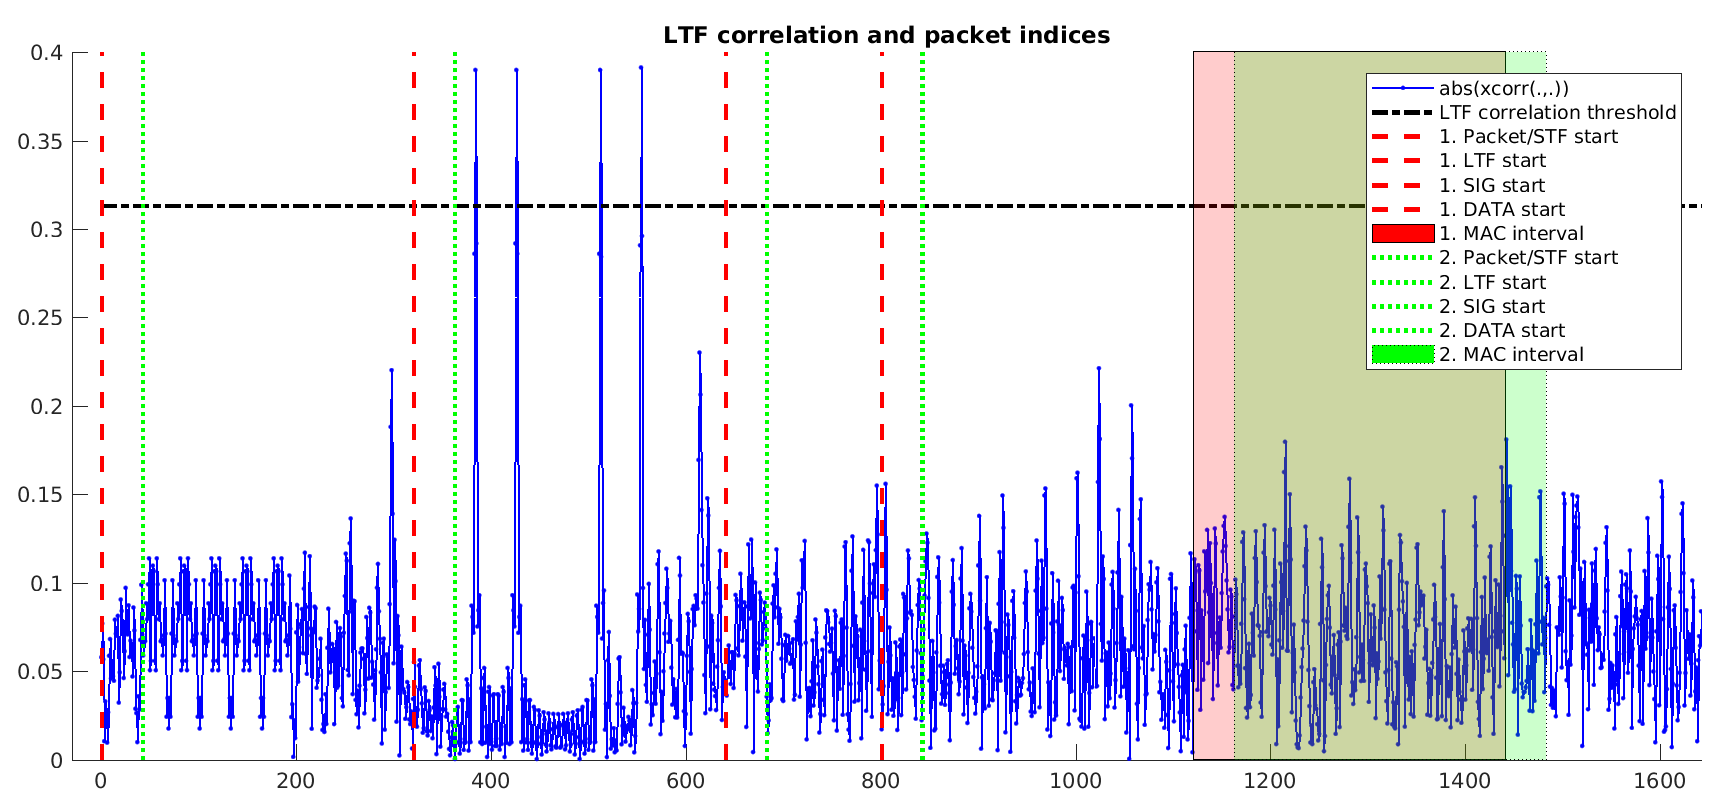
\includegraphics[width=\textwidth]{gfx/plots/preamble}
	\caption{Cross-Correlation of Collision Samples with Long Training Field}
	\label{fig:preamble-corr}
\end{figure}

Figure \ref{fig:preamble-corr} offers additional markers for the different signal fields as described in section \ref{sec:mac-and-phy}. Here, the symbols containing the \gls{MAC} address of the first frame begin after 1120 samples. The second \gls{MAC} address follows with an offset of about 40 samples.

When trying to decode these \gls{MAC} addresses, the correlations with the reference pool signals obviously have to be applied to the combined region of the first and second \gls{MAC} addresses. In this example, that would be all of the colored samples.


%% -----------------------------------------------------------------------------

\section{Periods Containing MAC Addresses}\label{sec:mac-periods}

Depending on the \gls{MCS}, the samples affected by different \gls{MAC} addresses start at different positions. The byte offset within the \gls{MAC} layer header remains the same. However, the amount of \gls{OFDM} symbols that need to be skipped before the beginning of the \gls{MAC} address, and the symbol count that has to be included to cover everything, change depending on the bit density.

Table \ref{tbl:sample-offsets} provides a summary of the various samples offsets for different \glspl{MCS}. These values are calculated assuming a sampling rate of 20 MHz. Since IEEE 802.11a/g channels have a passband bandwidth of 20 MHz, this is the minimum required sampling rate \cite{ieee2012}. However, some radios like the \gls{WARP} boards use a higher sampling rate of 40 MHz. In this case, all indices have to be doubled.\\

All frames begin with the preamble, specifically the Short and Long Training Fields, and the Signal Field. Both the \gls{STF} and \gls{LTF} have a duration of 8 $\mu$s. For the \gls{STF}, this is 10 repetitions of a 0.8 $\mu$s symbol. For the \gls{LTF}, there are two repetitions of a 3.2 $\mu$s symbol, and the 1.6 $\mu$s cyclic prefix. The Signal Field consists of one standard \gls{OFDM} symbol with cyclic prefix. That is 4 $\mu$s in the case of IEEE 802.11.

In total, the preamble takes 20 $\mu$s. At 20 MHz sampling rate, this results in $ 20 \cdot 10^{-6} s \cdot 20 \cdot 10^6 Hz= 400 $ samples. The Data Field thus start at sample index 401. Within that, the Service Field as well as the Frame Control and Duration \gls{MAC} header fields precede the \gls{MAC} addresses.\\

\begin{table}[ht]
	\centering
	\begin{tabular}{|p{2.5cm}|p{4.5cm}|p{4.5cm}|}
		\hline
		\textbf{MCS} & \textbf{Address 1 (Destination)} & \textbf{Address 2 (Sender)} \\ \hline
		0 & 561 - 720 & 721 - 880 \\ \hline
		1 & 481 - 640 & 561 - 720 \\ \hline
		2 & 481 - 560 & 561 - 640 \\ \hline
		3 & 401 - 560 & 481 - 560 \\ \hline
		4 & 401 - 480 & 481 - 560 \\ \hline
		5 & 401 - 480 & 401 - 480 \\ \hline
		6 & 401 - 480 & 401 - 480 \\ \hline
		7 & 401 - 480 & 401 - 480 \\ \hline
	\end{tabular}
	\caption{Sample Offsets of MAC Address Fields at Different MCSs}
	\label{tbl:sample-offsets}
\end{table}

\glspl{MCS} 0 and 2 have an important advantage. Only with these schemes does the above described region contain only the specific \gls{MAC} address, since the encoded bits per \gls{OFDM} symbol (24 for \gls{MCS} 0, and 48 for \gls{MCS} 1, as mentioned in Table \ref{tbl:mcs}) are integer multiples of the 48 bits \gls{MAC} address length. All other schemes contain additional data before the address, behind it, or in both positions.


%% -----------------------------------------------------------------------------

\section{Matlab Implementation}\label{sec:matlab-impl}

I built a proof of concept implementation of the presented technique in Matlab. Matlab was initially chosen for its large number of suitable toolboxes, and an existing implementation of the 802.11 MAC and PHY. It also allows to use \gls{WARP} \glspl{SDR}. The WARPLab 7.5.1 Matlab \gls{SDK}\footnote{http://warpproject.org/trac/wiki/WARPLab} provides easy-to-use high-level access to the radios. It was my preferred choice over the alternative of using Python and \gls{USRP} boards.\\

The Matlab code is structured into different sections. First, utility functions implement the generation of \gls{MAC} headers, modulating IEEE 802.11 data frames in the time domain, and choosing sender \gls{MAC} addresses randomly from a list. There are two different libraries used for modulation: MathWorks' WLAN System Toolbox\footnote{https://www.mathworks.com/products/wlan-system.html} as well as a custom IEEE 802.11 implementation developed at the \gls{SEEMOO} at TU Darmstadt.

A number of simulation scripts measure the detection algorithm's performance under simulated channel effects. The results of these are presented in chapter \ref{ch:evaluation}. A WARPLab script effectively does the same thing, but using three \gls{WARP} \glspl{SDR}. Finally, there are scripts that run a series of experiments varying certain parameters, save the data, and generate figures for evaluation.\\

The core of the Matlab implementation is cross-correlation. Using the Signal Processing Toolbox\footnote{https://www.mathworks.com/products/signal.html}, this can be done using the \texttt{xcorr} function. This function expects two complex sample series and returns a complex correlation vector and a real vector of offsets. The offsets range from the negative feature length up to the positive length. This is because the data series can be slided against each other in both directions. Using this function is similar to this example for an \gls{LTF} symbol:\\

\begin{lstlisting}[captionpos=b,caption={Cross-Correlation of an LTF Symbol},label=lst:xcorr]
[correlation, offset] = xcorr(rx, lts_t);
\end{lstlisting}

Analyzing the performance of my implementation revealed that most time was not spent on cross-correlation, but on the generation of the reference signal pool. I improved this code by applying the following optimizations.

First, since the sender detection only relies on correlating those samples that contain the \gls{MAC} address, as described in section \ref{sec:mac-periods}, most of the generated signal is discarded anyways. This means that it is unnecessary to spend valuable time on calculating the \gls{MAC} layer checksum, which is stored after the payload data. I simply use a placeholder value of 0x42424242 for the checksum. Furthermore, I do not generate the preamble, namely the Training and Signal Fields. This can be done by using the \texttt{wlanNonHTData} function from the WLAN System Toolbox. This function merely modulates the Data Field, in contrast to the \texttt{wlanWaveformGenerator} function.

Second, I store the reference signals in a cache that is reused in as many consecutive experiments as possible. All experiments were repeated for at least 100 runs. Since the reference pool remained the same for all repetitions, using a shared variable for the entire set almost cut the cost of a higher sample size to zero. This is because in relation to modulating a signal, calculating cross-correlations consumes several orders of magnitude less time (about 0.2 ms compared to 650 ms). This is good news because in a real-world application, the generation of reference signals can be done ahead of time, and signals under test do not have to be modulated since they are received already in the time domain.

Incorporating these optimizations reduced the runtime of the experiment varying the scrambler initialization, which is presented in section \ref{sec:ex-scrambler}, from an extrapolated 300 days to about 45 minutes on a consumer laptop. This not only allowed me to run the experiments at all, but also let me increase the number of repetitions, and therefore largely enhancing the sample size.\\

To simulate channel effects, different channel models from both the WLAN System Toolbox and the Communications System Toolbox \footnote{https://www.mathworks.com/products/communications.html} were used. The exact functions are described in the corresponding sections in chapter \ref{ch:evaluation}.\\

As addressed in section \ref{sec:preamble-corr}, it is necessary to detect the offset between two frames in a collision. This is done using the \texttt{meshgrid} Matlab function. Listing \ref{lst:meshgrid} shows an example of calculating the field indices of both collided frames. The code compares the signal-to-training symbol correlation with a defined threshold and finds peaks in the data. These are then grouped into four clusters. This effectively removes noise and measuring inaccuracies causing a spike to last for more than one sample. Due to the correlation of the preamble with one \gls{LTF} symbol, there should be two large and one small spike. This is because as described in section \ref{sec:mac-and-phy}, the \gls{LTF} comprises two symbol repetitions and a cyclic prefix of half a symbol length. Since the correlation threshold is chosen to be between the small and large spike, and assuming that exactly two frames collided, the expected amount of peaks is therefore four.

\begin{lstlisting}[captionpos=b,caption={Collision Offset Detection using Meshgrid},label=lst:meshgrid]
% Find peaks above a parametrized threshold
lts_peaks = find(abs(correlation) > LTS_CORR_THRESHOLD*max(abs(correlation)));

% Assuming two frames, there will be four high peaks
[~, C] = kmeans(lts_peaks', 4);
uniq_lts_peaks = sort(floor(C))';

% Select the best candidate correlation peak at LTS-payload boundary
[LTS1, LTS2] = meshgrid(uniq_lts_peaks, uniq_lts_peaks);
[lts_second_peak_index, y] = find(iswithin( ...
    LTS2-LTS1, ...
    length(lts_t)/1.2, ...
    length(lts_t)*1.2 ...
));

% Add 128 samples for the symbol itself (at 40 MHz)
ind2.sig = uniq_lts_peaks(max(lts_second_peak_index)) + 128;
ind2.ltf = ind2.sig - 320; % subtract LTF length
ind2.stf = ind2.ltf - 320; % subtract STF length
ind2.payload = ind2.sig + 160; % add 4us SIG field
ind1.sig = uniq_lts_peaks(min(lts_second_peak_index)) + 128;
ind1.ltf = ind1.sig - 320;
ind1.stf = ind1.ltf - 320;
ind1.payload = ind1.sig + 160;
\end{lstlisting}

The \texttt{meshgrid} function then calculates a two-dimensional table of all possible offsets between each two peaks. Using the \texttt{find} function, I look for offsets that equal the length of one training symbol with a 20 percent margin. This margin makes the algorithm a bit more reliable against slight timing imprecision. The offset between the collided frames is the delay between these symbol matches.

Lastly, the signal field sample indices are calculated as the last symbol's correlation peak plus the length of that symbol, which is 128 samples at 40 MHz sampling rate. Start indices of the \gls{LTF}, \gls{STF}, and Data Field are deduced accordingly.\\

The indices are stored in a structure, which is later used to cut out the samples containing the sender's MAC address. That set is determined as the start of the address in the first frame until the end of the address in the second frame. Especially on real hardware, this allows to mitigate possible delays and offset between the frames.

%% -----------------------------------------------------------------------------

\chapter{Evaluation}\label{ch:evaluation}
\glsresetall % Resets all acronyms to not used

In this chapter, the proposed technique for detecting sender \gls{MAC} addresses during collisions is evaluated using several simulations as well as experiments on \gls{WARP} \glspl{SDR}.

Possible questions and problems include the fact, that with higher \glspl{MCS}, there could be not enough samples to correlate the rather short 6 byte \gls{MAC} address. Another interesting issue is the accuracy of the algorithm with increasing amounts of noise and fading.


%% -----------------------------------------------------------------------------

\section{Frequency-Domain Correlation}\label{sec:freqd-correlation}

During the implementation of the \gls{MAC} address detection technique, I tried using cross-correlation in the frequency-domain. This means that instead of calculating the similarity between samples, complex symbols are correlated without mapping them into the time-domain. With this approach, the Fourier transform must be applied to the received signal.

It turns out to be at least very difficult, if not impossible, to detect senders in case of a collision with frequency-domain correlation. The reason for that is phase shift due to path delays. When a signal is received with an offset in the time-domain, the constellation is changed in the frequency-domain. This can be shown using the Fourier transform equation:

$$ F(f) = \int_{-\infty}^{\infty} s(t) \cdot e^{-2 \pi i f t} dt $$\vspace{0cm}

Here, $ i $ is the imaginary unit, $ F(f) $ is the Fourier transform at frequency $ f $, and $ s(t) $ is the time-domain signal depending on $ t $. A time offset can now be expressed as $ t + \Delta $. Standard power laws then show that this offset introduces a constant multiplication factor on $ F(f) $, depending on $ \Delta $.

$$ F(f) = \int_{-\infty}^{\infty} s(t + \Delta) \cdot e^{-2 \pi i f \cdot (t + \Delta)} dt = \int_{-\infty}^{\infty} s(t + \Delta) \cdot e^{-2 \pi i f t} \cdot e^{-2 \pi i f \Delta} dt = $$
$$ = e^{-2 \pi i f \Delta} \cdot \int_{-\infty}^{\infty} s(t + \Delta) \cdot e^{-2 \pi i f t} dt $$\vspace{0cm}

Since both $ s(t) $ and $ F(f) $ are complex functions, this multiplication is a rotation, or phase shift, in the complex constellation plane. Furthermore, the rotation is different for different frequencies $ f $.

This leads to a received constellation similar to that shown in figure \ref{fig:freqd-corr}. To create this figure, I applied a Rayleigh channel \cite{sklar1997} to a simulated collision signal, introducing a delay of a few nanoseconds. The signals are modulated with \gls{BPSK}, so ideally the only constellation points should be $ 1 $ and $ -1 $. However, due to the above described rotation, the constellation is basically a circle.

\begin{figure}[ht]
	\centering
	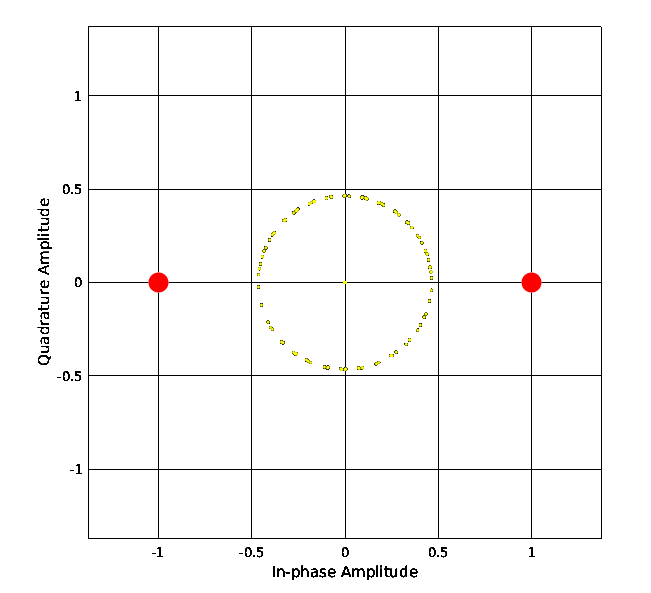
\includegraphics[width=8cm]{gfx/images/freqd-correlation}
	\caption{Cross Correlation of Frequency-Domain Symbols after Channel}
	\label{fig:freqd-corr}
\end{figure}

This kind of path effects is not at all unusual in a IEEE 802.11 transmission. Under normal circumstances, the known preamble is used to calculate the inverted channel matrix of the path effects, as mentioned in section \ref{sec:multipath}.

When receiving a collision, there is however not only one preamble. Instead, the preambles of two different frames, which experienced different path effects, are added together. Since the preambles themselves are designed to have a low off-peak autocorrelation \cite{ieee2012}, it is not easily possible to separate the two channel effects from each other. Therefore, I can not reverse the phase shift introduced on the \gls{OFDM} symbols containing the \gls{MAC} address.

As expected, experiments with cross-correlation in the frequency-domain without channel equalization were unsuccessful. I therefore disregarded this approach.


%% -----------------------------------------------------------------------------

\section{Time-Domain Correlation}

The experiments I did using time-domain cross-correlation are devided in two groups. First, I used Matlab to simulate different field variations and channel effects. Second, I used WARP boards to try the approach in a real-world scenario. The results of these experiments are summarized in the following sections.

When correlating time-domain samples, I always pre-generated reference samples and calculated the correlation only for the subset of samples that contains the \gls{MAC} address. Section \ref{sec:mac-periods} describes which period of the signal this is.\\

Reference signals are modulated until just after the \gls{IFFT} and adding of cyclic prefix. For the simulations, I used a sampling rate of 20 MHz, which is the default output of the Matlab WLAN System Toolbox. The WARP boards use a sampling frequency of 40 MHz however, so for these experiments I used interpolation to double the rate.

All experiments used realistic real-world \gls{MAC} addresses, as described in section \ref{sec:real-world-macs}.


%% -----------------------------------------------------------------------------

\section{Real-World MAC Addresses}\label{sec:real-world-macs}

\gls{MAC} addresses are 6 byte numbers, where the first 3 bytes are a vendor prefix, identifying the company that built the network interface. The remaining 3 bytes are a unique identifier for the specific hardware.

After initial tries with some artificial \gls{MAC} addresses in the form of \texttt{AB:CD:EF:12:34:56}, I switched to using a sample set of real-world \gls{MAC} addresses. This allowed for a closer simulation of an actual use-case for sender detection.\\

I collected 64 \gls{MAC} addresses from devices that were connected to the wireless university eduroam network. The gathering was done in the afternoon on a weekday. I used airodump from the \texttt{aircrack-ng} software suite to dump all \gls{MAC} addresses on the network into a file. The actual command looked like this:

\begin{lstlisting}[captionpos=b,caption={Capture Real-World MAC Addresses},label=lst:airodump]
airmon-ng start wlp0s20u1
airodump-ng --essid eduroam -a -o csv -w mac-addresses-eduroam.csv wlp0s20u1mon
\end{lstlisting}

It is important to have the wireless network interface set to promiscuous mode. This mode instructs the driver to hand all received frames to the kernel. Otherwise, only frames that are addressed to or coming from the local station are gathered, while the rest is filtered. This would mean that only the router's and the station's own \gls{MAC} address would be cached.

In a possible real-time usage scenario of the sender detection algorithm, it would also be important to use promiscuous mode in order to collect all \gls{MAC} addresses. These are the addresses for which reference signals need to be modulated and cached.


%% -----------------------------------------------------------------------------

\section{Modulation and Coding Schemes}

Intuitively, the overall sender detection accuracy should decrease for higher \glspl{MCS}. Firstly, with a higher \gls{MCS} there are more payload bits encoded in every \gls{OFDM} symbol, as described in table \ref{tbl:mcs}. This means that when applying cross-correlation, the \gls{OFDM} symbol contains random data from the \gls{MAC} header before and after the sender \gls{MAC} address. Due to the nature of \gls{OFDM}, it is not possible to limit correlation to only a fraction of the symbol in the time-domain.

Secondly, the higher constellation itself, which comes with higher \gls{MCS}, means that payload data gets mapped to complex points in the constellation plane that are less distinct from each other. Therefore, different data can be more similar under cross-correlation, making it harder to detect senders in the time-domain.\\

To evaluate the detection algorithm's performance, I measured the correctness of detected \gls{MAC} addresses for each of the 8 available \glspl{MCS}. For every \gls{MCS}, 1000 runs were performed. The results are the stacked sums of times where a completely correct pair of senders were guessed, times where only one of the senders was correct, and the amount of failures, in the sense of both addresses being incorrect.

Figure \ref{fig:vary_mcs} is the resulting plot. Different \glspl{MCS} are spread out on the x axis. The stacked bars show the amount of experiments for each result category as described above. As expected, the detection accuracy decreases for higher \glspl{MCS}. It is worth mentioning that for low \glspl{MCS}, the performance is very good, better than I expected. Furthermore, it seems to decrease exponentionally, but to justify this more data would be needed.

\begin{figure}[H]
	\centering
  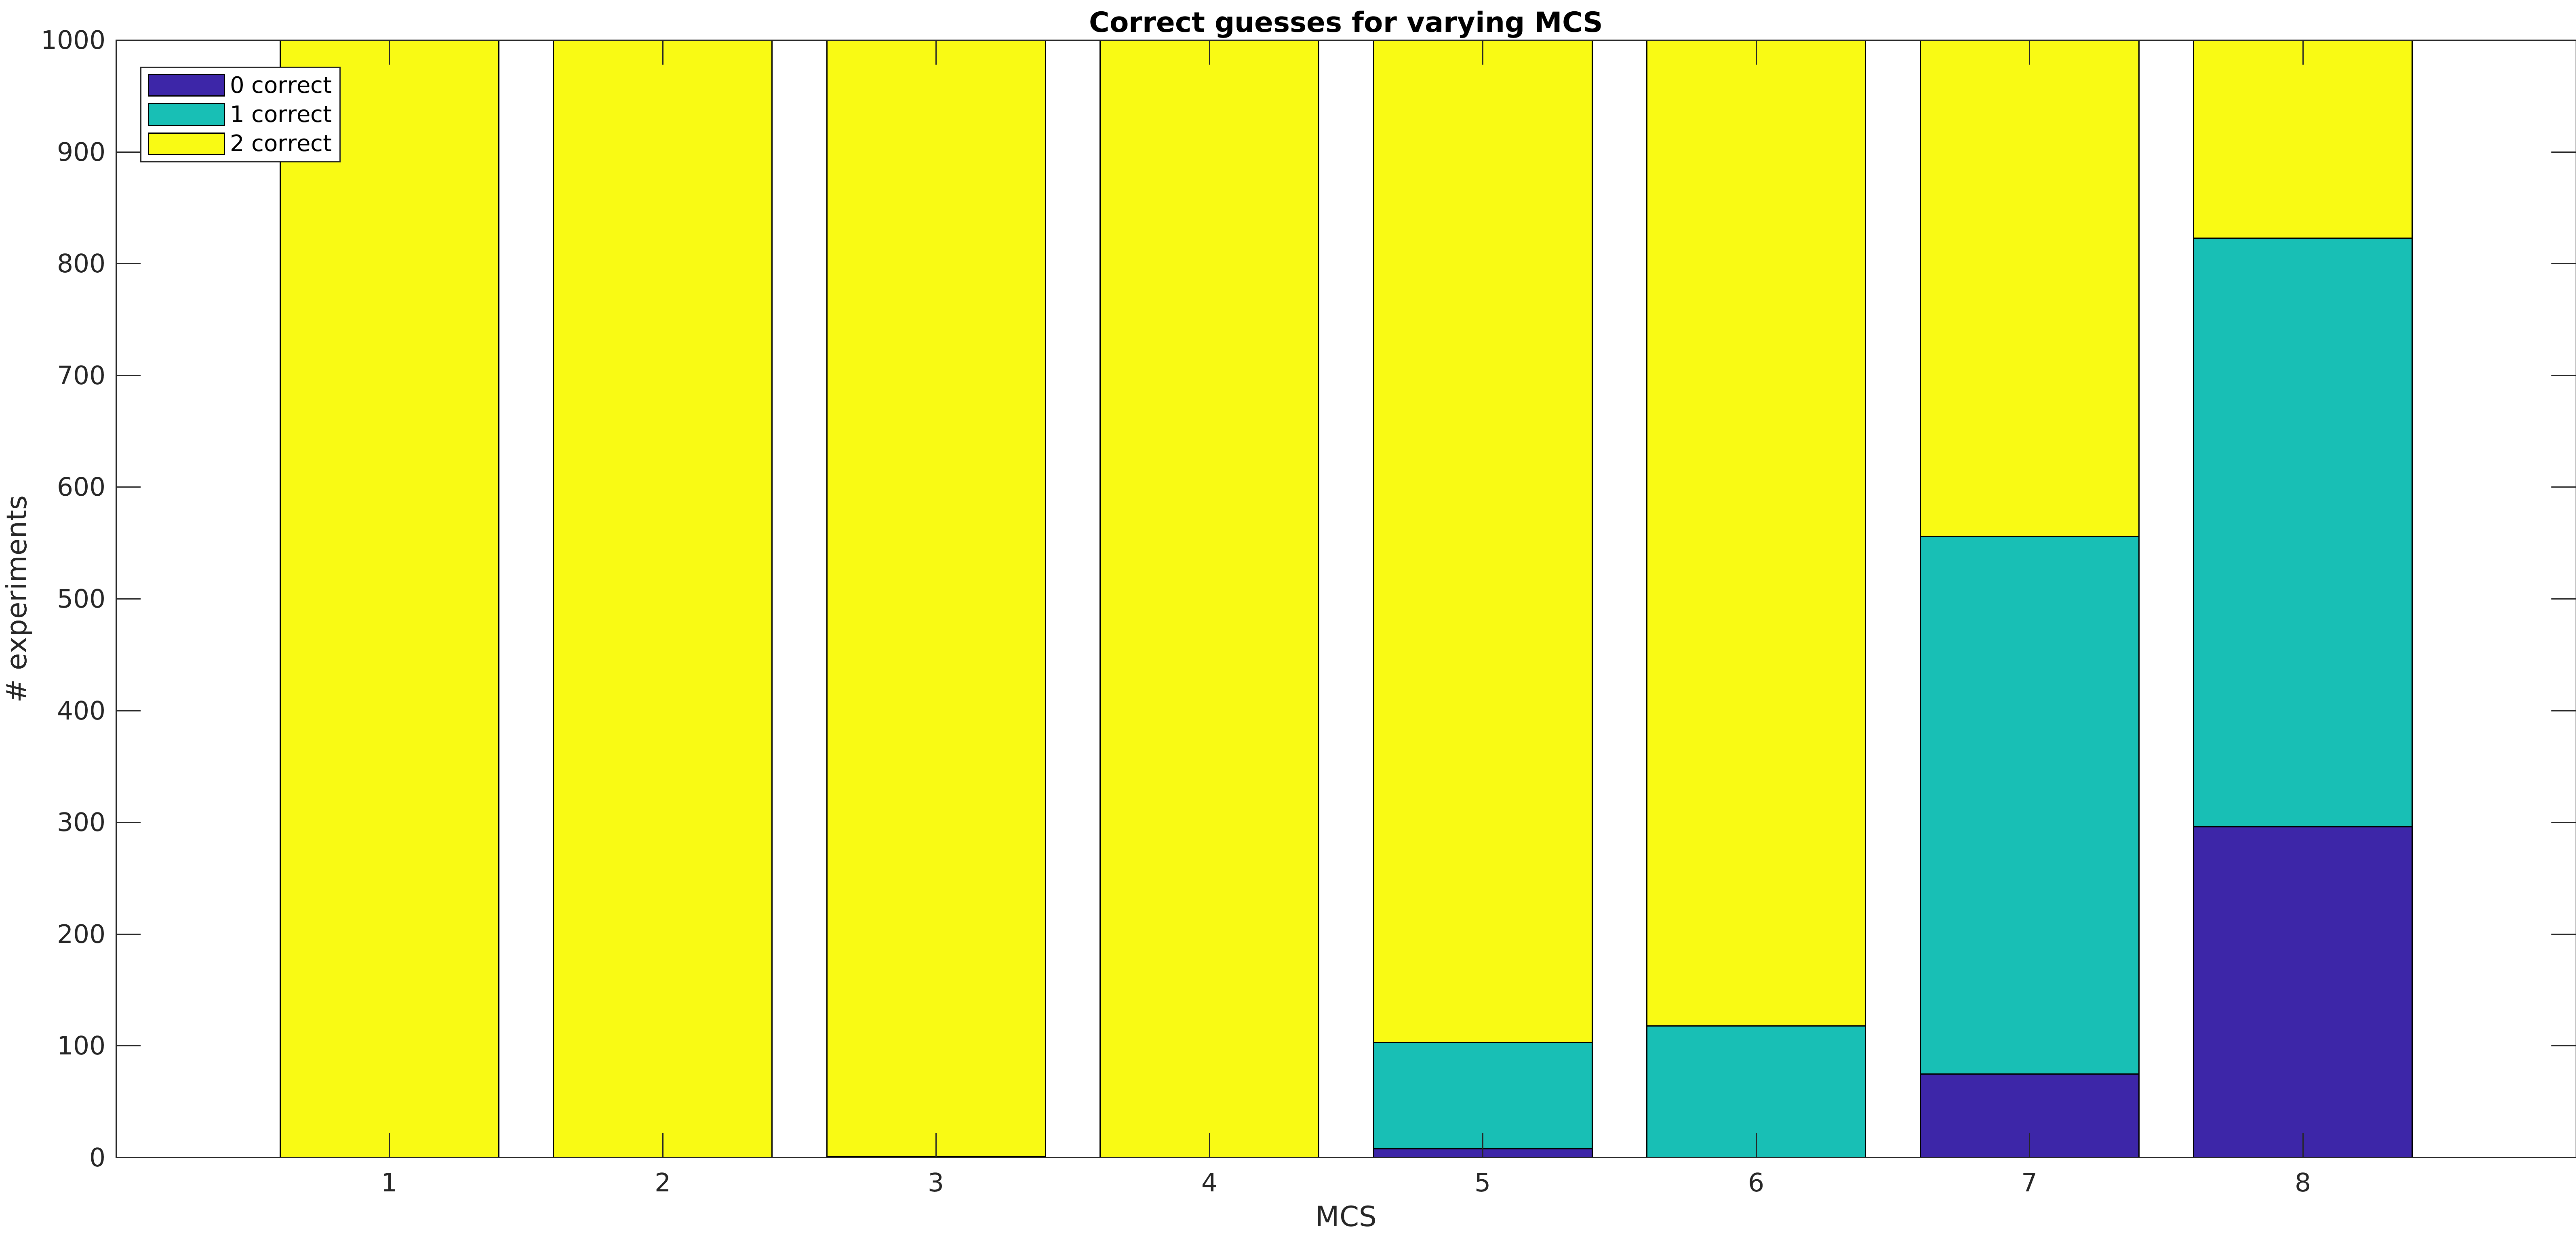
\includegraphics[width=\textwidth]{gfx/plots/vary_mcs-20170608-1859-num_correct-64_addresses-1000_experiments.png}
	\caption{Results: Varying MCS for 1000 Runs}
	\label{fig:vary_mcs}
\end{figure}


%% -----------------------------------------------------------------------------

\section{Scrambler Initialization}\label{sec:ex-scrambler}

As described in section \ref{sec:mac-and-phy}, the \gls{MAC} layer payload data is scrambled before any modulation on the physical layer is applied. The scrambling uses a 7 bit state register, where 0 is no valid state. Therefore, 127 unique scrambler initialization values are possible.

If the scrambler initialization is important for the sender detection technique, specifically if the modulated reference signals must use the same initialization as the received frames, the amount of possible values linearly scales the algorithm's complexity. That is, for every cached \gls{MAC} address, \gls{MCS} et cetera all scrambler initializations must be modulated and correlated. It is therefore very interesting to know whether that is the case, or whether the scrambler alternatively does not affect detection quality.\\

Figure \ref{fig:vary_scrambler} shows the detection performance for different scrambler initializations over 1000 experiments. The data is presented the same way as in the previous section as stacked bar plots denoting the amount of runs with 0, 1, and 2 corrects guesses. For all experiments, the \gls{MCS} 0 was used. While the simulated received frame was modulated with scrambler initialization 1, correlation was calculated against 127 reference signals with different scrambler values.

The results show that indeed the scrambler initialization is very important for detection quality. While the performance is very good for the correct initialization value 1, for all other values the accuracy is low. However, related research mentions that some network interfaces seem to not choose the scrambler initialization at random \cite{noubir2016}, contradictory to the IEEE 802.11 standard. These devices use a static initialization for every frame, or increment the value after every transmission. This could be exploited by limiting the reference signals to such that are expected in the current network, therefore avoiding time spent on correlations that are unpromising. Since the \gls{MAC} addresses of stations in the network are cached, the interface types and vendors are known. This could lead to some interesting future work.

\begin{figure}[H]
	\centering
	% uncomment the following line to recompile the figure when it changes otherwise a cached version is used
	%\tikzset{external/remake next}
	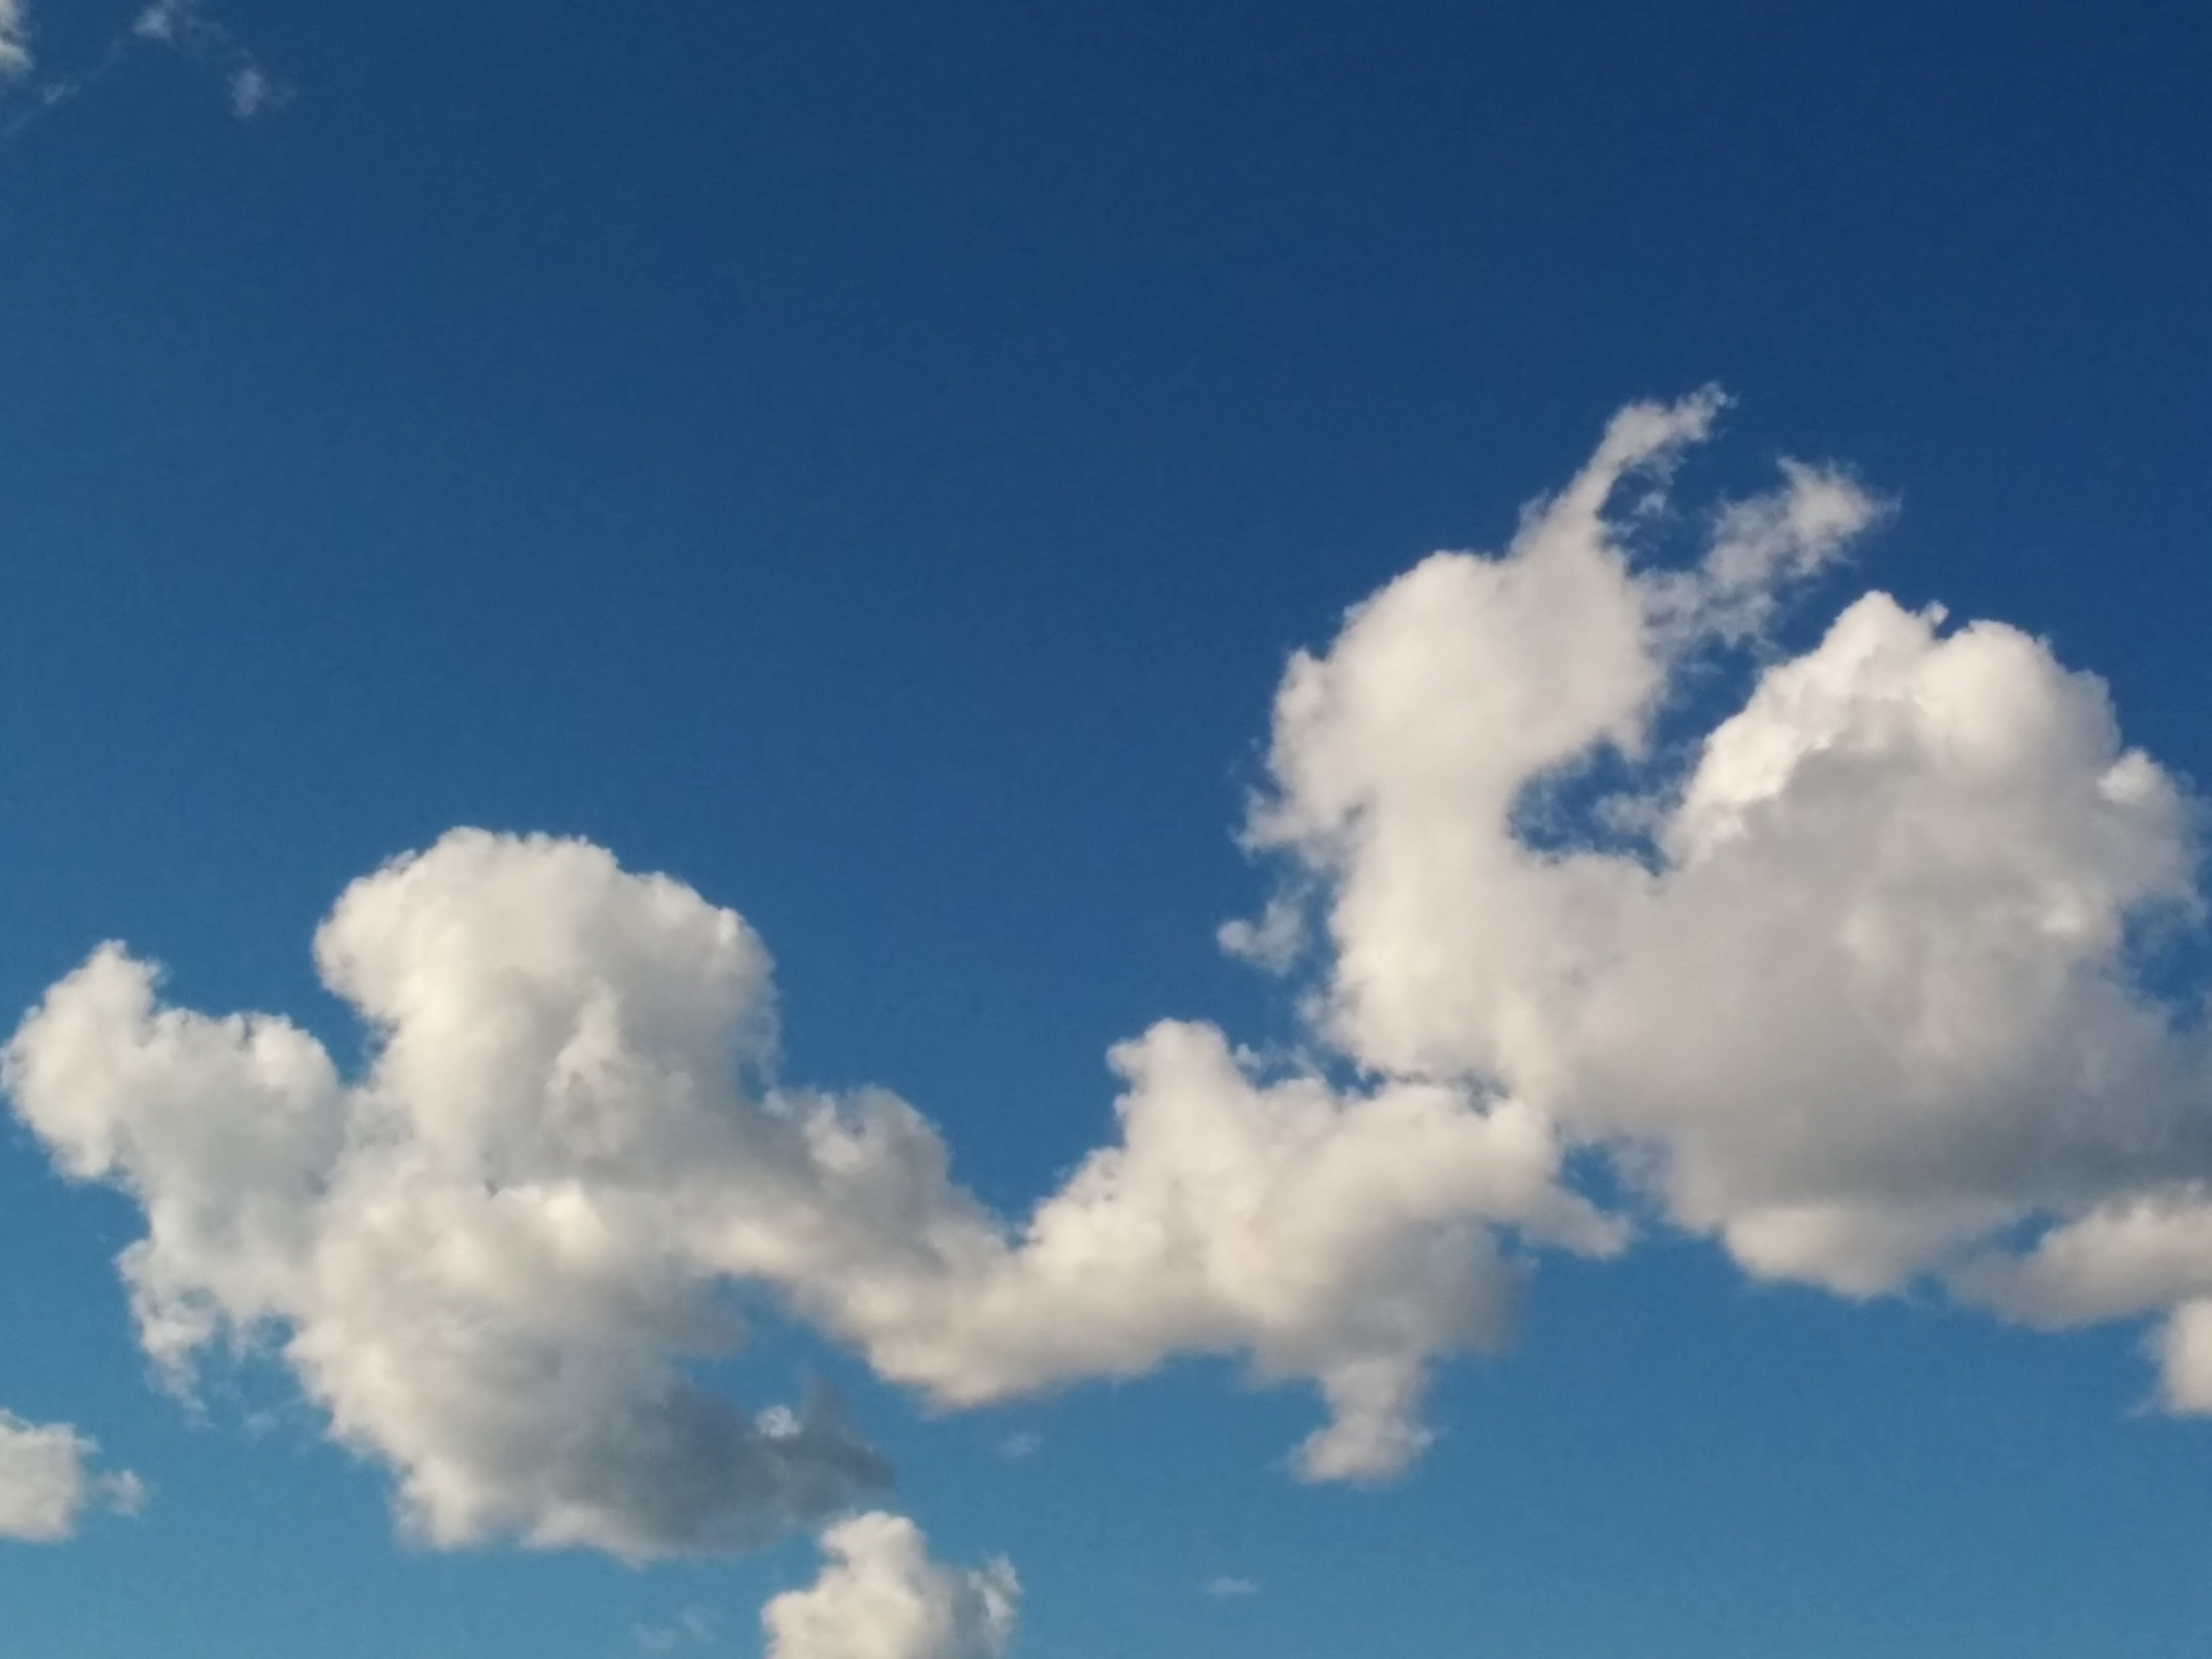
\includegraphics[width=0.9\textwidth,height=5cm]{gfx/images/stock-clouds}
	\caption[Results: Varying Scrambler Initialization for 1000 Experiments]{Results: Varying Scrambler Initialization for 1000 Runs at MCS 0}
	\label{fig:vary_scrambler}
\end{figure}


%% -----------------------------------------------------------------------------

\section{Preceding Data Variations}\label{sec:ex-destination}

Similar to the scrambler initialization, the \gls{MAC} header field preceding the sender \gls{MAC} address could also influence detection quality. This is due to the convolutional encoder as described in section \ref{sec:mac-and-phy}. The field before the sender \gls{MAC} address in a data frame is the destination \gls{MAC} address. In the following experiment, I measured to which extent the value of the destination address affects the accuracy of my detection technique.\\

Figure \ref{fig:vary_dest} shows the results in the same way as for the previous figures. Since the convolutional encoder uses a 7 bit state, only the last 7 bits of the destination \gls{MAC} address matter. After these last 7 bits, the register is synchronized to the same state, regardless of the preceding first 41 bits of the address. This makes up for a total of 128 different values that are evaluated with 1000 experiments each. As for the scrambler initialization, the experiments are done at \gls{MCS} 0.

\begin{figure}[H]
	\centering
	% uncomment the following line to recompile the figure when it changes otherwise a cached version is used
	%\tikzset{external/remake next}
	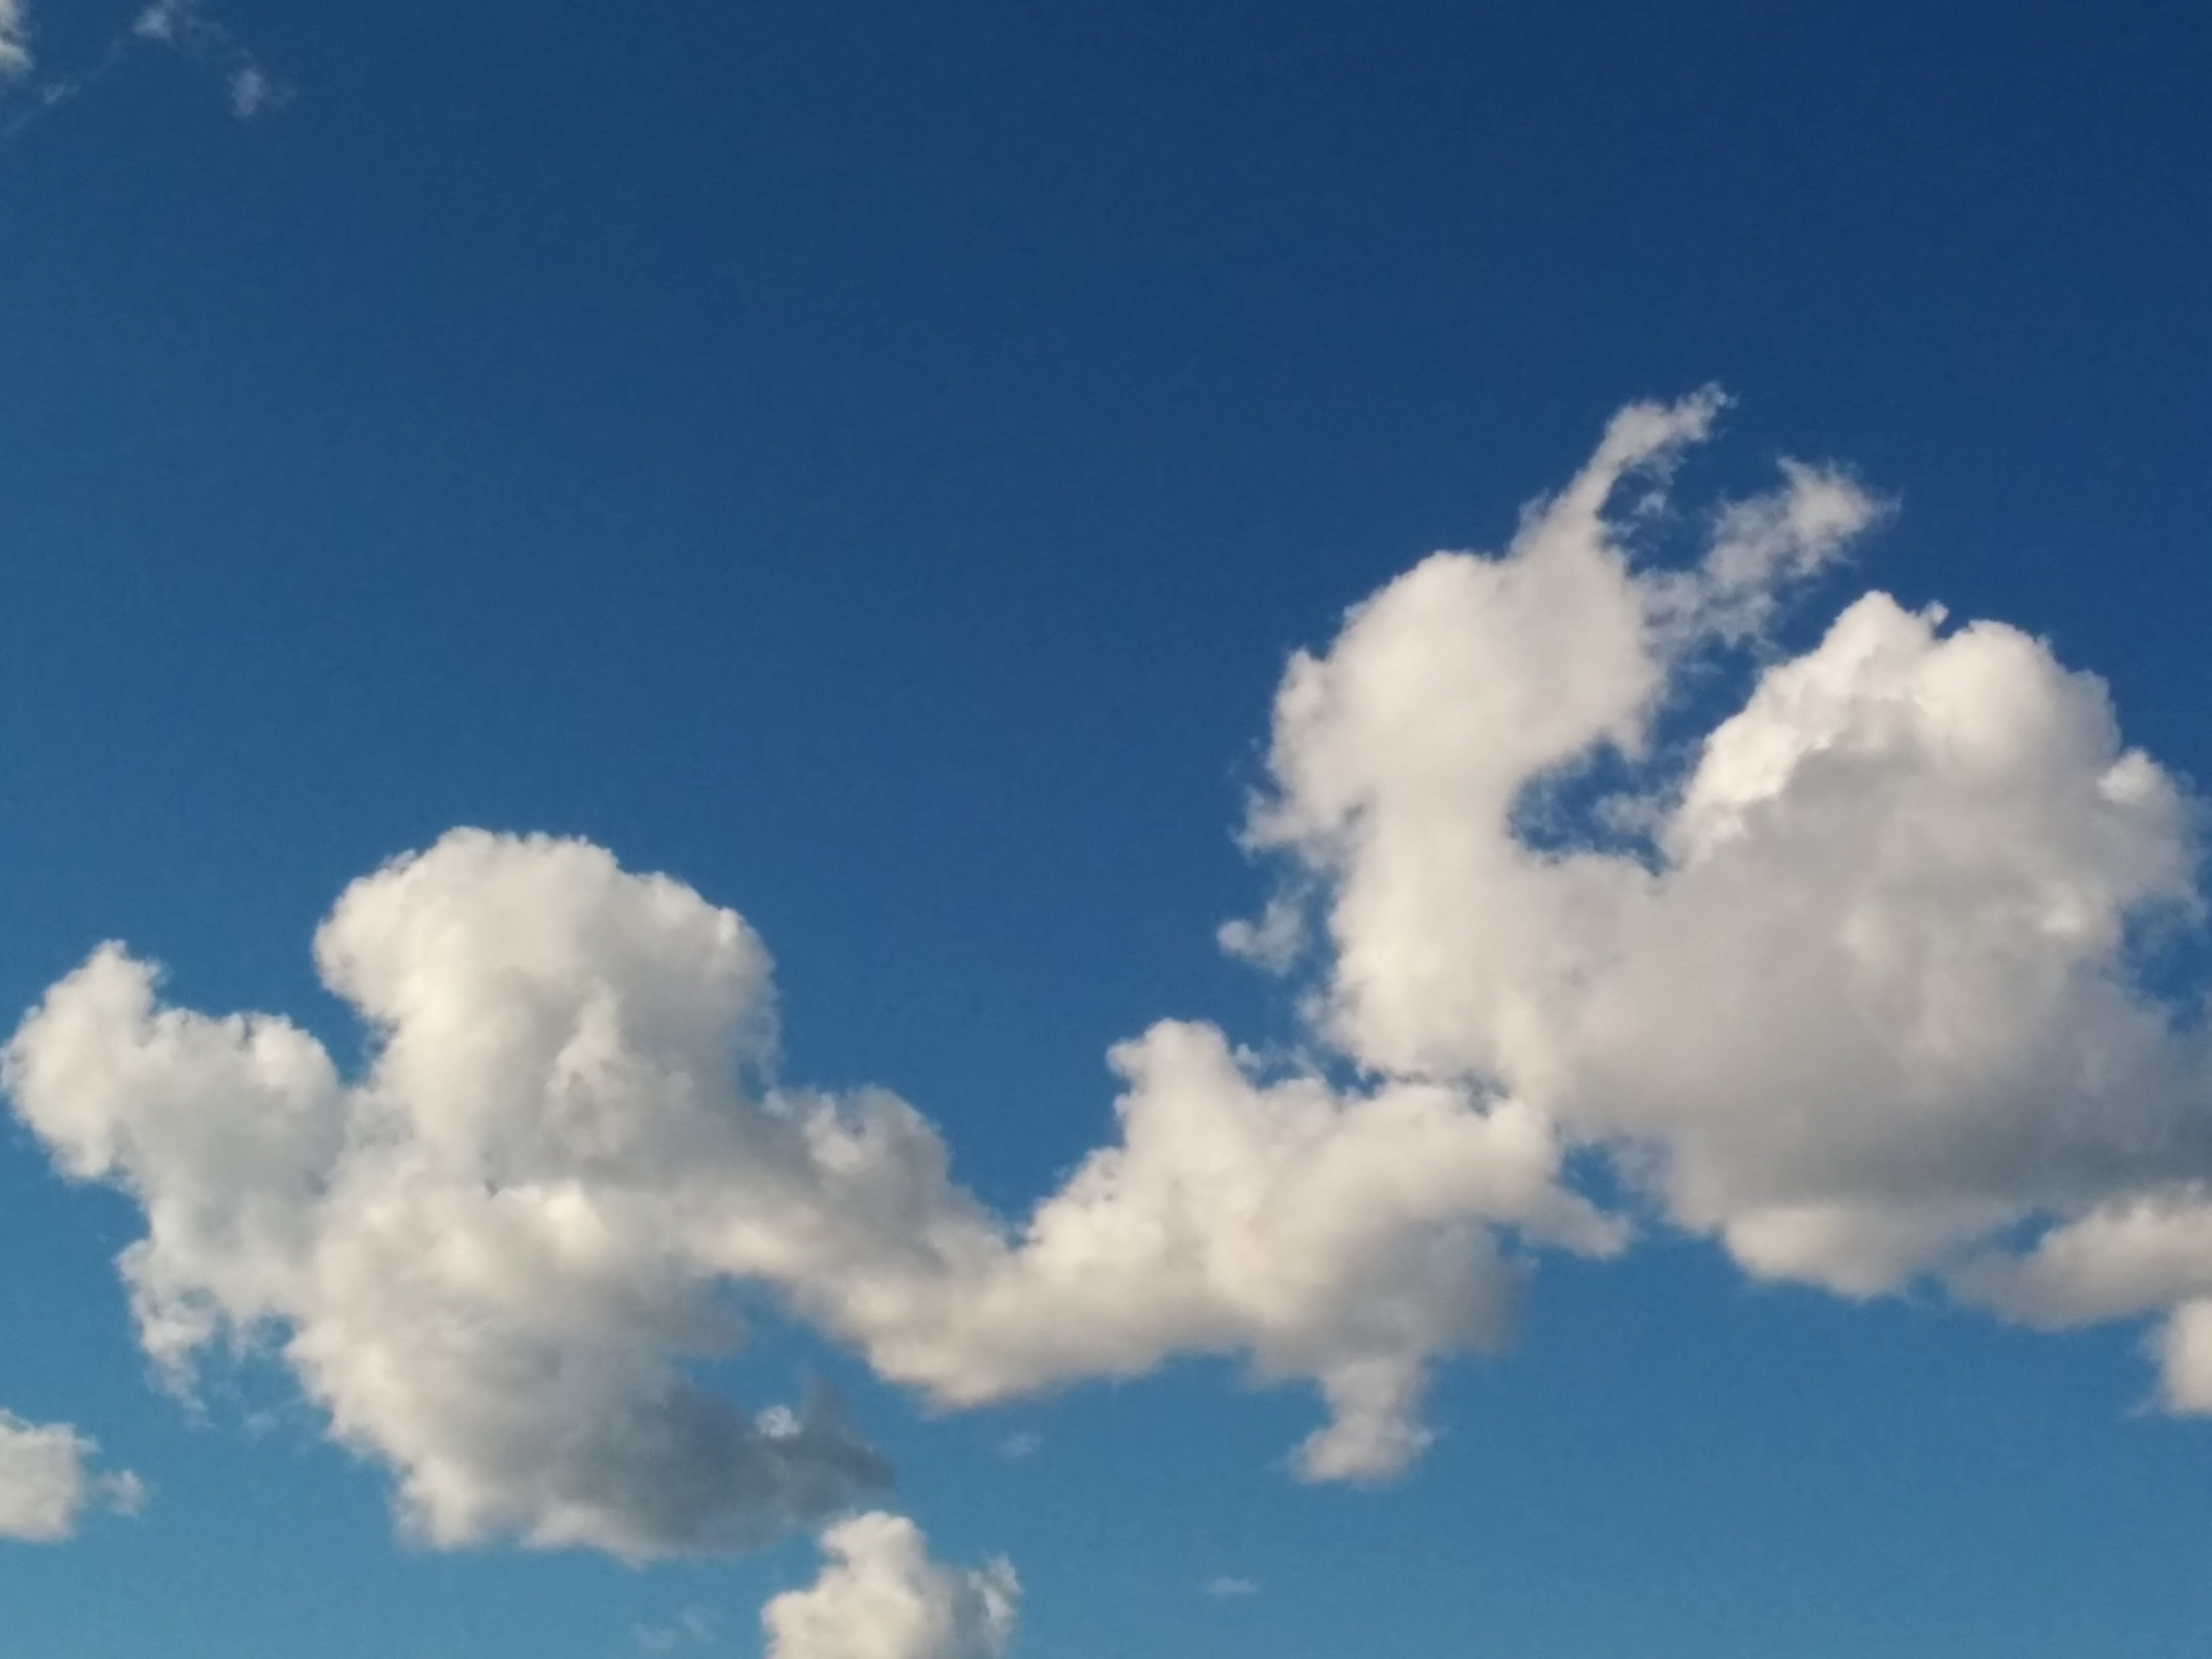
\includegraphics[width=0.9\textwidth,height=5cm]{gfx/images/stock-clouds}
	\caption[Results: Varying Destination \gls{MAC} Address for 1000 Experiments]{Results: Varying Destination \gls{MAC} Address for 1000 Experiments at MCS 0}
	\label{fig:vary_dest}
\end{figure}

It turns out that unlike the scrambler initialization, preceding payload data does not really have a measurable effect. Detection quality is comparable regardless of the trailing bits of the \gls{MAC} address. I discuss possible reasons for this in section \ref{sec:detection-quality}. An important implication of this result is that it is not necessary to check all 128 possible encoder states for every collision in real-time, which would be another linear scaling factor for the computational complexity of the algorithm.


%% -----------------------------------------------------------------------------

\section{Channel Models}

So far, all experiments were done in simulations with an ideal channel, meaning there were no path effects such as multi-path fading or attenuation. As this is not very realistic, I will evaluate performance under various channel models in this section.\\

Using Matlab, there are different models available that could be applied. On the one hand, the Communications System Toolbox comes with \texttt{stdchan}, which supports the \texttt{802.11g} and \texttt{802.11g} channel types. These are suited quite well for this scenario. The channel models requires some parameters, including the sampling frequency, Doppler spread, and \gls{RMS} delay spread $ t_{RMS} $. The delay spread was varied from 100 ns to 500 ns in steps of 50 ns. The usage of the stdchan filter is illustrated by listing \ref{lst:stdchan}:

\begin{lstlisting}[captionpos=b,caption={Matlab stdchan Channel Model},label=lst:stdchan]
tmrs = ...;
fs = 20e6; % Hz Sampling Frequency
fd = 10; % Hz Doppler spread
chan = stdchan(1/fs, fd, '802.11g', trms);
rx = filter(chan, tx);
\end{lstlisting}

The results of this experiment are shown in figure \ref{fig:vary_trms}. For every \texttt{trms} value, 1000 runs were performed. The process was repeated for all eight \glspl{MCS}.

On the other hand, the WLAN Systems Toolbox comes with a number of specifically drafted IEEE 802.11 channel models. These are designed according to the IEEE 802.11 standard models described in the specification \cite{ieee2012}. There are 6 models (A to F), of which I used the following three:

\begin{itemize}
	\item \textit{Model B}: typical large open space and office environments, no line-of-sight, 100 ns \gls{RMS} delay spread
	\item \textit{Model D}: large open space (indoor and outdoor), line-of-sight conditions, 140 ns \gls{RMS} delay spread
	\item \textit{Model E}: typical large open space (indoor and outdoor), no line-of-sight, 250 ns \gls{RMS} delay spread
\end{itemize}

I use the \texttt{wlanTGnChannel} class. Technically, this channel is designed to be used with IEEE 802.11 n high-throughput networks. However, the class supports configuration of \gls{MIMO} streams. I set those to 1 antenna for transmission and reception, respectively. This should provide appropriate conditions for \gls{SISO} 802.11 a/g networks.

The channel is used with Matlab code similar to listing \ref{lst:tgn}. As for the \texttt{stdchan} invocation, the sampling rate must be passed to the function. I use path-loss and shadowing for fading, and configure \gls{SISO}.

\begin{lstlisting}[captionpos=b,caption={Matlab wlanTGnChannel Simulation},label=lst:tgn]
model = ...; % 'Model-B', 'Model-D', etc.
tgnchan = wlanTGnChannel( ...
        'SampleRate', 20e6, ... % Hz
        'LargeScaleFadingEffect', 'Pathloss and shadowing', ...
        'NumTransmitAntennas', 1, 'NumReceiveAntennas', 1, ... % SISO
        'DelayProfile', model);
rx = tgnchan(tx);
\end{lstlisting}

The results of the experiments are shown in figure \ref{fig:vary_tgn}. For each of the three channel models, 1000 runs were performed at each \gls{MCS}.

\begin{figure}[p]
	\centering
	\setlength\figureheight{3cm}
	\setlength\figurewidth{0.40\textwidth}
	\begin{tabular}{cc}
		% uncomment the following line to recompile the figure when it changes otherwise a cached version is used
		%\tikzset{external/remake next}
		\subfloat[MCS 0]{% This file was created by matlab2tikz.
%
%The latest updates can be retrieved from
%  http://www.mathworks.com/matlabcentral/fileexchange/22022-matlab2tikz-matlab2tikz
%where you can also make suggestions and rate matlab2tikz.
%
\definecolor{mycolor1}{rgb}{0.24220,0.15040,0.66030}%
\definecolor{mycolor2}{rgb}{0.09640,0.75000,0.71204}%
\definecolor{mycolor3}{rgb}{0.97690,0.98390,0.08050}%
%
\begin{tikzpicture}[%
font=\footnotesize
]

\begin{axis}[%
width=0.951\figurewidth,
height=\figureheight,
at={(0\figurewidth,0\figureheight)},
scale only axis,
bar width=0,
xmin=5e-08,
xmax=5.5e-07,
xlabel style={font=\color{white!15!black}},
xlabel={$\text{802.11g stdchan: t}_\text{R}\text{MS in seconds}$},
ymin=0,
ymax=10,
ylabel style={font=\color{white!15!black}},
ylabel={\# experiments},
axis background/.style={fill=white},
title style={font=\bfseries},
title={MCS 0},
legend style={legend cell align=left, align=left, draw=white!15!black},
clip mode=individual,transpose legend,legend columns=2,legend style={at={(0,1)},anchor=north west,draw=black,fill=white,legend cell align=left}
]
\addplot[ybar stacked, fill=mycolor1, draw=black, area legend] table[row sep=crcr] {%
1e-07	0\\
1.5e-07	0\\
2e-07	0\\
2.5e-07	0\\
3e-07	0\\
3.5e-07	0\\
4e-07	0\\
4.5e-07	0\\
5e-07	0\\
};
\addplot[forget plot, color=white!15!black] table[row sep=crcr] {%
5e-08	0\\
5.5e-07	0\\
};
\addlegendentry{0 correct}

\addplot[ybar stacked, fill=mycolor2, draw=black, area legend] table[row sep=crcr] {%
1e-07	5\\
1.5e-07	3\\
2e-07	8\\
2.5e-07	4\\
3e-07	6\\
3.5e-07	7\\
4e-07	8\\
4.5e-07	7\\
5e-07	7\\
};
\addplot[forget plot, color=white!15!black] table[row sep=crcr] {%
5e-08	0\\
5.5e-07	0\\
};
\addlegendentry{1 correct}

\addplot[ybar stacked, fill=mycolor3, draw=black, area legend] table[row sep=crcr] {%
1e-07	5\\
1.5e-07	7\\
2e-07	2\\
2.5e-07	6\\
3e-07	4\\
3.5e-07	3\\
4e-07	2\\
4.5e-07	3\\
5e-07	3\\
};
\addplot[forget plot, color=white!15!black] table[row sep=crcr]  &
		\subfloat[MCS 1]{% This file was created by matlab2tikz.
%
%The latest updates can be retrieved from
%  http://www.mathworks.com/matlabcentral/fileexchange/22022-matlab2tikz-matlab2tikz
%where you can also make suggestions and rate matlab2tikz.
%
\definecolor{mycolor1}{rgb}{0.24220,0.15040,0.66030}%
\definecolor{mycolor2}{rgb}{0.09640,0.75000,0.71204}%
\definecolor{mycolor3}{rgb}{0.97690,0.98390,0.08050}%
%
\begin{tikzpicture}[%
font=\footnotesize
]

\begin{axis}[%
width=0.951\figurewidth,
height=\figureheight,
at={(0\figurewidth,0\figureheight)},
scale only axis,
bar width=0,
xmin=5e-08,
xmax=5.5e-07,
xlabel style={font=\color{white!15!black}},
xlabel={$\text{802.11g stdchan: t}_\text{R}\text{MS in seconds}$},
ymin=0,
ymax=10,
ylabel style={font=\color{white!15!black}},
ylabel={\# experiments},
axis background/.style={fill=white},
title style={font=\bfseries},
title={MCS 1},
legend style={legend cell align=left, align=left, draw=white!15!black},
clip mode=individual,transpose legend,legend columns=2,legend style={at={(0,1)},anchor=north west,draw=black,fill=white,legend cell align=left}
]
\addplot[ybar stacked, fill=mycolor1, draw=black, area legend] table[row sep=crcr] {%
1e-07	0\\
1.5e-07	0\\
2e-07	0\\
2.5e-07	1\\
3e-07	4\\
3.5e-07	2\\
4e-07	6\\
4.5e-07	5\\
5e-07	4\\
};
\addplot[forget plot, color=white!15!black] table[row sep=crcr] {%
5e-08	0\\
5.5e-07	0\\
};
\addlegendentry{0 correct}

\addplot[ybar stacked, fill=mycolor2, draw=black, area legend] table[row sep=crcr] {%
1e-07	6\\
1.5e-07	6\\
2e-07	10\\
2.5e-07	7\\
3e-07	5\\
3.5e-07	7\\
4e-07	3\\
4.5e-07	5\\
5e-07	5\\
};
\addplot[forget plot, color=white!15!black] table[row sep=crcr] {%
5e-08	0\\
5.5e-07	0\\
};
\addlegendentry{1 correct}

\addplot[ybar stacked, fill=mycolor3, draw=black, area legend] table[row sep=crcr] {%
1e-07	4\\
1.5e-07	4\\
2e-07	0\\
2.5e-07	2\\
3e-07	1\\
3.5e-07	1\\
4e-07	1\\
4.5e-07	0\\
5e-07	1\\
};
\addplot[forget plot, color=white!15!black] table[row sep=crcr]  \\
		\subfloat[MCS 2]{% This file was created by matlab2tikz.
%
%The latest updates can be retrieved from
%  http://www.mathworks.com/matlabcentral/fileexchange/22022-matlab2tikz-matlab2tikz
%where you can also make suggestions and rate matlab2tikz.
%
\definecolor{mycolor1}{rgb}{0.24220,0.15040,0.66030}%
\definecolor{mycolor2}{rgb}{0.09640,0.75000,0.71204}%
\definecolor{mycolor3}{rgb}{0.97690,0.98390,0.08050}%
%
\begin{tikzpicture}[%
font=\footnotesize
]

\begin{axis}[%
width=0.951\figurewidth,
height=\figureheight,
at={(0\figurewidth,0\figureheight)},
scale only axis,
bar width=0,
xmin=5e-08,
xmax=5.5e-07,
xlabel style={font=\color{white!15!black}},
xlabel={$\text{802.11g stdchan: t}_\text{R}\text{MS in seconds}$},
ymin=0,
ymax=10,
ylabel style={font=\color{white!15!black}},
ylabel={\# experiments},
axis background/.style={fill=white},
title style={font=\bfseries},
title={MCS 2},
legend style={legend cell align=left, align=left, draw=white!15!black},
clip mode=individual,transpose legend,legend columns=2,legend style={at={(0,1)},anchor=north west,draw=black,fill=white,legend cell align=left}
]
\addplot[ybar stacked, fill=mycolor1, draw=black, area legend] table[row sep=crcr] {%
1e-07	0\\
1.5e-07	0\\
2e-07	0\\
2.5e-07	0\\
3e-07	1\\
3.5e-07	4\\
4e-07	1\\
4.5e-07	3\\
5e-07	3\\
};
\addplot[forget plot, color=white!15!black] table[row sep=crcr] {%
5e-08	0\\
5.5e-07	0\\
};
\addlegendentry{0 correct}

\addplot[ybar stacked, fill=mycolor2, draw=black, area legend] table[row sep=crcr] {%
1e-07	7\\
1.5e-07	7\\
2e-07	9\\
2.5e-07	9\\
3e-07	7\\
3.5e-07	5\\
4e-07	7\\
4.5e-07	6\\
5e-07	7\\
};
\addplot[forget plot, color=white!15!black] table[row sep=crcr] {%
5e-08	0\\
5.5e-07	0\\
};
\addlegendentry{1 correct}

\addplot[ybar stacked, fill=mycolor3, draw=black, area legend] table[row sep=crcr] {%
1e-07	3\\
1.5e-07	3\\
2e-07	1\\
2.5e-07	1\\
3e-07	2\\
3.5e-07	1\\
4e-07	2\\
4.5e-07	1\\
5e-07	0\\
};
\addplot[forget plot, color=white!15!black] table[row sep=crcr]  &
		\subfloat[MCS 3]{% This file was created by matlab2tikz.
%
%The latest updates can be retrieved from
%  http://www.mathworks.com/matlabcentral/fileexchange/22022-matlab2tikz-matlab2tikz
%where you can also make suggestions and rate matlab2tikz.
%
\definecolor{mycolor1}{rgb}{0.24220,0.15040,0.66030}%
\definecolor{mycolor2}{rgb}{0.09640,0.75000,0.71204}%
\definecolor{mycolor3}{rgb}{0.97690,0.98390,0.08050}%
%
\begin{tikzpicture}[%
font=\footnotesize
]

\begin{axis}[%
width=0.951\figurewidth,
height=\figureheight,
at={(0\figurewidth,0\figureheight)},
scale only axis,
bar width=0,
xmin=5e-08,
xmax=5.5e-07,
xlabel style={font=\color{white!15!black}},
xlabel={$\text{802.11g stdchan: t}_\text{R}\text{MS in seconds}$},
ymin=0,
ymax=10,
ylabel style={font=\color{white!15!black}},
ylabel={\# experiments},
axis background/.style={fill=white},
title style={font=\bfseries},
title={MCS 3},
legend style={legend cell align=left, align=left, draw=white!15!black},
clip mode=individual,transpose legend,legend columns=2,legend style={at={(0,1)},anchor=north west,draw=black,fill=white,legend cell align=left}
]
\addplot[ybar stacked, fill=mycolor1, draw=black, area legend] table[row sep=crcr] {%
1e-07	1\\
1.5e-07	6\\
2e-07	2\\
2.5e-07	4\\
3e-07	4\\
3.5e-07	6\\
4e-07	6\\
4.5e-07	6\\
5e-07	6\\
};
\addplot[forget plot, color=white!15!black] table[row sep=crcr] {%
5e-08	0\\
5.5e-07	0\\
};
\addlegendentry{0 correct}

\addplot[ybar stacked, fill=mycolor2, draw=black, area legend] table[row sep=crcr] {%
1e-07	7\\
1.5e-07	2\\
2e-07	6\\
2.5e-07	6\\
3e-07	6\\
3.5e-07	4\\
4e-07	4\\
4.5e-07	4\\
5e-07	4\\
};
\addplot[forget plot, color=white!15!black] table[row sep=crcr] {%
5e-08	0\\
5.5e-07	0\\
};
\addlegendentry{1 correct}

\addplot[ybar stacked, fill=mycolor3, draw=black, area legend] table[row sep=crcr] {%
1e-07	2\\
1.5e-07	2\\
2e-07	2\\
2.5e-07	0\\
3e-07	0\\
3.5e-07	0\\
4e-07	0\\
4.5e-07	0\\
5e-07	0\\
};
\addplot[forget plot, color=white!15!black] table[row sep=crcr]  \\
		\subfloat[MCS 4]{% This file was created by matlab2tikz.
%
%The latest updates can be retrieved from
%  http://www.mathworks.com/matlabcentral/fileexchange/22022-matlab2tikz-matlab2tikz
%where you can also make suggestions and rate matlab2tikz.
%
\definecolor{mycolor1}{rgb}{0.24220,0.15040,0.66030}%
\definecolor{mycolor2}{rgb}{0.09640,0.75000,0.71204}%
\definecolor{mycolor3}{rgb}{0.97690,0.98390,0.08050}%
%
\begin{tikzpicture}[%
font=\footnotesize
]

\begin{axis}[%
width=0.951\figurewidth,
height=\figureheight,
at={(0\figurewidth,0\figureheight)},
scale only axis,
bar width=0,
xmin=5e-08,
xmax=5.5e-07,
xlabel style={font=\color{white!15!black}},
xlabel={$\text{802.11g stdchan: t}_\text{R}\text{MS in seconds}$},
ymin=0,
ymax=10,
ylabel style={font=\color{white!15!black}},
ylabel={\# experiments},
axis background/.style={fill=white},
title style={font=\bfseries},
title={MCS 4},
legend style={legend cell align=left, align=left, draw=white!15!black},
clip mode=individual,transpose legend,legend columns=2,legend style={at={(0,1)},anchor=north west,draw=black,fill=white,legend cell align=left}
]
\addplot[ybar stacked, fill=mycolor1, draw=black, area legend] table[row sep=crcr] {%
1e-07	4\\
1.5e-07	6\\
2e-07	4\\
2.5e-07	4\\
3e-07	7\\
3.5e-07	7\\
4e-07	7\\
4.5e-07	7\\
5e-07	8\\
};
\addplot[forget plot, color=white!15!black] table[row sep=crcr] {%
5e-08	0\\
5.5e-07	0\\
};
\addlegendentry{0 correct}

\addplot[ybar stacked, fill=mycolor2, draw=black, area legend] table[row sep=crcr] {%
1e-07	4\\
1.5e-07	4\\
2e-07	6\\
2.5e-07	5\\
3e-07	3\\
3.5e-07	2\\
4e-07	3\\
4.5e-07	3\\
5e-07	2\\
};
\addplot[forget plot, color=white!15!black] table[row sep=crcr] {%
5e-08	0\\
5.5e-07	0\\
};
\addlegendentry{1 correct}

\addplot[ybar stacked, fill=mycolor3, draw=black, area legend] table[row sep=crcr] {%
1e-07	2\\
1.5e-07	0\\
2e-07	0\\
2.5e-07	1\\
3e-07	0\\
3.5e-07	1\\
4e-07	0\\
4.5e-07	0\\
5e-07	0\\
};
\addplot[forget plot, color=white!15!black] table[row sep=crcr]  &
		\subfloat[MCS 5]{% This file was created by matlab2tikz.
%
%The latest updates can be retrieved from
%  http://www.mathworks.com/matlabcentral/fileexchange/22022-matlab2tikz-matlab2tikz
%where you can also make suggestions and rate matlab2tikz.
%
\definecolor{mycolor1}{rgb}{0.24220,0.15040,0.66030}%
\definecolor{mycolor2}{rgb}{0.09640,0.75000,0.71204}%
\definecolor{mycolor3}{rgb}{0.97690,0.98390,0.08050}%
%
\begin{tikzpicture}[%
font=\footnotesize
]

\begin{axis}[%
width=0.951\figurewidth,
height=\figureheight,
at={(0\figurewidth,0\figureheight)},
scale only axis,
bar width=0,
xmin=5e-08,
xmax=5.5e-07,
xlabel style={font=\color{white!15!black}},
xlabel={$\text{802.11g stdchan: t}_\text{R}\text{MS in seconds}$},
ymin=0,
ymax=10,
ylabel style={font=\color{white!15!black}},
ylabel={\# experiments},
axis background/.style={fill=white},
title style={font=\bfseries},
title={MCS 5},
legend style={legend cell align=left, align=left, draw=white!15!black},
clip mode=individual,transpose legend,legend columns=2,legend style={at={(0,1)},anchor=north west,draw=black,fill=white,legend cell align=left}
]
\addplot[ybar stacked, fill=mycolor1, draw=black, area legend] table[row sep=crcr] {%
1e-07	0\\
1.5e-07	4\\
2e-07	3\\
2.5e-07	3\\
3e-07	4\\
3.5e-07	9\\
4e-07	4\\
4.5e-07	7\\
5e-07	8\\
};
\addplot[forget plot, color=white!15!black] table[row sep=crcr] {%
5e-08	0\\
5.5e-07	0\\
};
\addlegendentry{0 correct}

\addplot[ybar stacked, fill=mycolor2, draw=black, area legend] table[row sep=crcr] {%
1e-07	8\\
1.5e-07	6\\
2e-07	5\\
2.5e-07	6\\
3e-07	5\\
3.5e-07	1\\
4e-07	6\\
4.5e-07	3\\
5e-07	2\\
};
\addplot[forget plot, color=white!15!black] table[row sep=crcr] {%
5e-08	0\\
5.5e-07	0\\
};
\addlegendentry{1 correct}

\addplot[ybar stacked, fill=mycolor3, draw=black, area legend] table[row sep=crcr] {%
1e-07	2\\
1.5e-07	0\\
2e-07	2\\
2.5e-07	1\\
3e-07	1\\
3.5e-07	0\\
4e-07	0\\
4.5e-07	0\\
5e-07	0\\
};
\addplot[forget plot, color=white!15!black] table[row sep=crcr]  \\
		\subfloat[MCS 6]{% This file was created by matlab2tikz.
%
%The latest updates can be retrieved from
%  http://www.mathworks.com/matlabcentral/fileexchange/22022-matlab2tikz-matlab2tikz
%where you can also make suggestions and rate matlab2tikz.
%
\definecolor{mycolor1}{rgb}{0.24220,0.15040,0.66030}%
\definecolor{mycolor2}{rgb}{0.09640,0.75000,0.71204}%
\definecolor{mycolor3}{rgb}{0.97690,0.98390,0.08050}%
%
\begin{tikzpicture}[%
font=\footnotesize
]

\begin{axis}[%
width=0.951\figurewidth,
height=\figureheight,
at={(0\figurewidth,0\figureheight)},
scale only axis,
bar width=0,
xmin=5e-08,
xmax=5.5e-07,
xlabel style={font=\color{white!15!black}},
xlabel={$\text{802.11g stdchan: t}_\text{R}\text{MS in seconds}$},
ymin=0,
ymax=10,
ylabel style={font=\color{white!15!black}},
ylabel={\# experiments},
axis background/.style={fill=white},
title style={font=\bfseries},
title={MCS 6},
legend style={legend cell align=left, align=left, draw=white!15!black},
clip mode=individual,transpose legend,legend columns=2,legend style={at={(0,1)},anchor=north west,draw=black,fill=white,legend cell align=left}
]
\addplot[ybar stacked, fill=mycolor1, draw=black, area legend] table[row sep=crcr] {%
1e-07	5\\
1.5e-07	8\\
2e-07	6\\
2.5e-07	8\\
3e-07	7\\
3.5e-07	7\\
4e-07	8\\
4.5e-07	8\\
5e-07	6\\
};
\addplot[forget plot, color=white!15!black] table[row sep=crcr] {%
5e-08	0\\
5.5e-07	0\\
};
\addlegendentry{0 correct}

\addplot[ybar stacked, fill=mycolor2, draw=black, area legend] table[row sep=crcr] {%
1e-07	4\\
1.5e-07	2\\
2e-07	4\\
2.5e-07	2\\
3e-07	3\\
3.5e-07	3\\
4e-07	2\\
4.5e-07	2\\
5e-07	4\\
};
\addplot[forget plot, color=white!15!black] table[row sep=crcr] {%
5e-08	0\\
5.5e-07	0\\
};
\addlegendentry{1 correct}

\addplot[ybar stacked, fill=mycolor3, draw=black, area legend] table[row sep=crcr] {%
1e-07	1\\
1.5e-07	0\\
2e-07	0\\
2.5e-07	0\\
3e-07	0\\
3.5e-07	0\\
4e-07	0\\
4.5e-07	0\\
5e-07	0\\
};
\addplot[forget plot, color=white!15!black] table[row sep=crcr]  &
		\subfloat[MCS 7]{% This file was created by matlab2tikz.
%
%The latest updates can be retrieved from
%  http://www.mathworks.com/matlabcentral/fileexchange/22022-matlab2tikz-matlab2tikz
%where you can also make suggestions and rate matlab2tikz.
%
\definecolor{mycolor1}{rgb}{0.24220,0.15040,0.66030}%
\definecolor{mycolor2}{rgb}{0.09640,0.75000,0.71204}%
\definecolor{mycolor3}{rgb}{0.97690,0.98390,0.08050}%
%
\begin{tikzpicture}[%
font=\footnotesize
]

\begin{axis}[%
width=0.951\figurewidth,
height=\figureheight,
at={(0\figurewidth,0\figureheight)},
scale only axis,
bar width=0,
xmin=5e-08,
xmax=5.5e-07,
xlabel style={font=\color{white!15!black}},
xlabel={$\text{802.11g stdchan: t}_\text{R}\text{MS in seconds}$},
ymin=0,
ymax=10,
ylabel style={font=\color{white!15!black}},
ylabel={\# experiments},
axis background/.style={fill=white},
title style={font=\bfseries},
title={MCS 7},
legend style={legend cell align=left, align=left, draw=white!15!black},
clip mode=individual,transpose legend,legend columns=2,legend style={at={(0,1)},anchor=north west,draw=black,fill=white,legend cell align=left}
]
\addplot[ybar stacked, fill=mycolor1, draw=black, area legend] table[row sep=crcr] {%
1e-07	8\\
1.5e-07	7\\
2e-07	7\\
2.5e-07	8\\
3e-07	9\\
3.5e-07	10\\
4e-07	10\\
4.5e-07	8\\
5e-07	10\\
};
\addplot[forget plot, color=white!15!black] table[row sep=crcr] {%
5e-08	0\\
5.5e-07	0\\
};
\addlegendentry{0 correct}

\addplot[ybar stacked, fill=mycolor2, draw=black, area legend] table[row sep=crcr] {%
1e-07	2\\
1.5e-07	3\\
2e-07	3\\
2.5e-07	2\\
3e-07	1\\
3.5e-07	0\\
4e-07	0\\
4.5e-07	2\\
5e-07	0\\
};
\addplot[forget plot, color=white!15!black] table[row sep=crcr] {%
5e-08	0\\
5.5e-07	0\\
};
\addlegendentry{1 correct}

\addplot[ybar stacked, fill=mycolor3, draw=black, area legend] table[row sep=crcr] {%
1e-07	0\\
1.5e-07	0\\
2e-07	0\\
2.5e-07	0\\
3e-07	0\\
3.5e-07	0\\
4e-07	0\\
4.5e-07	0\\
5e-07	0\\
};
\addplot[forget plot, color=white!15!black] table[row sep=crcr]  \\
	\end{tabular}
	\caption{Results: Varying $t_{RMS}$ in a Standard Channel for 1000 Runs}
	\label{fig:vary_trms}
\end{figure}

\begin{figure}[p]
	\centering
	\setlength\figureheight{3cm}
	\setlength\figurewidth{0.40\textwidth}
	\begin{tabular}{cc}
		% uncomment the following line to recompile the figure when it changes otherwise a cached version is used
		%\tikzset{external/remake next}
		\subfloat[MCS 0]{% This file was created by matlab2tikz.
%
%The latest updates can be retrieved from
%  http://www.mathworks.com/matlabcentral/fileexchange/22022-matlab2tikz-matlab2tikz
%where you can also make suggestions and rate matlab2tikz.
%
\definecolor{mycolor1}{rgb}{0.24220,0.15040,0.66030}%
\definecolor{mycolor2}{rgb}{0.09640,0.75000,0.71204}%
\definecolor{mycolor3}{rgb}{0.97690,0.98390,0.08050}%
%
\begin{tikzpicture}[%
font=\footnotesize
]

\begin{axis}[%
width=0.951\figurewidth,
height=\figureheight,
at={(0\figurewidth,0\figureheight)},
scale only axis,
bar width=0.8,
xmin=0.5,
xmax=3.5,
xtick={1,2,3},
xticklabels={{Model-B},{Model-D},{Model-E}},
xlabel style={font=\color{white!15!black}},
xlabel={AGWN SNR},
ymin=0,
ymax=100,
ylabel style={font=\color{white!15!black}},
ylabel={\# experiments},
axis background/.style={fill=white},
title style={font=\bfseries},
title={MCS 0},
legend style={legend cell align=left, align=left, draw=white!15!black},
clip mode=individual,transpose legend,legend columns=2,legend style={at={(0,1)},anchor=north west,draw=black,fill=white,legend cell align=left}
]
\addplot[ybar stacked, fill=mycolor1, draw=black, area legend] table[row sep=crcr] {%
1	0\\
2	0\\
3	0\\
};
\addplot[forget plot, color=white!15!black] table[row sep=crcr] {%
0.5	0\\
3.5	0\\
};
\addlegendentry{0 correct}

\addplot[ybar stacked, fill=mycolor2, draw=black, area legend] table[row sep=crcr] {%
1	0\\
2	0\\
3	1\\
};
\addplot[forget plot, color=white!15!black] table[row sep=crcr] {%
0.5	0\\
3.5	0\\
};
\addlegendentry{1 correct}

\addplot[ybar stacked, fill=mycolor3, draw=black, area legend] table[row sep=crcr] {%
1	100\\
2	100\\
3	99\\
};
\addplot[forget plot, color=white!15!black] table[row sep=crcr]  &
		\subfloat[MCS 1]{% This file was created by matlab2tikz.
%
%The latest updates can be retrieved from
%  http://www.mathworks.com/matlabcentral/fileexchange/22022-matlab2tikz-matlab2tikz
%where you can also make suggestions and rate matlab2tikz.
%
\definecolor{mycolor1}{rgb}{0.24220,0.15040,0.66030}%
\definecolor{mycolor2}{rgb}{0.09640,0.75000,0.71204}%
\definecolor{mycolor3}{rgb}{0.97690,0.98390,0.08050}%
%
\begin{tikzpicture}[%
font=\footnotesize
]

\begin{axis}[%
width=0.951\figurewidth,
height=\figureheight,
at={(0\figurewidth,0\figureheight)},
scale only axis,
bar width=0.8,
xmin=0.5,
xmax=3.5,
xtick={1,2,3},
xticklabels={{Model-B},{Model-D},{Model-E}},
xlabel style={font=\color{white!15!black}},
xlabel={AGWN SNR},
ymin=0,
ymax=100,
ylabel style={font=\color{white!15!black}},
ylabel={\# experiments},
axis background/.style={fill=white},
title style={font=\bfseries},
title={MCS 1},
legend style={legend cell align=left, align=left, draw=white!15!black},
clip mode=individual,transpose legend,legend columns=2,legend style={at={(0,1)},anchor=north west,draw=black,fill=white,legend cell align=left}
]
\addplot[ybar stacked, fill=mycolor1, draw=black, area legend] table[row sep=crcr] {%
1	5\\
2	7\\
3	13\\
};
\addplot[forget plot, color=white!15!black] table[row sep=crcr] {%
0.5	0\\
3.5	0\\
};
\addlegendentry{0 correct}

\addplot[ybar stacked, fill=mycolor2, draw=black, area legend] table[row sep=crcr] {%
1	1\\
2	2\\
3	3\\
};
\addplot[forget plot, color=white!15!black] table[row sep=crcr] {%
0.5	0\\
3.5	0\\
};
\addlegendentry{1 correct}

\addplot[ybar stacked, fill=mycolor3, draw=black, area legend] table[row sep=crcr] {%
1	94\\
2	91\\
3	84\\
};
\addplot[forget plot, color=white!15!black] table[row sep=crcr]  \\
		\subfloat[MCS 2]{% This file was created by matlab2tikz.
%
%The latest updates can be retrieved from
%  http://www.mathworks.com/matlabcentral/fileexchange/22022-matlab2tikz-matlab2tikz
%where you can also make suggestions and rate matlab2tikz.
%
\definecolor{mycolor1}{rgb}{0.24220,0.15040,0.66030}%
\definecolor{mycolor2}{rgb}{0.09640,0.75000,0.71204}%
\definecolor{mycolor3}{rgb}{0.97690,0.98390,0.08050}%
%
\begin{tikzpicture}[%
font=\footnotesize
]

\begin{axis}[%
width=0.951\figurewidth,
height=\figureheight,
at={(0\figurewidth,0\figureheight)},
scale only axis,
bar width=0.8,
xmin=0.5,
xmax=3.5,
xtick={1,2,3},
xticklabels={{Model-B},{Model-D},{Model-E}},
xlabel style={font=\color{white!15!black}},
xlabel={AGWN SNR},
ymin=0,
ymax=100,
ylabel style={font=\color{white!15!black}},
ylabel={\# experiments},
axis background/.style={fill=white},
title style={font=\bfseries},
title={MCS 2},
legend style={legend cell align=left, align=left, draw=white!15!black},
clip mode=individual,transpose legend,legend columns=2,legend style={at={(0,1)},anchor=north west,draw=black,fill=white,legend cell align=left}
]
\addplot[ybar stacked, fill=mycolor1, draw=black, area legend] table[row sep=crcr] {%
1	0\\
2	3\\
3	3\\
};
\addplot[forget plot, color=white!15!black] table[row sep=crcr] {%
0.5	0\\
3.5	0\\
};
\addlegendentry{0 correct}

\addplot[ybar stacked, fill=mycolor2, draw=black, area legend] table[row sep=crcr] {%
1	1\\
2	5\\
3	9\\
};
\addplot[forget plot, color=white!15!black] table[row sep=crcr] {%
0.5	0\\
3.5	0\\
};
\addlegendentry{1 correct}

\addplot[ybar stacked, fill=mycolor3, draw=black, area legend] table[row sep=crcr] {%
1	99\\
2	92\\
3	88\\
};
\addplot[forget plot, color=white!15!black] table[row sep=crcr]  &
		\subfloat[MCS 3]{% This file was created by matlab2tikz.
%
%The latest updates can be retrieved from
%  http://www.mathworks.com/matlabcentral/fileexchange/22022-matlab2tikz-matlab2tikz
%where you can also make suggestions and rate matlab2tikz.
%
\definecolor{mycolor1}{rgb}{0.24220,0.15040,0.66030}%
\definecolor{mycolor2}{rgb}{0.09640,0.75000,0.71204}%
\definecolor{mycolor3}{rgb}{0.97690,0.98390,0.08050}%
%
\begin{tikzpicture}[%
font=\footnotesize
]

\begin{axis}[%
width=0.951\figurewidth,
height=\figureheight,
at={(0\figurewidth,0\figureheight)},
scale only axis,
bar width=0.8,
xmin=0.5,
xmax=3.5,
xtick={1,2,3},
xticklabels={{Model-B},{Model-D},{Model-E}},
xlabel style={font=\color{white!15!black}},
xlabel={AGWN SNR},
ymin=0,
ymax=100,
ylabel style={font=\color{white!15!black}},
ylabel={\# experiments},
axis background/.style={fill=white},
title style={font=\bfseries},
title={MCS 3},
legend style={legend cell align=left, align=left, draw=white!15!black},
clip mode=individual,transpose legend,legend columns=2,legend style={at={(0,1)},anchor=north west,draw=black,fill=white,legend cell align=left}
]
\addplot[ybar stacked, fill=mycolor1, draw=black, area legend] table[row sep=crcr] {%
1	18\\
2	30\\
3	38\\
};
\addplot[forget plot, color=white!15!black] table[row sep=crcr] {%
0.5	0\\
3.5	0\\
};
\addlegendentry{0 correct}

\addplot[ybar stacked, fill=mycolor2, draw=black, area legend] table[row sep=crcr] {%
1	11\\
2	10\\
3	15\\
};
\addplot[forget plot, color=white!15!black] table[row sep=crcr] {%
0.5	0\\
3.5	0\\
};
\addlegendentry{1 correct}

\addplot[ybar stacked, fill=mycolor3, draw=black, area legend] table[row sep=crcr] {%
1	71\\
2	60\\
3	47\\
};
\addplot[forget plot, color=white!15!black] table[row sep=crcr]  \\
		\subfloat[MCS 4]{% This file was created by matlab2tikz.
%
%The latest updates can be retrieved from
%  http://www.mathworks.com/matlabcentral/fileexchange/22022-matlab2tikz-matlab2tikz
%where you can also make suggestions and rate matlab2tikz.
%
\definecolor{mycolor1}{rgb}{0.24220,0.15040,0.66030}%
\definecolor{mycolor2}{rgb}{0.09640,0.75000,0.71204}%
\definecolor{mycolor3}{rgb}{0.97690,0.98390,0.08050}%
%
\begin{tikzpicture}[%
font=\footnotesize
]

\begin{axis}[%
width=0.951\figurewidth,
height=\figureheight,
at={(0\figurewidth,0\figureheight)},
scale only axis,
bar width=0.8,
xmin=0.5,
xmax=3.5,
xtick={1,2,3},
xticklabels={{Model-B},{Model-D},{Model-E}},
xlabel style={font=\color{white!15!black}},
xlabel={AGWN SNR},
ymin=0,
ymax=100,
ylabel style={font=\color{white!15!black}},
ylabel={\# experiments},
axis background/.style={fill=white},
title style={font=\bfseries},
title={MCS 4},
legend style={legend cell align=left, align=left, draw=white!15!black},
clip mode=individual,transpose legend,legend columns=2,legend style={at={(0,1)},anchor=north west,draw=black,fill=white,legend cell align=left}
]
\addplot[ybar stacked, fill=mycolor1, draw=black, area legend] table[row sep=crcr] {%
1	9\\
2	36\\
3	47\\
};
\addplot[forget plot, color=white!15!black] table[row sep=crcr] {%
0.5	0\\
3.5	0\\
};
\addlegendentry{0 correct}

\addplot[ybar stacked, fill=mycolor2, draw=black, area legend] table[row sep=crcr] {%
1	29\\
2	30\\
3	26\\
};
\addplot[forget plot, color=white!15!black] table[row sep=crcr] {%
0.5	0\\
3.5	0\\
};
\addlegendentry{1 correct}

\addplot[ybar stacked, fill=mycolor3, draw=black, area legend] table[row sep=crcr] {%
1	62\\
2	34\\
3	27\\
};
\addplot[forget plot, color=white!15!black] table[row sep=crcr]  &
		\subfloat[MCS 5]{% This file was created by matlab2tikz.
%
%The latest updates can be retrieved from
%  http://www.mathworks.com/matlabcentral/fileexchange/22022-matlab2tikz-matlab2tikz
%where you can also make suggestions and rate matlab2tikz.
%
\definecolor{mycolor1}{rgb}{0.24220,0.15040,0.66030}%
\definecolor{mycolor2}{rgb}{0.09640,0.75000,0.71204}%
\definecolor{mycolor3}{rgb}{0.97690,0.98390,0.08050}%
%
\begin{tikzpicture}[%
font=\footnotesize
]

\begin{axis}[%
width=0.951\figurewidth,
height=\figureheight,
at={(0\figurewidth,0\figureheight)},
scale only axis,
bar width=0.8,
xmin=0.5,
xmax=3.5,
xtick={1,2,3},
xticklabels={{Model-B},{Model-D},{Model-E}},
xlabel style={font=\color{white!15!black}},
xlabel={AGWN SNR},
ymin=0,
ymax=100,
ylabel style={font=\color{white!15!black}},
ylabel={\# experiments},
axis background/.style={fill=white},
title style={font=\bfseries},
title={MCS 5},
legend style={legend cell align=left, align=left, draw=white!15!black},
clip mode=individual,transpose legend,legend columns=2,legend style={at={(0,1)},anchor=north west,draw=black,fill=white,legend cell align=left}
]
\addplot[ybar stacked, fill=mycolor1, draw=black, area legend] table[row sep=crcr] {%
1	1\\
2	5\\
3	16\\
};
\addplot[forget plot, color=white!15!black] table[row sep=crcr] {%
0.5	0\\
3.5	0\\
};
\addlegendentry{0 correct}

\addplot[ybar stacked, fill=mycolor2, draw=black, area legend] table[row sep=crcr] {%
1	34\\
2	40\\
3	48\\
};
\addplot[forget plot, color=white!15!black] table[row sep=crcr] {%
0.5	0\\
3.5	0\\
};
\addlegendentry{1 correct}

\addplot[ybar stacked, fill=mycolor3, draw=black, area legend] table[row sep=crcr] {%
1	65\\
2	55\\
3	36\\
};
\addplot[forget plot, color=white!15!black] table[row sep=crcr]  \\
		\subfloat[MCS 6]{% This file was created by matlab2tikz.
%
%The latest updates can be retrieved from
%  http://www.mathworks.com/matlabcentral/fileexchange/22022-matlab2tikz-matlab2tikz
%where you can also make suggestions and rate matlab2tikz.
%
\definecolor{mycolor1}{rgb}{0.24220,0.15040,0.66030}%
\definecolor{mycolor2}{rgb}{0.09640,0.75000,0.71204}%
\definecolor{mycolor3}{rgb}{0.97690,0.98390,0.08050}%
%
\begin{tikzpicture}[%
font=\footnotesize
]

\begin{axis}[%
width=0.951\figurewidth,
height=\figureheight,
at={(0\figurewidth,0\figureheight)},
scale only axis,
bar width=0.8,
xmin=0.5,
xmax=3.5,
xtick={1,2,3},
xticklabels={{Model-B},{Model-D},{Model-E}},
xlabel style={font=\color{white!15!black}},
xlabel={AGWN SNR},
ymin=0,
ymax=100,
ylabel style={font=\color{white!15!black}},
ylabel={\# experiments},
axis background/.style={fill=white},
title style={font=\bfseries},
title={MCS 6},
legend style={legend cell align=left, align=left, draw=white!15!black},
clip mode=individual,transpose legend,legend columns=2,legend style={at={(0,1)},anchor=north west,draw=black,fill=white,legend cell align=left}
]
\addplot[ybar stacked, fill=mycolor1, draw=black, area legend] table[row sep=crcr] {%
1	41\\
2	58\\
3	73\\
};
\addplot[forget plot, color=white!15!black] table[row sep=crcr] {%
0.5	0\\
3.5	0\\
};
\addlegendentry{0 correct}

\addplot[ybar stacked, fill=mycolor2, draw=black, area legend] table[row sep=crcr] {%
1	42\\
2	33\\
3	26\\
};
\addplot[forget plot, color=white!15!black] table[row sep=crcr] {%
0.5	0\\
3.5	0\\
};
\addlegendentry{1 correct}

\addplot[ybar stacked, fill=mycolor3, draw=black, area legend] table[row sep=crcr] {%
1	17\\
2	9\\
3	1\\
};
\addplot[forget plot, color=white!15!black] table[row sep=crcr]  &
		\subfloat[MCS 7]{% This file was created by matlab2tikz.
%
%The latest updates can be retrieved from
%  http://www.mathworks.com/matlabcentral/fileexchange/22022-matlab2tikz-matlab2tikz
%where you can also make suggestions and rate matlab2tikz.
%
\definecolor{mycolor1}{rgb}{0.24220,0.15040,0.66030}%
\definecolor{mycolor2}{rgb}{0.09640,0.75000,0.71204}%
\definecolor{mycolor3}{rgb}{0.97690,0.98390,0.08050}%
%
\begin{tikzpicture}[%
font=\footnotesize
]

\begin{axis}[%
width=0.951\figurewidth,
height=\figureheight,
at={(0\figurewidth,0\figureheight)},
scale only axis,
bar width=0.8,
xmin=0.5,
xmax=3.5,
xtick={1,2,3},
xticklabels={{Model-B},{Model-D},{Model-E}},
xlabel style={font=\color{white!15!black}},
xlabel={AGWN SNR},
ymin=0,
ymax=100,
ylabel style={font=\color{white!15!black}},
ylabel={\# experiments},
axis background/.style={fill=white},
title style={font=\bfseries},
title={MCS 7},
legend style={legend cell align=left, align=left, draw=white!15!black},
clip mode=individual,transpose legend,legend columns=2,legend style={at={(0,1)},anchor=north west,draw=black,fill=white,legend cell align=left}
]
\addplot[ybar stacked, fill=mycolor1, draw=black, area legend] table[row sep=crcr] {%
1	40\\
2	59\\
3	64\\
};
\addplot[forget plot, color=white!15!black] table[row sep=crcr] {%
0.5	0\\
3.5	0\\
};
\addlegendentry{0 correct}

\addplot[ybar stacked, fill=mycolor2, draw=black, area legend] table[row sep=crcr] {%
1	55\\
2	40\\
3	35\\
};
\addplot[forget plot, color=white!15!black] table[row sep=crcr] {%
0.5	0\\
3.5	0\\
};
\addlegendentry{1 correct}

\addplot[ybar stacked, fill=mycolor3, draw=black, area legend] table[row sep=crcr] {%
1	5\\
2	1\\
3	1\\
};
\addplot[forget plot, color=white!15!black] table[row sep=crcr]  \\
	\end{tabular}
	\caption{Results: Varying TGn Channel for 1000 Runs}
	\label{fig:vary_tgn}
\end{figure}


%% -----------------------------------------------------------------------------

\section{WARP Experiments}\label{sec:ex-warp}

Lastly, I used \glspl{SDR} instead of pure software simulations to evaluate the sender detection performance with real-world channel effects. The experiments were conducted using three \gls{WARP} boards. I flashed all of them with the WARPLab reference design, version 7.5.1. Two \glspl{SDR} were used as senders, the remaining one was the receiver. The \glspl{SDR} are connected to a controlling workstation using a gigabit ethernet switch. The overall hardware layout is illustrated in figure \ref{fig:warp-layout}.

\begin{figure}[H]
	\centering
	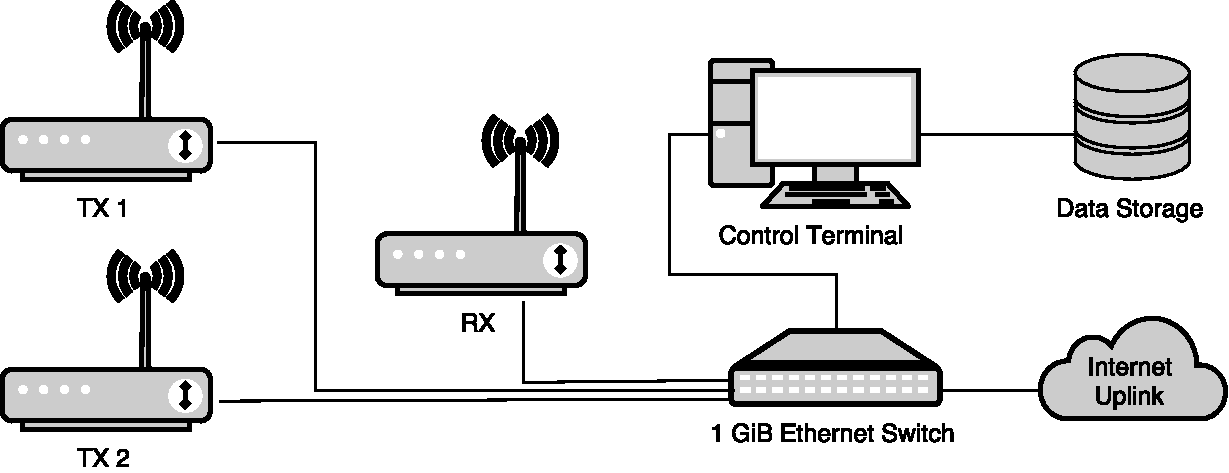
\includegraphics[width=\textwidth]{gfx/images/warp-layout}
	\caption{WARP SDR Experiments Hardware Layout}
	\label{fig:warp-layout}
\end{figure}

The experiments were carried out in a typical office building. This means that there were multiple IEEE 802.11 networks with several dozens of connected clients. I used a standard WLAN channel and no electromagnetic shielding.\\

Since the \gls{WARP} boards use a sampling frequency of 40 MHz, but the Matlab WLAN Systems Toolbox creates time-domain samples with a 20 MHz sampling rate, I used interpolation to adapt frequencies. This is done with the built-in \texttt{resample} Matlab function. Listing \ref{lst:resample} illustrates the process.

\begin{lstlisting}[captionpos=b,caption={Interpolate Sampling Rate},label=lst:resample]
% Interpolate to get from 20 to 40 MHz sampling rate
tx1 = resample(tx1, 40, 20);
\end{lstlisting}

For the real-world experiments, I deliberately caused frame collisions with the same scrambler initialization and destination \gls{MAC} addresses, and used \gls{MCS} 0. This means that in principal everything was the same as for the most basic simulation experiments.

To assess the basic mechanics of receiving collisions with the \glspl{SDR}, I applied cross-correlation to only one \gls{LTF} symbol instead of the \gls{MAC} addresses and plotted the results. They can be seen in figure \ref{fig:warp_preamble_corr}. The collided frames were aligned with some offset for this experiment.

While one group of spikes is a bit lower than the other, it is still easily possible to detect that there is a collision due to the 4 higher and 2 lower spikes caused by the two \glspl{LTF}. The higher level of noise in the begining of the signal are caused by \gls{AGC} in the receiving \gls{SDR}. Since the \gls{MAC} addresses are located further into the signal, and only that part is correlated for sender detection, this noise should be no problem.

\begin{figure}[H]
	\centering
  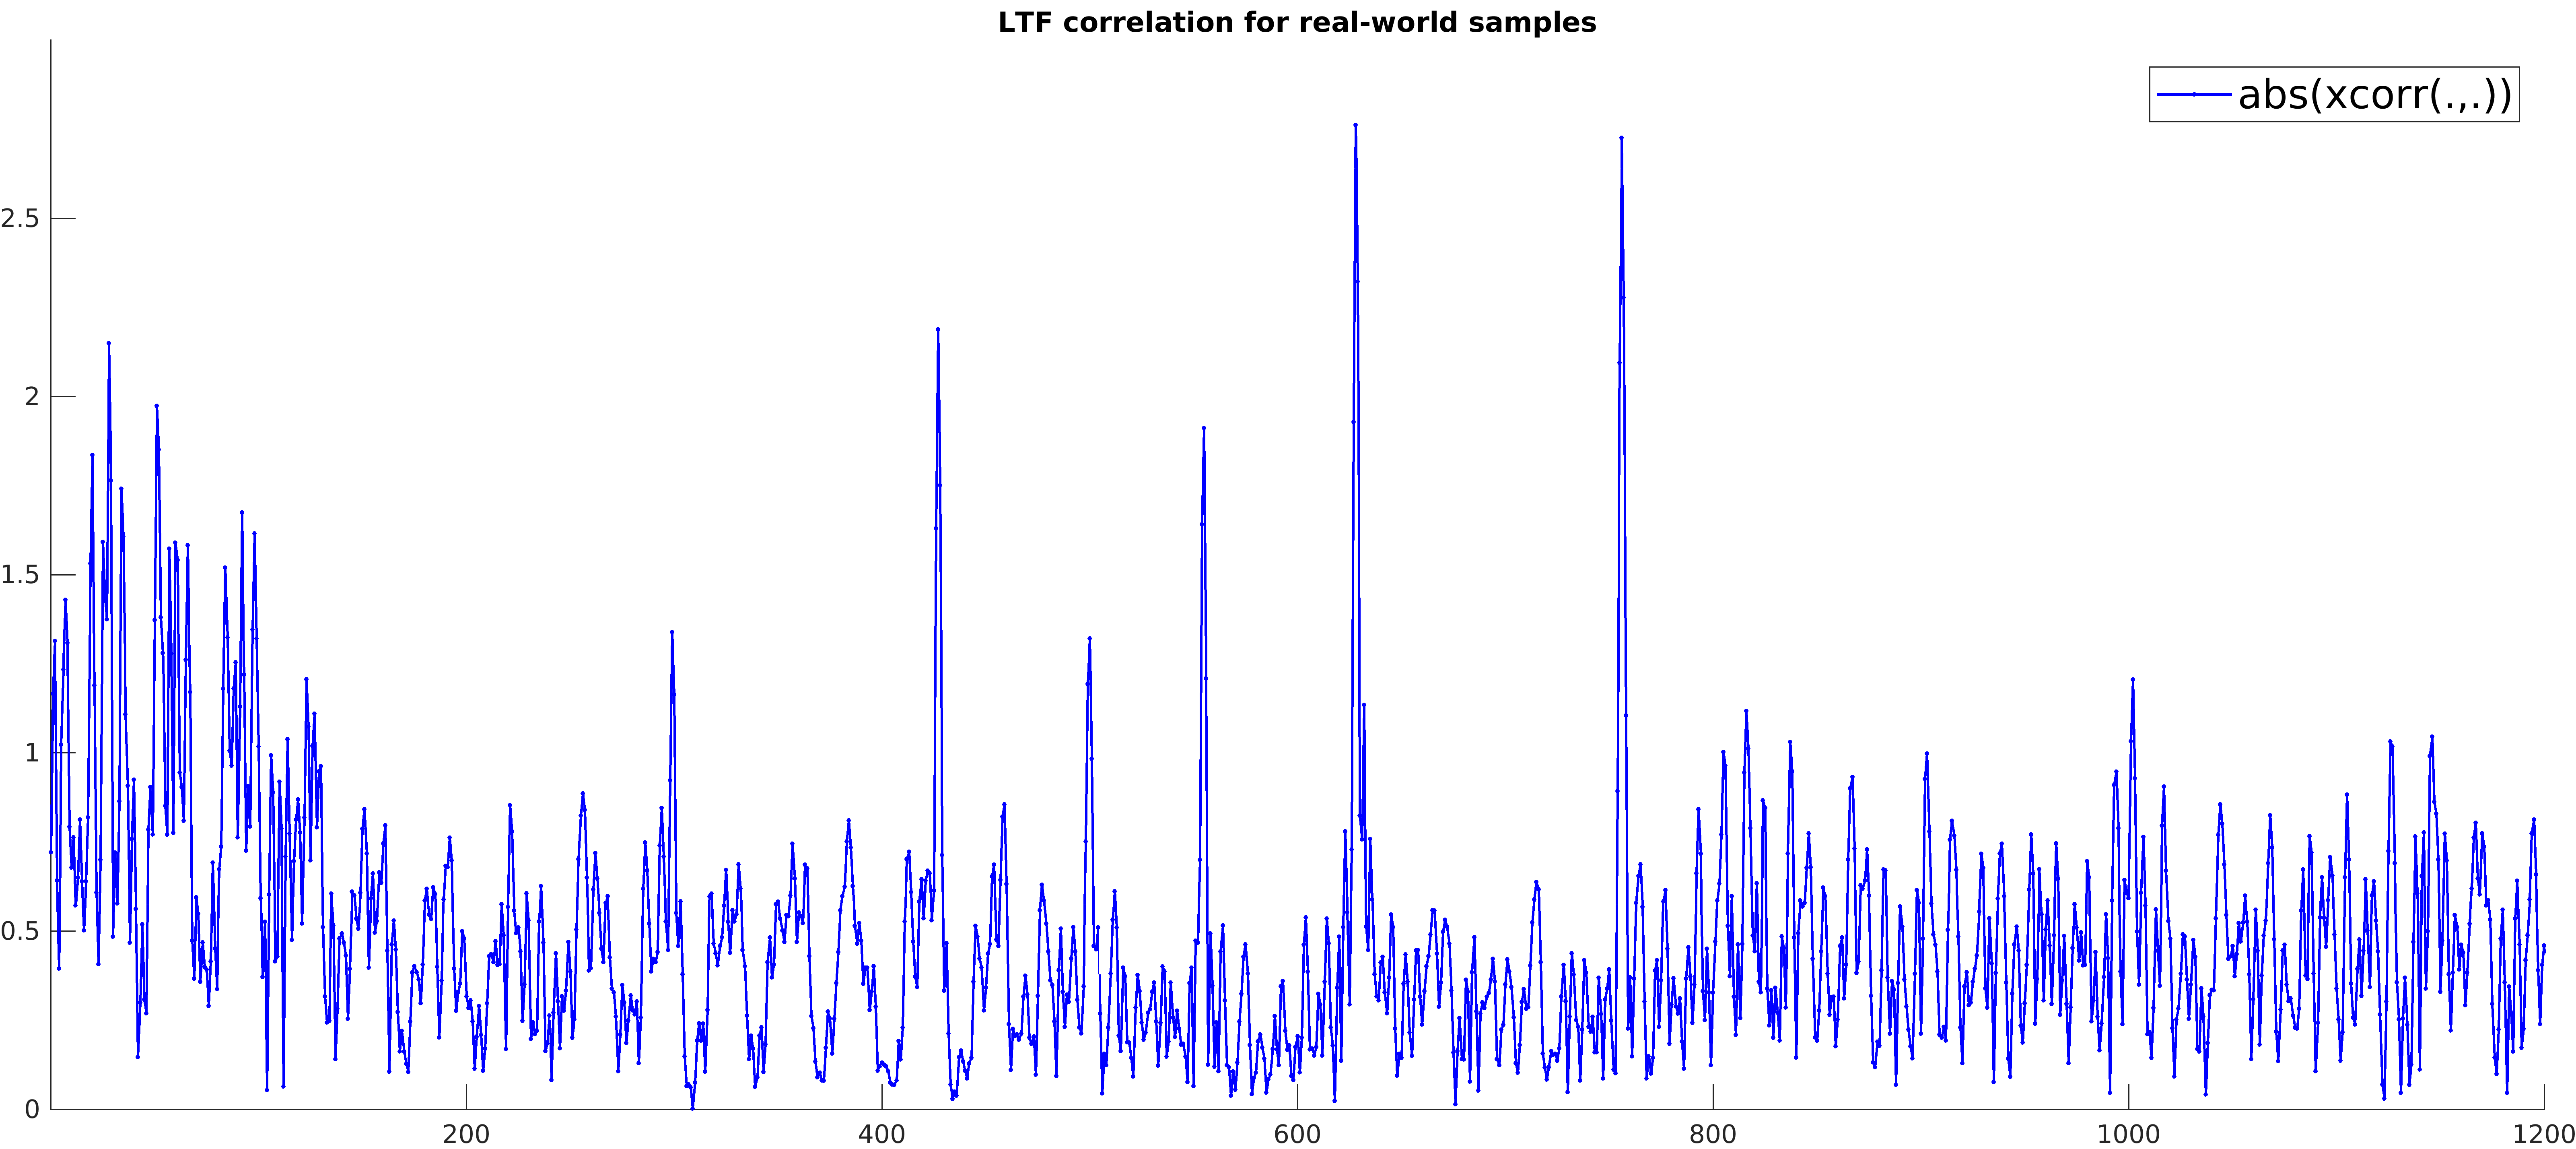
\includegraphics[width=\textwidth]{gfx/plots/capture_collision-20170622-1533-ltf_correlation}
	\caption{Preamble Correlation in WARP Experiment}
	\label{fig:warp_preamble_corr}
\end{figure}

The results of the preamble correlation are promising. They show that indeed a collision of two frames is captured by the receiving \gls{SDR}, and that cross-correlation in the time-domain can in fact tell apart both \glspl{LTF}.

Next, I used the same code as for the simulation experiments to try and detect sender \gls{MAC} addresses. Fortunately, this worked well. In general, the results were very comparable to those of the simulation, however there was a slightly lower accuracy. The reason for that is probably the channel effects, which could not be simulated in full detail by the channel models.

%% -----------------------------------------------------------------------------

\chapter{Discussion}\label{ch:Discussion}
\glsresetall % Resets all acronyms to not used

This chapter discusses the results of the evaluation, and their implications. Finally, future work is proposed to iterate on the findings.


%% -----------------------------------------------------------------------------

\section{Computational Complexity}\label{sec:complexity}

In order to use the proposed sender detection algorithm, it must be feasible to do all necessary calculations in real-time. In this section, I present an analysis of the computational complexity of the different components.

Two main categories of tasks can be identified. First, the generation of reference signals to use for cross-correlation. This can be pre-computed before any collisions are received and is therefore less time-critical. Second, correlating time-domain samples with the reference signals and sorting to work out a guess which senders participated. This needs to be done for every analyzed collision.\\

Based on the results from the experiments with scrambler initialization and the destination \gls{MAC} address as described in sections \ref{sec:ex-scrambler} and \ref{sec:ex-destination}, the following factors scale up the amount of necessary reference signals:

\begin{itemize}
  \item \gls{MAC} addresses on the network
  \item \glspl{MCS}
  \item Scrambler initialization values
\end{itemize}

The destination \gls{MAC} address can be ignored. This means that the algorithm scales according to the following equation:

$$ N_{\text{RS}} = N_{\text{MAC}} \cdot N_{\text{MCS}} \cdot N_{\text{SI}} = N_{\text{MAC}} \cdot 8 \cdot 127 $$\vspace{0cm}

Here, $ N_{\text{RS}} $ denotes the number of modulated reference signals, $ N_{\text{MCS}} $ is the number of available \glspl{MCS}, and $ N_{\text{SI}} $ describes the amount of possible scrambler initialization values.

Let $ n = N_{\text{MAC}} $ be the number of cached \gls{MAC} addresses on the network. The worst-case asymmetric complexity in this case is:

$$ O(\text{"Sender ~Detection"}) = O(n \cdot 8 \cdot 127) = O(1016 n) = O(n) $$\vspace{0cm}

The algorithm scales linearly with the amount of stations on the IEEE 802.11 network. This is optimal since every station is a possible sender which has to be considered when decoding a collision. It is however debatable whether the linear factor of 1016 is feasible on commodity computing hardware. That would be necessary to enable broad usage of the detection technique across many different devices as mentioned in chapter \ref{ch:introduction}. A quantitative analysis is therefore desirable.\\

I used the Matlab profiler to gather data on the execution speeds of different parts of the algorithm. These measurements were done on a consumer laptop, featuring a 2-core 3rd-generation Intel i3 processor with Hyper-Threading at 1.9 GHz. The results are summarized in table \ref{tbl:timing}.

\begin{table}[ht]
	\centering
	\begin{tabular}{|p{8.5cm}|p{2.5cm}|}
		\hline
		\textbf{Function} & \textbf{Time Spent} \\ \hline
	    wlanTGnChannel & 912 ms \\ \hline
    	wlanNonHTData & 662 ms \\ \hline
	    CRC Calculation & 122 ms \\ \hline
	    awgn & 54 ms \\ \hline
		xcorr & < 1 ms \\ \hline
	\end{tabular}
	\caption{Timing Analysis of the Detecting Algorithm \label{tbl:timing}}
\end{table}

This data suggests that the real-time part of the algorithm, which is limited to cross-correlation with \texttt{xcorr} is negligible when compared to the pre-modulation of reference signals. For small networks, the correlation time is probably fast enough. For high amount of stations however, the complexity gets out of hand quite quickly. For a network with 500 client for example, each collision requires a calculation of about 500 seconds due to the linear scaling factor of 1016. However, it is easily possible to parallelize this workload, or even use specialized hardware such as \glspl{FPGA}. In the extreme case, where every correlation is done at the same time, only 1 ms is needed for decoding the collision.

The calculation of \gls{CRC} checksums is time-consuming, however not needed for the algorithm. Instead, dummy checksums can be used as described in section \ref{sec:matlab-impl}. Therefore, modulation of reference signals scales with the performance of the \texttt{wlanNonHTData} function.

Since the modulation of reference signals can be done ahead of time, the only important case is that of a newly connected client. In this case, 1016 new signals must be created for this new \gls{MAC} address, which takes about 5 minutes without any parallelization. With more CPU cores however, this seems manageable.


%% -----------------------------------------------------------------------------

\section{Detection Quality}\label{sec:detection-quality}

The results of my simulations were very promising. While admittedly only IEEE 802.11 a/g networks were evaluated, as section \ref{sec:mimo} discusses further, detection accuracy was quite high even for higher \glspl{MCS}.\\

In contrast to the scrambler initialization, the value of the preceding destination \gls{MAC} address had hardly any effect on detection quality, as described in section \ref{sec:ex-destination}. Most likely this is because of the relatively small state of the convolutional encoder compared to the size of a \gls{MAC} address. While the encoder considers the last seen seven bits for its output, a \gls{MAC} address comprises 48 bits of data.

Regardless of the preceding destination \gls{MAC} address, the convolutional encoder state is synchronized after the first seven bits of the sender address. This is only a small fraction of about 15 \%. In addition to that, the first seven bits are part of the vendor prefix, which is already to some extent likely to be the same across multiple stations on the network. Therefore, convolutional encoding poses no critical impact on sender detection performance.\\

Using real-world \glspl{SDR}, the detection technique performed reasonably well at least for lower \glspl{MCS}. This is particularly nice because these experiments were conducted in an environment where production wireless traffic was present. Although there was some decrease in detection quality, this shows that the algorithm is capable of successfully recognizing sender \gls{MAC} addresses even when a reasonably high network load is present.


%% -----------------------------------------------------------------------------

\section{IEEE 802.11 n/ac/ax Networks}\label{sec:mimo}

This thesis only covered sender detection for IEEE 802.11 a/g networks. However, such networks are rarely used nowadays due to their low throughput. Modern standards such as IEEE 802.11 n/ac, and the upcoming 802.11 ax are much more relevant.

There are many improvements and differences introduced with the 802.11 n standard. One of the most important with respect to time-domain sample cross-correlation is the adoption of \gls{MIMO} transmission. With this technique, every sender and receiver uses multiple antennas, instead of just one as with 802.11 a/g. This allows for a much higher spectral efficiency, meaning that more bits can be transmitted per used bandwidth \cite{perahia2013}. However, the overall system complexity and multi-path effects in particular make it much more difficult to apply naive time-domain correlation.\\

It would be interesting whether the proposed sender detection algorithm can be adapted to work in a \gls{MIMO} environment. In the current form, this is unfortunately quite unlikely. On the one hand, collision detection and especially the determination of relevant sample periods containing the sender \gls{MAC} addresses must be adjusted to the physical layer high-throughput frame format used by modern standards \cite{ieee2012}.

On the other hand, using multiple streams implies the possibility that the sender \gls{MAC} address gets fragmented. While some bits could be transmitted in the first stream, the remaining bits could be sent in various other streams. This renders simple cross-correlation with \texttt{xcorr} directly on the received sample vector useless.


%% -----------------------------------------------------------------------------

\section{Future Work}

The preceding discussion reveals some serious problems with the proposed algorithm for sender \gls{MAC} address detection. The fundamental principles however do seem promising. There are remaining questions that should be addressed in further research.\\

\textit{Quantitative Noise Evaluation with SDRs}\\

As mentioned in section \ref{sec:detection-quality}, noise from other stations in the network could cause the correlation of \gls{MAC} addresses to degrade. Whether this is the case, and to which extent it influences detection performance, could be evaluated in a quantitative analysis. As a first step, the experiments with \gls{WARP} \glspl{SDR} should be reproduced in a radiation-free environment, such as a Faraday cage. If the technique performs better in that case, additional IEEE 802.11 devices could be added one at a time, continuously measuring the algorithm's accuracy.\\

\textit{MIMO and IEEE 802.11 n/ac/ax}\\

In a next step, the technique could be adapted to current IEEE 802.11 standards, such as 802.11 n/ac. This involves finding a solution to the problems with \gls{MIMO}, as described in section \ref{sec:mimo}, especially the fragmentation of \gls{MAC} address bits onto different spatial transmission streams.\\

\textit{Implementation on Mobile Operating Systems}\\

In order to be used with possible new \glspl{DCF}, it is interesting how the sender detection algorithm performs on mobile operating systems, Android and Apple iOS in particular. Since almost everybody has a smartphone these days, those operating systems power a significant fraction of stations in IEEE 802.11 networks. While desktop operating systems are also very important, mobile platforms face the additional issue that due to limited battery power, calculations are inherently more expensive.

Future work could implement sender detection on collisions as a kernel module for mobile platforms and evaluate its performance and accuracy. A special focus should be set to complexity, power usage, and overall implications on device usability and responsiveness.

%% -----------------------------------------------------------------------------

\chapter{Conclusion}\label{ch:Conclusion}
\glsresetall % Resets all acronyms to not used

Recognizing senders by correlating their \gls{MAC} addresses in an IEEE 802.11 a/g frame collision is an approach that to my knowledge has not been explored before. In this thesis, I proposed an algorithm to apply this technique and developed a proof-of-concept implementation using Matlab with the Communications and WLAN Systems Toolboxes.\\

The technique promiscuously listens on the wireless network interface to cache \gls{MAC} addresses of stations connected to the network. For each of these addresses, several reference signals are pre-modulated and stored, considering different \glspl{MCS} and scrambler initialization values. When a collision is received, samples containing the \gls{MAC} address are cross-correlated in the time-domain. The reference signals with highest correlations are used to determine the senders participating in the collided transmission.\\

I evaluated the performance and accuracy of this algorithm using simulations. Even for higher \glspl{MCS}, the technique performed very well. Varying the scrambler initialization caused severe regression, whereas the destination \gls{MAC} address, preceding the sender, played a minor role. Simulations with standard channel models showed measurable impact, however up to a certain point sender detection retained a reasonable accuracy.\\

Experiments with real hardware, on three \gls{WARP} \glspl{SDR} in particular, showed promising results. Receiving a collision, correlating the frame preambles, and measuring a delay between two collided frames worked very well. Detecting sender \gls{MAC} addresses was similar to simulations and provided reasonable sender guesses. Due to channel effects, the accuracy was however reduced.\\

The proposed algorithm is not directly applicable to current versions of the IEEE 802.11 standard using \gls{MIMO}. This is due to possible spatial fractioning of the time-domain samples containing the sender \gls{MAC} address, rendering naive cross-correlation useless.\\

Future work could quantize channel effects on real hardware, and adapt the detection technique to modern IEEE 802.11 n/ac/ax standards and \gls{MIMO} transmissions.

In summary, sender detection by using cross-correlation in the time-domain worked surprisingly well despite some problems and should be explored in more detail.



%% -----------------------------------------------------------------------------

\cleardoublepage%% ---------------------------------------------------------------------------------------------------------------------
% Bibliography


% work-around to have small caps also here in the headline
\manualmark
\markboth{\spacedlowsmallcaps{\bibname}}{\spacedlowsmallcaps{\bibname}} % work-around to have small caps also
%\phantomsection 
\refstepcounter{dummy}
\addtocontents{toc}{\protect\vspace{\beforebibskip}} % to have the bib a bit from the rest in the toc
\addcontentsline{toc}{chapter}{\tocEntry{\bibname}}
\label{app:bibliography}
\printbibliography

\cleardoublepage%% ---------------------------------------------------------------------------------------------------------------------
%  Declaration


%\refstepcounter{dummy}
%\pdfbookmark[0]{Thesis Statement}{statement} \chapter*{Thesis Statement}
%\thispagestyle{empty}
%\begingroup
%\let\cleardoublepage\relax
%\begin{flushright}
%	\emph{pursuant to §\,22 paragraph 7 of APB TU Darmstadt}
%\end{flushright}
%I herewith formally declare that I have written the submitted \myDegree{} independently. I did not use any outside support except for the quoted literature and other sources mentioned in the paper. I clearly marked and separately listed all of the literature and all of the other sources which I employed when producing this academic work, either literally or in content. This thesis has not been handed in or published before in the same or similar form.
%In the submitted thesis the written copies and the electronic version are identical in content.
%
%\bigskip
%
%\noindent\textit{\myLocation, \myTime}
%
%\smallskip
%
%\begin{flushright}
%	\begin{tabular}{m{5cm}}
%		\\ \hline
%		\centering\myName \\
%	\end{tabular}
%\end{flushright}
%
%\vfill

\selectlanguage{ngerman}
\pdfbookmark[0]{Erklärung zur Abschlussarbeit}{erklaerung} \chapter*{Erklärung zur Abschlussarbeit}
\begin{flushright}
	\emph{gemäß §\,22 Abs.\,7 APB der TU Darmstadt}
\end{flushright}
Hiermit versichere ich, \myName{}, die vorliegende \myDegree{} ohne Hilfe Dritter und nur mit den angegebenen Quellen und Hilfsmitteln angefertigt zu haben. Alle Stellen, die Quellen entnommen wurden, sind als solche kenntlich gemacht worden. Diese Arbeit hat in gleicher oder ähnlicher Form noch keiner Prüfungsbehörde vorgelegen.

Mir ist bekannt, dass im Falle eines Plagiats (§38 Abs.2 APB) ein Täuschungsversuch vorliegt, der dazu führt, dass die Arbeit mit 5,0 bewertet und damit ein Prüfungsversuch verbraucht wird. Abschlussarbeiten dürfen nur einmal wiederholt werden.

Bei der abgegebenen Thesis stimmen die schriftliche und die zur Archivierung eingereichte elektronische Fassung überein.

\bigskip

\noindent\textit{\myLocation, \myTime}

\smallskip

\begin{flushright}
    \begin{tabular}{m{5cm}}
        \\ \hline
        \centering\myName \\
    \end{tabular}
\end{flushright}

\selectlanguage{american}



\end{document}
